\documentclass[10pt]{article}\usepackage[]{graphicx}\usepackage[]{color}
%% maxwidth is the original width if it is less than linewidth
%% otherwise use linewidth (to make sure the graphics do not exceed the margin)
\makeatletter
\def\maxwidth{ %
  \ifdim\Gin@nat@width>\linewidth
    \linewidth
  \else
    \Gin@nat@width
  \fi
}
\makeatother

\definecolor{fgcolor}{rgb}{0.345, 0.345, 0.345}
\newcommand{\hlnum}[1]{\textcolor[rgb]{0.686,0.059,0.569}{#1}}%
\newcommand{\hlstr}[1]{\textcolor[rgb]{0.192,0.494,0.8}{#1}}%
\newcommand{\hlcom}[1]{\textcolor[rgb]{0.678,0.584,0.686}{\textit{#1}}}%
\newcommand{\hlopt}[1]{\textcolor[rgb]{0,0,0}{#1}}%
\newcommand{\hlstd}[1]{\textcolor[rgb]{0.345,0.345,0.345}{#1}}%
\newcommand{\hlkwa}[1]{\textcolor[rgb]{0.161,0.373,0.58}{\textbf{#1}}}%
\newcommand{\hlkwb}[1]{\textcolor[rgb]{0.69,0.353,0.396}{#1}}%
\newcommand{\hlkwc}[1]{\textcolor[rgb]{0.333,0.667,0.333}{#1}}%
\newcommand{\hlkwd}[1]{\textcolor[rgb]{0.737,0.353,0.396}{\textbf{#1}}}%
\let\hlipl\hlkwb

\usepackage{framed}
\makeatletter
\newenvironment{kframe}{%
 \def\at@end@of@kframe{}%
 \ifinner\ifhmode%
  \def\at@end@of@kframe{\end{minipage}}%
  \begin{minipage}{\columnwidth}%
 \fi\fi%
 \def\FrameCommand##1{\hskip\@totalleftmargin \hskip-\fboxsep
 \colorbox{shadecolor}{##1}\hskip-\fboxsep
     % There is no \\@totalrightmargin, so:
     \hskip-\linewidth \hskip-\@totalleftmargin \hskip\columnwidth}%
 \MakeFramed {\advance\hsize-\width
   \@totalleftmargin\z@ \linewidth\hsize
   \@setminipage}}%
 {\par\unskip\endMakeFramed%
 \at@end@of@kframe}
\makeatother

\definecolor{shadecolor}{rgb}{.97, .97, .97}
\definecolor{messagecolor}{rgb}{0, 0, 0}
\definecolor{warningcolor}{rgb}{1, 0, 1}
\definecolor{errorcolor}{rgb}{1, 0, 0}
\newenvironment{knitrout}{}{} % an empty environment to be redefined in TeX

\usepackage{alltt}
\usepackage{amsfonts,amssymb,amsbsy,amsmath,latexsym,natbib,graphicx}
\usepackage{subfigure,color}
\usepackage{fullpage}
\IfFileExists{upquote.sty}{\usepackage{upquote}}{}
\begin{document}

\title{National University of Singapore\\
\bigskip\\
ST3233: Applied Time Series Analysis\\
Assignment 2\\
\bigskip
\small{Final Version}\\
}
\bigskip
\author{Ye Rong}
\bigskip
\date{Oct.29.2016}
\maketitle


\tableofcontents

\newpage

\section{ Exercise 1 (Can one trust confidence intervals?)}

\begin{knitrout}
\definecolor{shadecolor}{rgb}{0.969, 0.969, 0.969}\color{fgcolor}\begin{kframe}
\begin{alltt}
\hlkwd{library}\hlstd{(forecast)}
\hlkwd{library}\hlstd{(fpp)}
\end{alltt}


{\ttfamily\noindent\itshape\color{messagecolor}{\#\# Loading required package: fma}}

{\ttfamily\noindent\itshape\color{messagecolor}{\#\# Loading required package: expsmooth}}

{\ttfamily\noindent\itshape\color{messagecolor}{\#\# Loading required package: lmtest}}

{\ttfamily\noindent\itshape\color{messagecolor}{\#\# Loading required package: zoo}}

{\ttfamily\noindent\itshape\color{messagecolor}{\#\# \\\#\# Attaching package: 'zoo'}}

{\ttfamily\noindent\itshape\color{messagecolor}{\#\# The following objects are masked from 'package:base':\\\#\# \\\#\#\ \ \ \  as.Date, as.Date.numeric}}

{\ttfamily\noindent\itshape\color{messagecolor}{\#\# Loading required package: tseries}}\end{kframe}
\end{knitrout}
1. Fit a SARIMA model

\begin{knitrout}
\definecolor{shadecolor}{rgb}{0.969, 0.969, 0.969}\color{fgcolor}\begin{kframe}
\begin{alltt}
\hlkwd{load}\hlstd{(}\hlstr{"E:/ST3233/Assignment2/Datasets/tsa3.rda"}\hlstd{)}
\hlkwd{plot}\hlstd{(birth,}\hlkwc{lwd} \hlstd{=} \hlnum{2} \hlstd{,}\hlkwc{main} \hlstd{=} \hlstr{"Monthly Birth(in thousand)"}\hlstd{)}
\end{alltt}
\end{kframe}
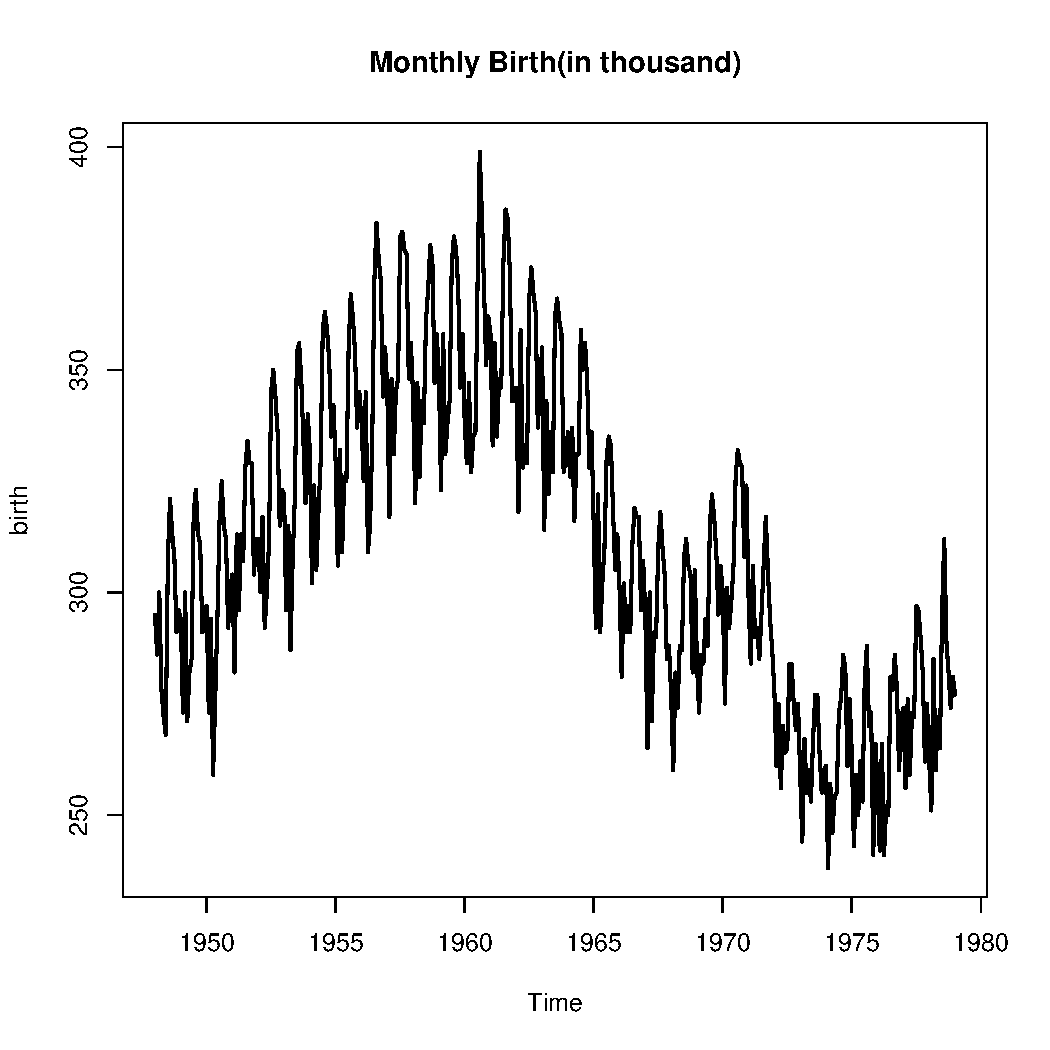
\includegraphics[width=\maxwidth]{figure/unnamed-chunk-2-1} 

\end{knitrout}
From the plot, seasonal component = 12, so we differentiate it twice: lag = 12, lag = 1, and apply SARIMA model.

\begin{knitrout}
\definecolor{shadecolor}{rgb}{0.969, 0.969, 0.969}\color{fgcolor}\begin{kframe}
\begin{alltt}
\hlstd{birth_d12} \hlkwb{<-} \hlkwd{diff}\hlstd{(birth,} \hlkwc{lag} \hlstd{=} \hlnum{12}\hlstd{)}
\hlkwd{plot}\hlstd{(birth_d12,}\hlkwc{lwd} \hlstd{=} \hlnum{2}\hlstd{,}\hlkwc{main} \hlstd{=} \hlstr{"diff(birth, lag = 12)"}\hlstd{)}
\end{alltt}
\end{kframe}
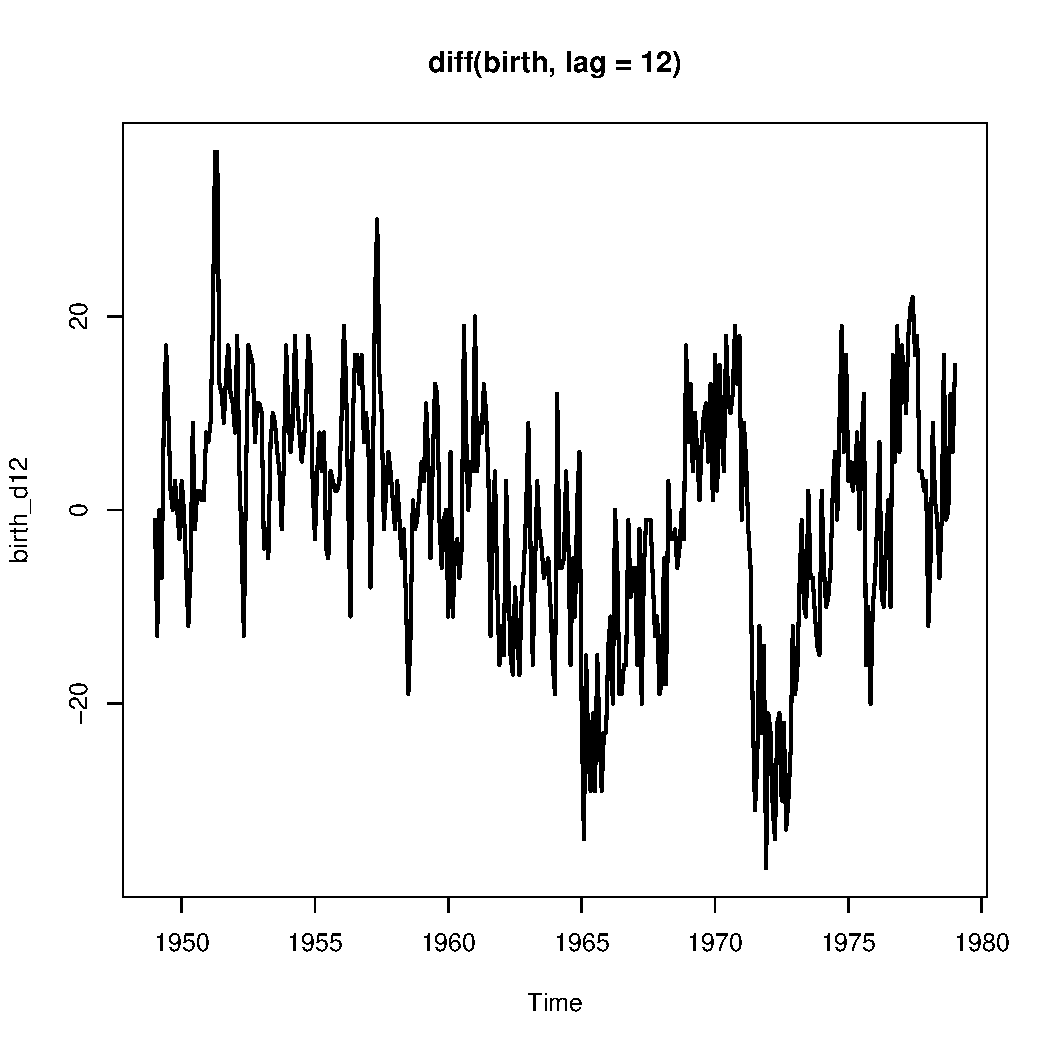
\includegraphics[width=\maxwidth]{figure/unnamed-chunk-3-1} 
\begin{kframe}\begin{alltt}
\hlstd{birth_d12_d1} \hlkwb{<-} \hlkwd{diff}\hlstd{(birth_d12,}\hlkwc{lag} \hlstd{=} \hlnum{1}\hlstd{)}
\hlkwd{plot}\hlstd{(birth_d12_d1,}\hlkwc{lwd} \hlstd{=} \hlnum{2}\hlstd{,}\hlkwc{main} \hlstd{=} \hlstr{"diff(diff(birth, lag = 12))"}\hlstd{)}
\end{alltt}
\end{kframe}
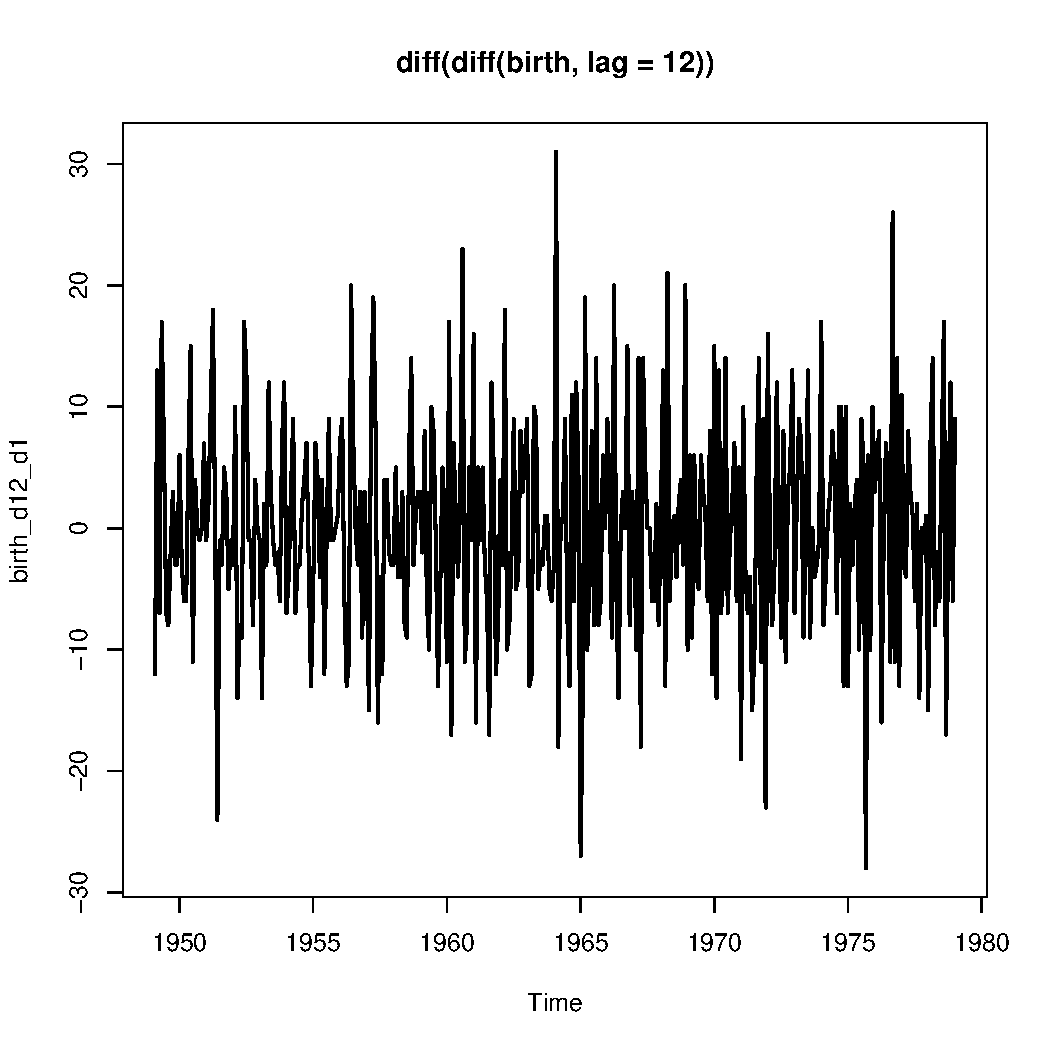
\includegraphics[width=\maxwidth]{figure/unnamed-chunk-3-2} 
\begin{kframe}\begin{alltt}
\hlkwd{par}\hlstd{(}\hlkwc{mfrow}\hlstd{=}\hlkwd{c}\hlstd{(}\hlnum{2}\hlstd{,}\hlnum{1}\hlstd{))}
\hlkwd{acf}\hlstd{(birth_d12_d1,}\hlkwc{lwd} \hlstd{=} \hlnum{3}\hlstd{,} \hlkwc{main} \hlstd{=} \hlstr{"ACF::diff(diff(birth, lag = 12))"}\hlstd{)}
\hlkwd{pacf}\hlstd{(birth_d12_d1,}\hlkwc{lwd} \hlstd{=} \hlnum{3}\hlstd{,} \hlkwc{main} \hlstd{=} \hlstr{"PACF::diff(diff(birth, lag = 12))"}\hlstd{)}
\end{alltt}
\end{kframe}
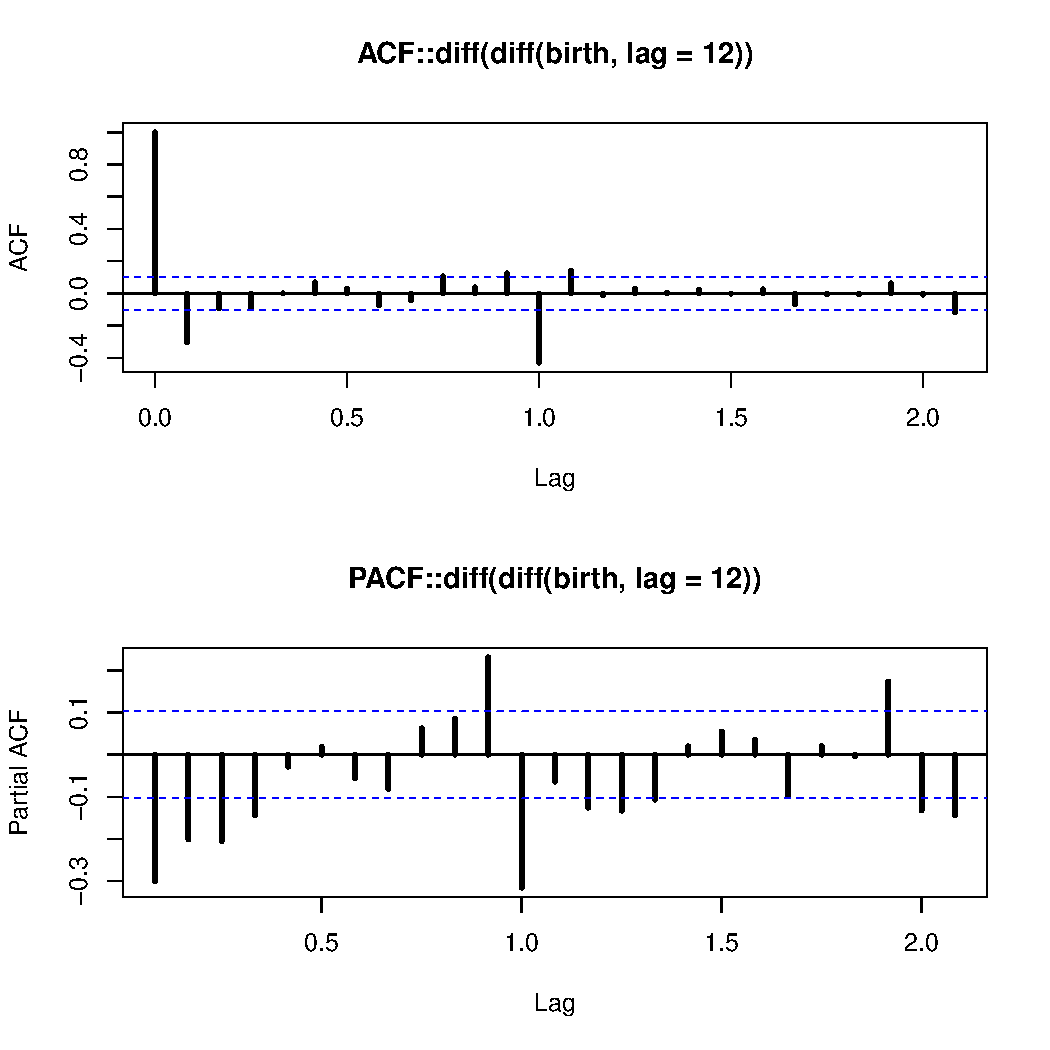
\includegraphics[width=\maxwidth]{figure/unnamed-chunk-3-3} 

\end{knitrout}
From acf plot ,q \leq 1, and from partial-acf plot, p \leq 4. 
For SARIMA model, generally, P,Q \leq 1

\begin{knitrout}
\definecolor{shadecolor}{rgb}{0.969, 0.969, 0.969}\color{fgcolor}\begin{kframe}
\begin{alltt}
\hlstd{AIC_best} \hlkwb{=} \hlnum{10}\hlopt{**}\hlnum{6}
\hlstd{k} \hlkwb{<-}  \hlnum{0}
\hlkwa{for}\hlstd{(p} \hlkwa{in} \hlnum{0}\hlopt{:}\hlnum{4}\hlstd{)\{}
  \hlkwa{for}\hlstd{(q} \hlkwa{in} \hlnum{0}\hlopt{:}\hlnum{1}\hlstd{)\{}
    \hlkwa{for}\hlstd{(P} \hlkwa{in} \hlnum{0}\hlopt{:}\hlnum{1}\hlstd{)\{}
      \hlkwa{for}\hlstd{(Q} \hlkwa{in} \hlnum{0}\hlopt{:}\hlnum{1}\hlstd{)\{}
        \hlstd{fit_sarima} \hlkwb{=} \hlkwd{Arima}\hlstd{(birth,} \hlkwc{order} \hlstd{=} \hlkwd{c}\hlstd{(p,}\hlnum{1}\hlstd{,q),} \hlkwc{seasonal} \hlstd{=} \hlkwd{c}\hlstd{(P,}\hlnum{1}\hlstd{,Q))}
        \hlkwa{if} \hlstd{(fit_sarima}\hlopt{$}\hlstd{aic} \hlopt{<} \hlstd{AIC_best)\{}
          \hlstd{k} \hlkwb{=} \hlstd{k} \hlopt{+} \hlnum{1}
          \hlstd{AIC_best} \hlkwb{<-} \hlstd{fit_sarima}\hlopt{$}\hlstd{aic}
          \hlkwd{cat}\hlstd{(}\hlstr{"model"}\hlstd{,k,}\hlstr{"\textbackslash{}t p="}\hlstd{,p,}\hlstr{"q="}\hlstd{,q,}\hlstr{"P="}\hlstd{,P,}\hlstr{"Q="}\hlstd{,Q,}\hlstr{"\textbackslash{}t AIC="}\hlstd{,}
              \hlstd{AIC_best,}\hlstr{"\textbackslash{}t Number of parameters="}\hlstd{, p}\hlopt{+}\hlstd{q}\hlopt{+}\hlstd{P}\hlopt{+}\hlstd{Q,} \hlstr{"\textbackslash{}n"}\hlstd{)}
        \hlstd{\}}
      \hlstd{\}}
    \hlstd{\}}
  \hlstd{\}}
\hlstd{\}}
\end{alltt}
\begin{verbatim}
## model 1 	 p= 0 q= 0 P= 0 Q= 0 	 AIC= 2621.434 	 Number of parameters= 0 
## model 2 	 p= 0 q= 0 P= 0 Q= 1 	 AIC= 2472.199 	 Number of parameters= 1 
## model 3 	 p= 0 q= 1 P= 0 Q= 1 	 AIC= 2428.557 	 Number of parameters= 2 
## model 4 	 p= 1 q= 1 P= 0 Q= 1 	 AIC= 2419.855 	 Number of parameters= 3 
## model 5 	 p= 1 q= 1 P= 1 Q= 1 	 AIC= 2419.66 	 Number of parameters= 4 
## model 6 	 p= 4 q= 0 P= 0 Q= 1 	 AIC= 2417.468 	 Number of parameters= 5
\end{verbatim}
\end{kframe}
\end{knitrout}
From the output, since SARIMA((4,1,0)(0,1,1)[12]) gives lowest AIC, we choose it.(number of parameters = 4+0+0+1 = 5)
\begin{knitrout}
\definecolor{shadecolor}{rgb}{0.969, 0.969, 0.969}\color{fgcolor}\begin{kframe}
\begin{alltt}
\hlstd{birth_fit} \hlkwb{<-} \hlkwd{Arima}\hlstd{(birth,} \hlkwc{order} \hlstd{=} \hlkwd{c}\hlstd{(}\hlnum{4}\hlstd{,}\hlnum{1}\hlstd{,}\hlnum{0}\hlstd{),} \hlkwc{seasonal} \hlstd{=} \hlkwd{c}\hlstd{(}\hlnum{0}\hlstd{,}\hlnum{1}\hlstd{,}\hlnum{1}\hlstd{))}
\end{alltt}
\end{kframe}
\end{knitrout}

Conclusion: The SARIMA model is : SARIMA((4,1,0)(0,1,1)[12])
\bigskip
2. Use your model to get a 80\% confidence interval for the number of births in Feb 1979.
\begin{knitrout}
\definecolor{shadecolor}{rgb}{0.969, 0.969, 0.969}\color{fgcolor}\begin{kframe}
\begin{alltt}
\hlkwd{forecast}\hlstd{(fit_sarima,} \hlkwc{h}\hlstd{=}\hlnum{1}\hlstd{)}
\end{alltt}
\begin{verbatim}
##          Point Forecast    Lo 80    Hi 80    Lo 95    Hi 95
## Feb 1979        256.856 248.1997 265.5123 243.6174 270.0946
\end{verbatim}
\end{kframe}
\end{knitrout}
Thus,the 80\% confidence interval for the number of births in Feb 1979 is [250.0562,267.3686]
\bigskip
3. Use an approach similar to cross validation to estimate whether you can trust the 80\% confidence interval.

\begin{knitrout}
\definecolor{shadecolor}{rgb}{0.969, 0.969, 0.969}\color{fgcolor}\begin{kframe}
\begin{alltt}
\hlstd{ts_length} \hlkwb{<-}  \hlkwd{length}\hlstd{(birth)}
\hlstd{forecast_length} \hlkwb{<-} \hlnum{1}
\hlstd{start} \hlkwb{<-} \hlnum{250}
\hlstd{lower_bounds} \hlkwb{<-} \hlkwd{c}\hlstd{()}
\hlstd{upper_bounds}\hlkwb{<-} \hlkwd{c}\hlstd{()}
\hlstd{correct_num} \hlkwb{<-} \hlnum{0}
\hlstd{wrong_num} \hlkwb{<-} \hlnum{0}
\hlcom{#Correct_num means the number of birth[i] in the 80% confidence interval}
\hlkwa{for}\hlstd{(i} \hlkwa{in} \hlstd{start}\hlopt{:}\hlstd{(ts_length} \hlopt{-} \hlstd{forecast_length))\{}

  \hlstd{fitted_sarima}\hlkwb{<-}  \hlkwd{Arima}\hlstd{(birth[}\hlnum{0}\hlopt{:}\hlstd{i],} \hlkwc{order} \hlstd{=} \hlkwd{c}\hlstd{(}\hlnum{4}\hlstd{,}\hlnum{1}\hlstd{,}\hlnum{0}\hlstd{),} \hlkwc{seasonal} \hlstd{=} \hlkwd{c}\hlstd{(}\hlnum{0}\hlstd{,}\hlnum{1}\hlstd{,}\hlnum{1}\hlstd{))}
  \hlstd{forecast_result} \hlkwb{<-}  \hlkwd{forecast}\hlstd{(fitted_sarima,} \hlkwc{h} \hlstd{= forecast_length)}
  \hlstd{lower_bounds[i]} \hlkwb{<-} \hlstd{forecast_result}\hlopt{$}\hlstd{lower[}\hlnum{1}\hlstd{]}
  \hlstd{upper_bounds[i]} \hlkwb{<-} \hlstd{forecast_result}\hlopt{$}\hlstd{upper[}\hlnum{1}\hlstd{]}
  \hlkwa{if} \hlstd{(birth[i}\hlopt{+}\hlnum{1}\hlstd{]} \hlopt{>} \hlstd{lower_bounds[i]} \hlopt{&} \hlstd{birth[i}\hlopt{+}\hlnum{1}\hlstd{]} \hlopt{<} \hlstd{upper_bounds[i])\{}
    \hlstd{correct_num} \hlkwb{=} \hlstd{correct_num} \hlopt{+} \hlnum{1}
  \hlstd{\}}\hlkwa{else}\hlstd{\{}
    \hlstd{wrong_num}\hlkwb{=} \hlstd{wrong_num} \hlopt{+} \hlnum{1}
  \hlstd{\}}
\hlstd{\}}

\hlstd{correct_num}
\end{alltt}
\begin{verbatim}
## [1] 104
\end{verbatim}
\begin{alltt}
\hlstd{wrong_num}
\end{alltt}
\begin{verbatim}
## [1] 19
\end{verbatim}
\begin{alltt}
\hlcom{#plot the bounds of confidence interval and the time series.}
\hlstd{upper_bounds_ts}\hlkwb{<-}\hlkwd{ts}\hlstd{(upper_bounds,} \hlkwc{start} \hlstd{=} \hlkwd{c}\hlstd{(}\hlnum{1948}\hlstd{,}\hlnum{2}\hlstd{),} \hlkwc{frequency} \hlstd{=} \hlnum{12}\hlstd{)}
\hlstd{lower_bounds_ts}\hlkwb{<-}\hlkwd{ts}\hlstd{(lower_bounds,} \hlkwc{start} \hlstd{=} \hlkwd{c}\hlstd{(}\hlnum{1948}\hlstd{,}\hlnum{2}\hlstd{),} \hlkwc{frequency} \hlstd{=} \hlnum{12}\hlstd{)}

\hlkwd{par}\hlstd{(}\hlkwc{mfrow}\hlstd{=}\hlkwd{c}\hlstd{(}\hlnum{1}\hlstd{,}\hlnum{1}\hlstd{))}
\hlkwd{plot}\hlstd{(birth,} \hlkwc{lwd} \hlstd{=}\hlnum{2}\hlstd{,} \hlkwc{main}\hlstd{=}\hlstr{"Prediction of Birth Time Series"}\hlstd{)}
\hlkwd{lines}\hlstd{(upper_bounds_ts,} \hlkwc{lwd} \hlstd{=} \hlnum{3}\hlstd{,} \hlkwc{col} \hlstd{=} \hlstr{"blueviolet"}\hlstd{)}
\hlkwd{lines}\hlstd{(lower_bounds_ts,} \hlkwc{lwd} \hlstd{=} \hlnum{3}\hlstd{,} \hlkwc{col} \hlstd{=} \hlstr{"blueviolet"}\hlstd{)}
\end{alltt}
\end{kframe}
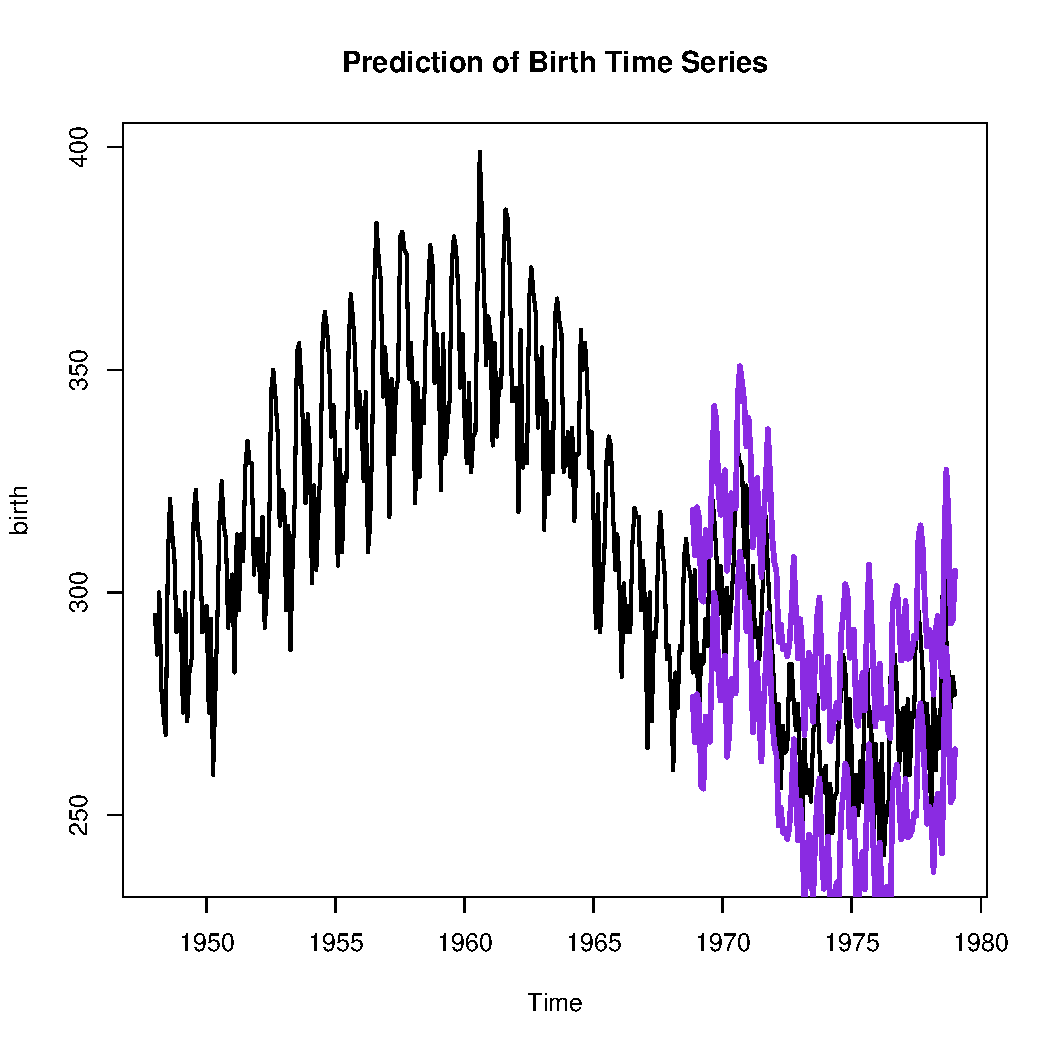
\includegraphics[width=\maxwidth]{figure/unnamed-chunk-7-1} 

\end{knitrout}
We did 123 forecasts to examine whether the true value lies in the 80\% confidence interval of prediction,
There are 104/123 in the confidence interval, and 19/123 of the forecasts doesn't.
Also, from the plot, we can trust 80\% confidence interval.


\section{ Exercise 2 (Number of Birth in California?)}

1. Load the data and plot.
\begin{knitrout}
\definecolor{shadecolor}{rgb}{0.969, 0.969, 0.969}\color{fgcolor}\begin{kframe}
\begin{alltt}
\hlstd{birth_data} \hlkwb{<-} \hlkwd{read.csv}\hlstd{(}\hlstr{"E:/ST3233/Assignment2/Datasets/daily-total-female-births-in-cal.csv"}\hlstd{,}
                       \hlkwc{header}\hlstd{=} \hlnum{TRUE}\hlstd{,}\hlkwc{sep}\hlstd{=}\hlstr{","}\hlstd{)}
\hlstd{birth_cal} \hlkwb{<-} \hlkwd{ts}\hlstd{(birth_data}\hlopt{$}\hlstd{Daily.total.female.births.in.California,}
                \hlkwc{frequency} \hlstd{=} \hlnum{356}\hlstd{,}\hlkwc{start} \hlstd{=} \hlkwd{c}\hlstd{(}\hlnum{1959}\hlstd{))}
\hlkwd{par}\hlstd{(}\hlkwc{mfrow}\hlstd{=}\hlkwd{c}\hlstd{(}\hlnum{1}\hlstd{,}\hlnum{1}\hlstd{))}
\hlkwd{plot}\hlstd{(birth_cal,}\hlkwc{lwd} \hlstd{=} \hlnum{2}\hlstd{,} \hlkwc{main} \hlstd{=} \hlstr{"Daily total female births in California"}\hlstd{)}
\end{alltt}
\end{kframe}
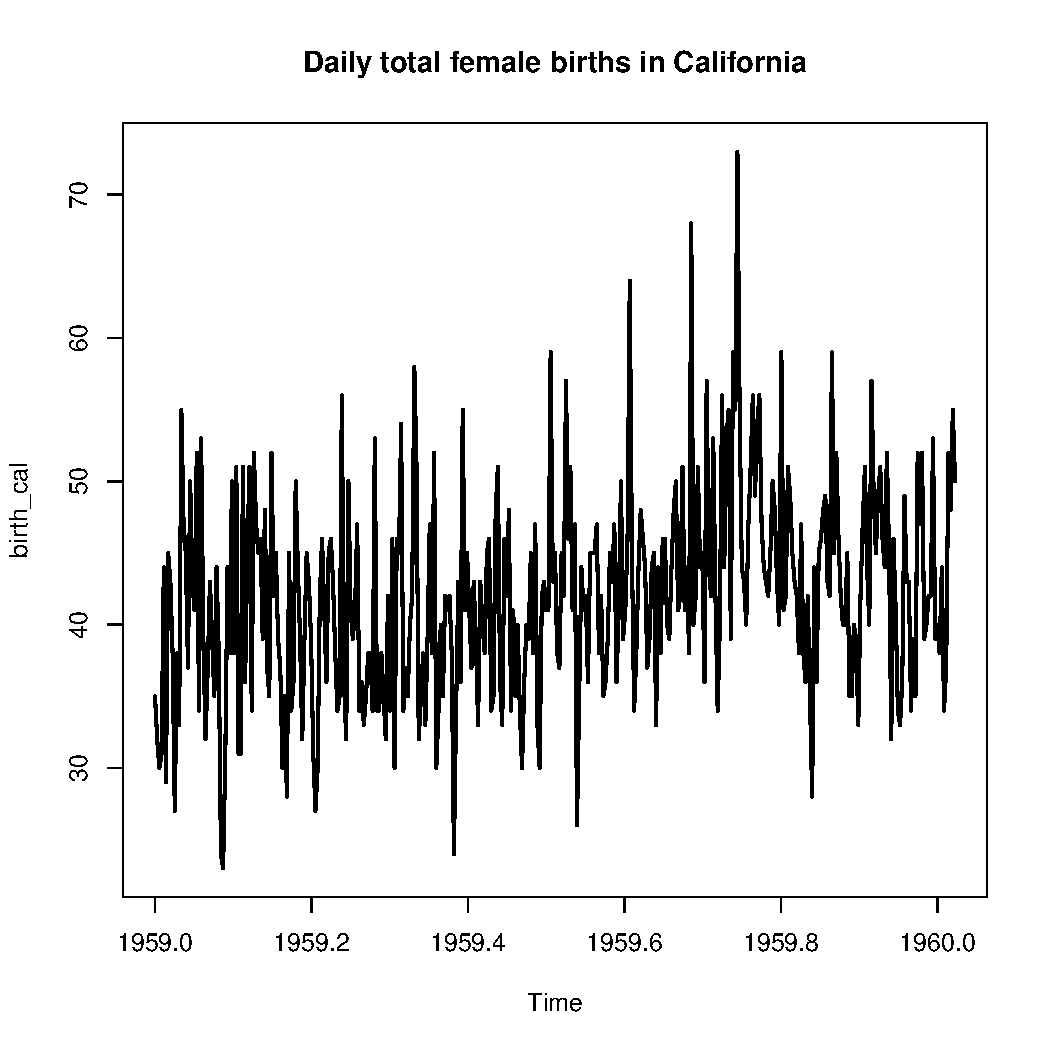
\includegraphics[width=\maxwidth]{figure/unnamed-chunk-8-1} 
\begin{kframe}\begin{alltt}
\hlcom{#Plot ACF to see whether the time series is stationary or not.}
\hlkwd{acf}\hlstd{(birth_cal,}\hlkwc{lwd} \hlstd{=} \hlnum{2}\hlstd{,} \hlkwc{main} \hlstd{=}\hlstr{"ACF::Birth in California"}\hlstd{,}\hlkwc{lag.max} \hlstd{=} \hlnum{20}\hlstd{)}
\end{alltt}
\end{kframe}
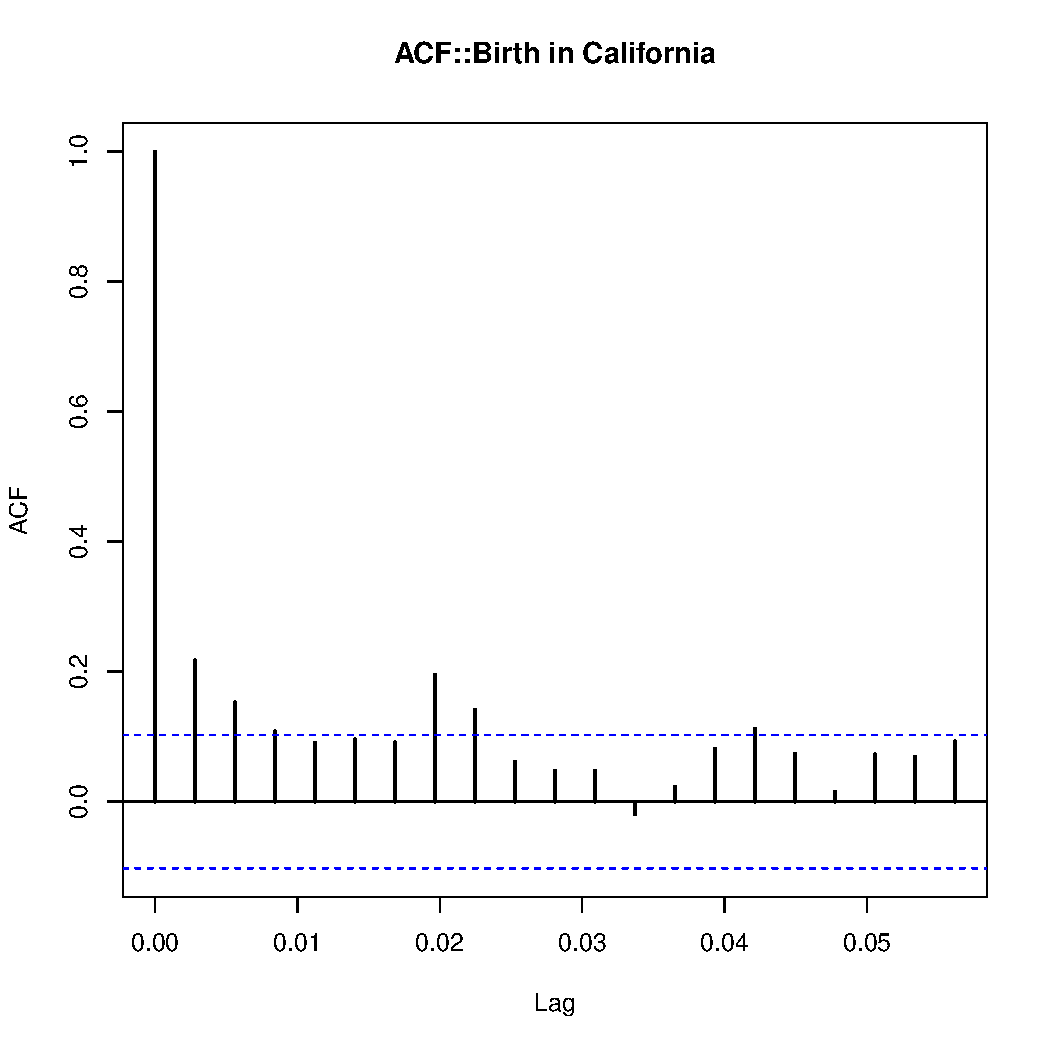
\includegraphics[width=\maxwidth]{figure/unnamed-chunk-8-2} 

\end{knitrout}
From the plot, the time series is not stationary, thus we cannot use ARMA model. Besides, there is no seasonal component in this time series, so we first choose ARIMA model.
\bigskip
2. Fit an ARIMA model.
\begin{knitrout}
\definecolor{shadecolor}{rgb}{0.969, 0.969, 0.969}\color{fgcolor}\begin{kframe}
\begin{alltt}
\hlcom{#Consider a new time series: diff(birth_cal)}
\hlstd{birth_d1} \hlkwb{=} \hlkwd{diff}\hlstd{(birth_cal)}
\hlkwd{plot}\hlstd{(birth_d1,}\hlkwc{lwd} \hlstd{=} \hlnum{2}\hlstd{,} \hlkwc{main} \hlstd{=} \hlstr{"Diff(birth in California)"}\hlstd{)}
\end{alltt}
\end{kframe}
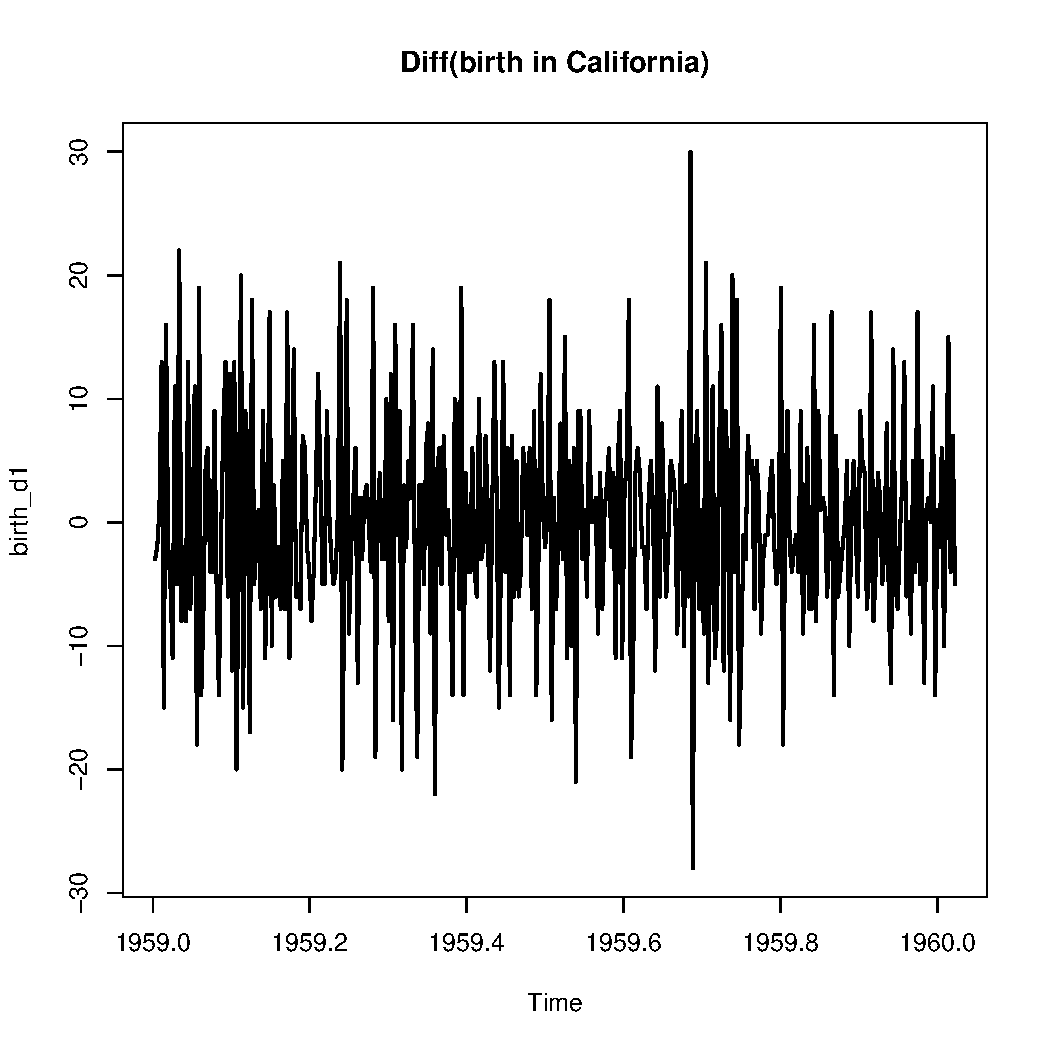
\includegraphics[width=\maxwidth]{figure/unnamed-chunk-9-1} 
\begin{kframe}\begin{alltt}
\hlcom{#Diff(birth_cal) is stationary, and then consider the acf and pacf.}

\hlkwd{par}\hlstd{(}\hlkwc{mfrow}\hlstd{=}\hlkwd{c}\hlstd{(}\hlnum{2}\hlstd{,}\hlnum{1}\hlstd{))}
\hlkwd{acf}\hlstd{(birth_d1,}\hlkwc{lwd} \hlstd{=} \hlnum{2}\hlstd{,} \hlkwc{main} \hlstd{=}  \hlstr{"ACF::diff(birth)"}\hlstd{,}\hlkwc{lag.max} \hlstd{=} \hlnum{20}\hlstd{)}
\hlkwd{pacf}\hlstd{(birth_d1,}\hlkwc{lwd} \hlstd{=} \hlnum{2}\hlstd{,} \hlkwc{main} \hlstd{=}  \hlstr{"PACF::diff(birth)"}\hlstd{,}\hlkwc{lag.max} \hlstd{=} \hlnum{20}\hlstd{)}
\end{alltt}
\end{kframe}
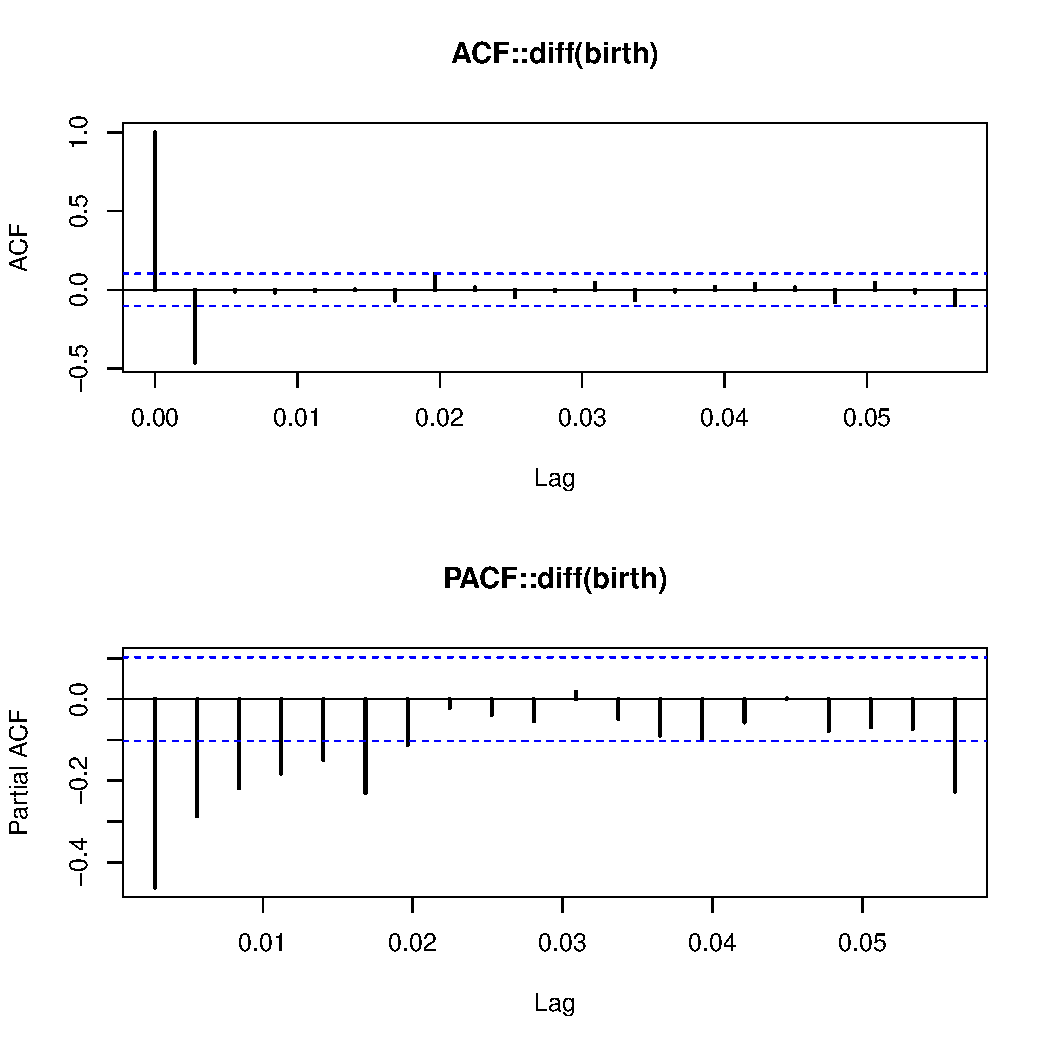
\includegraphics[width=\maxwidth]{figure/unnamed-chunk-9-2} 

\end{knitrout}
From acf plot ,q \leq 1, and from partial-acf plot, p \leq 6 with d = 1

\begin{knitrout}
\definecolor{shadecolor}{rgb}{0.969, 0.969, 0.969}\color{fgcolor}\begin{kframe}
\begin{alltt}
\hlstd{AIC_best} \hlkwb{<-} \hlnum{10}\hlopt{**}\hlnum{6}
\hlkwa{for} \hlstd{(p} \hlkwa{in} \hlnum{0}\hlopt{:}\hlnum{6}\hlstd{)\{}
  \hlkwa{for} \hlstd{(q} \hlkwa{in} \hlnum{0}\hlopt{:}\hlnum{1}\hlstd{)\{}
    \hlstd{fit_arima} \hlkwb{<-} \hlkwd{Arima}\hlstd{(birth_cal,} \hlkwc{order} \hlstd{=} \hlkwd{c}\hlstd{(p,}\hlnum{1}\hlstd{,q))}
    \hlkwa{if} \hlstd{(fit_arima}\hlopt{$}\hlstd{aic} \hlopt{<} \hlstd{AIC_best)\{}
      \hlstd{AIC_best} \hlkwb{<-} \hlstd{fit_arima}\hlopt{$}\hlstd{aic}
      \hlkwd{cat}\hlstd{(}\hlstr{"p = "}\hlstd{,p,}\hlstr{",d = 1, q = "}\hlstd{,q,}\hlstr{", AIC = "}\hlstd{,AIC_best,}\hlstr{"\textbackslash{}n"}\hlstd{)}
    \hlstd{\}}
  \hlstd{\}}
\hlstd{\}}
\end{alltt}
\begin{verbatim}
## p =  0 ,d = 1, q =  0 , AIC =  2648.768 
## p =  0 ,d = 1, q =  1 , AIC =  2462.221 
## p =  1 ,d = 1, q =  1 , AIC =  2459.074
\end{verbatim}
\end{kframe}
\end{knitrout}
ARIMA(1,1,1) has the lowest AIC, so we choose ARIMA(1,1,1)

\begin{knitrout}
\definecolor{shadecolor}{rgb}{0.969, 0.969, 0.969}\color{fgcolor}\begin{kframe}
\begin{alltt}
\hlstd{arima_fit} \hlkwb{<-} \hlkwd{Arima}\hlstd{(birth_cal,}\hlkwc{order} \hlstd{=} \hlkwd{c}\hlstd{(}\hlnum{1}\hlstd{,}\hlnum{1}\hlstd{,}\hlnum{1}\hlstd{))}
\end{alltt}
\end{kframe}
\end{knitrout}

3. Examining the normality of the residuals to test the ARIMA(1,1,1) model
\begin{knitrout}
\definecolor{shadecolor}{rgb}{0.969, 0.969, 0.969}\color{fgcolor}\begin{kframe}
\begin{alltt}
\hlkwd{par}\hlstd{(}\hlkwc{mfrow}\hlstd{=}\hlkwd{c}\hlstd{(}\hlnum{1}\hlstd{,}\hlnum{1}\hlstd{))}
\hlkwd{plot}\hlstd{(}\hlkwd{resid}\hlstd{(arima_fit),}\hlkwc{lwd}\hlstd{=}\hlnum{2}\hlstd{,} \hlkwc{main}\hlstd{=}\hlstr{"resid(ARIMA(1,1,1))"}\hlstd{)}
\end{alltt}
\end{kframe}
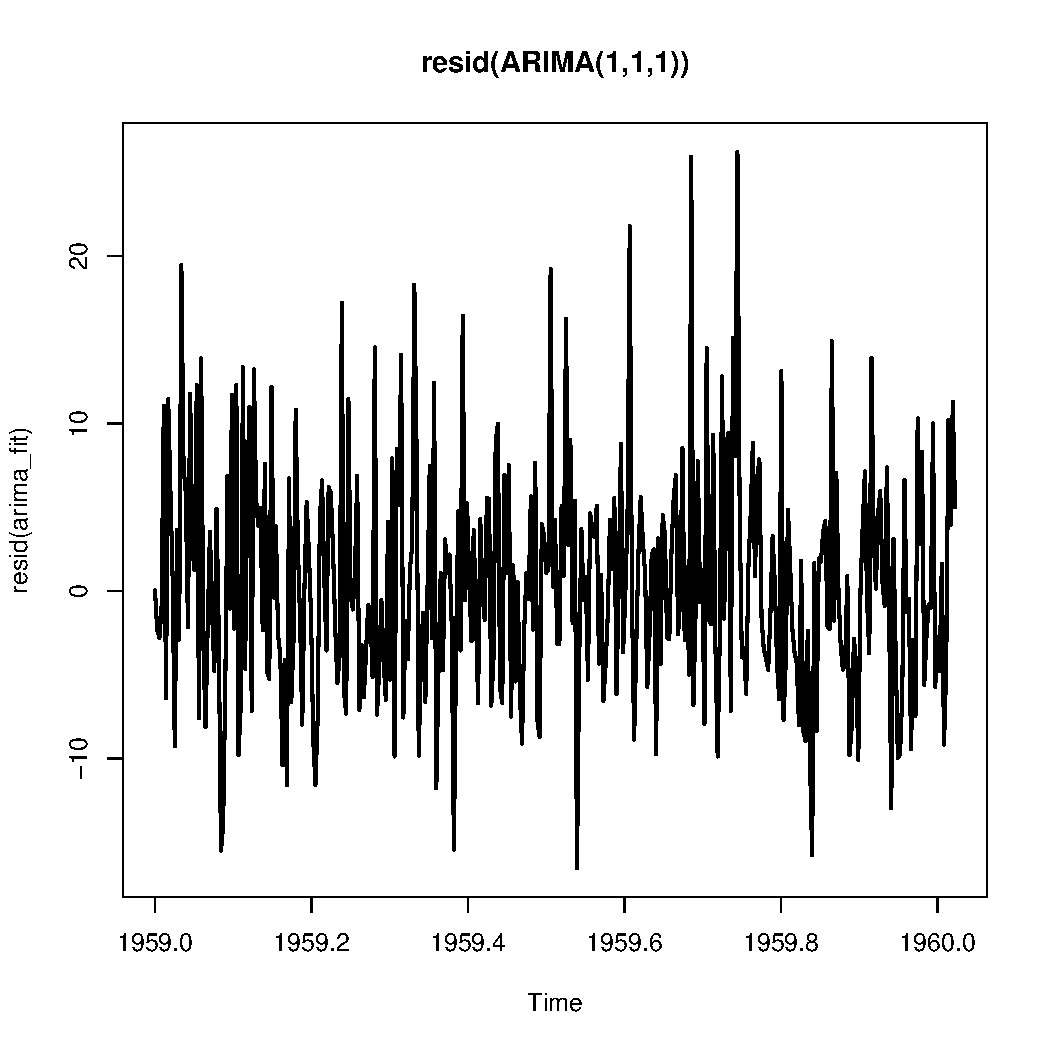
\includegraphics[width=\maxwidth]{figure/unnamed-chunk-12-1} 
\begin{kframe}\begin{alltt}
\hlkwd{par}\hlstd{(}\hlkwc{mfrow}\hlstd{=}\hlkwd{c}\hlstd{(}\hlnum{2}\hlstd{,}\hlnum{1}\hlstd{))}
\hlkwd{acf}\hlstd{(}\hlkwd{resid}\hlstd{(arima_fit),}\hlkwc{lwd}\hlstd{=}\hlnum{2}\hlstd{,} \hlkwc{main}\hlstd{=}\hlstr{"ACF::resid(ARIMA(1,1,1))"}\hlstd{,}\hlkwc{lag.max} \hlstd{=} \hlnum{20}\hlstd{)}
\hlkwd{pacf}\hlstd{(}\hlkwd{resid}\hlstd{(arima_fit),}\hlkwc{lwd}\hlstd{=}\hlnum{2}\hlstd{,} \hlkwc{main}\hlstd{=}\hlstr{"PACF::resid(ARIMA(1,1,1))"}\hlstd{,}\hlkwc{lag.max} \hlstd{=} \hlnum{20}\hlstd{)}
\end{alltt}
\end{kframe}
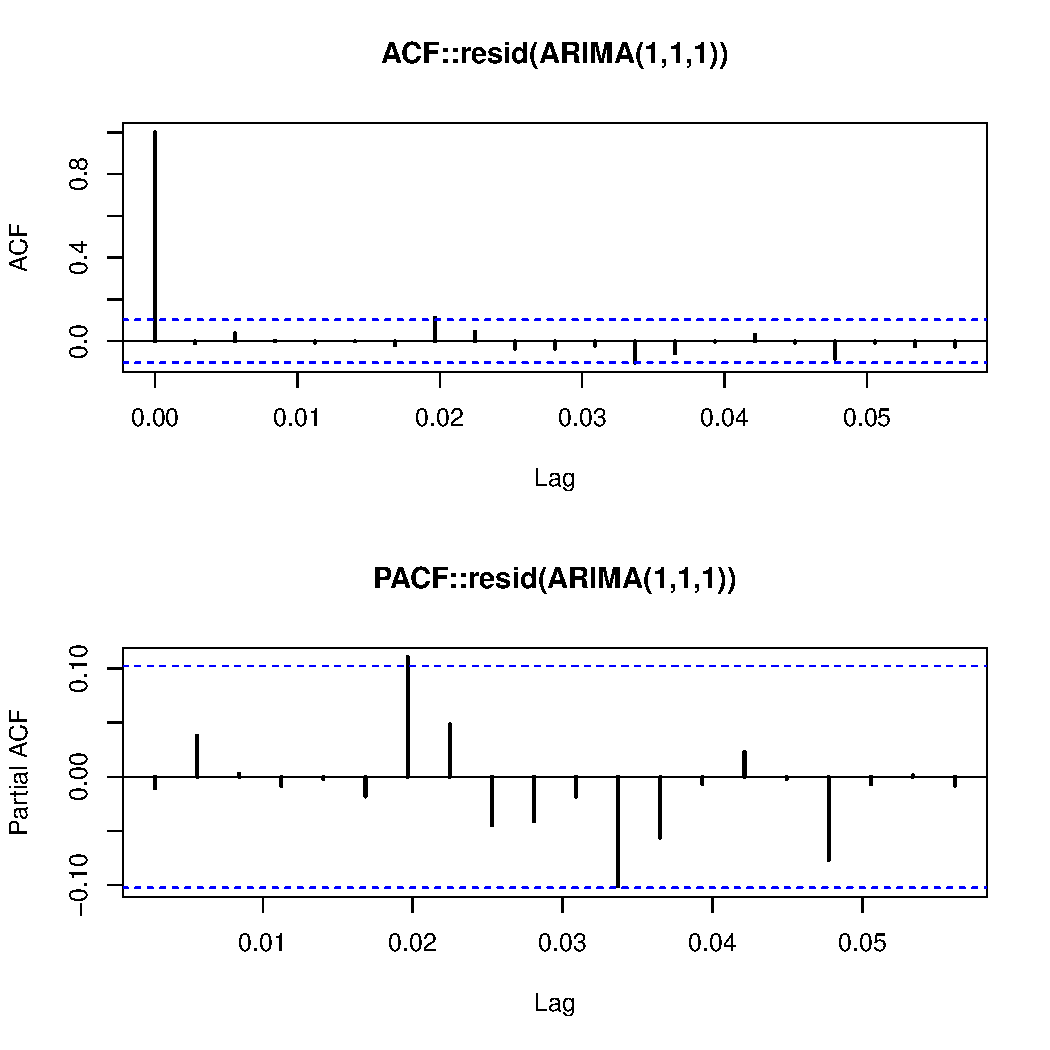
\includegraphics[width=\maxwidth]{figure/unnamed-chunk-12-2} 
\begin{kframe}\begin{alltt}
\hlkwd{par}\hlstd{(}\hlkwc{mfrow}\hlstd{=}\hlkwd{c}\hlstd{(}\hlnum{1}\hlstd{,}\hlnum{1}\hlstd{))}
\hlkwd{qqnorm}\hlstd{(}\hlkwd{resid}\hlstd{(arima_fit),} \hlkwc{main}\hlstd{=}\hlstr{"QQplot::resid(ARIMA(1,1,1))"}\hlstd{,} \hlkwc{lwd}\hlstd{=}\hlnum{3}\hlstd{)}
\hlkwd{qqline}\hlstd{(}\hlkwd{resid}\hlstd{(arima_fit),} \hlkwc{lwd}\hlstd{=}\hlnum{2}\hlstd{,} \hlkwc{col}\hlstd{=}\hlstr{"red"}\hlstd{)}
\end{alltt}
\end{kframe}
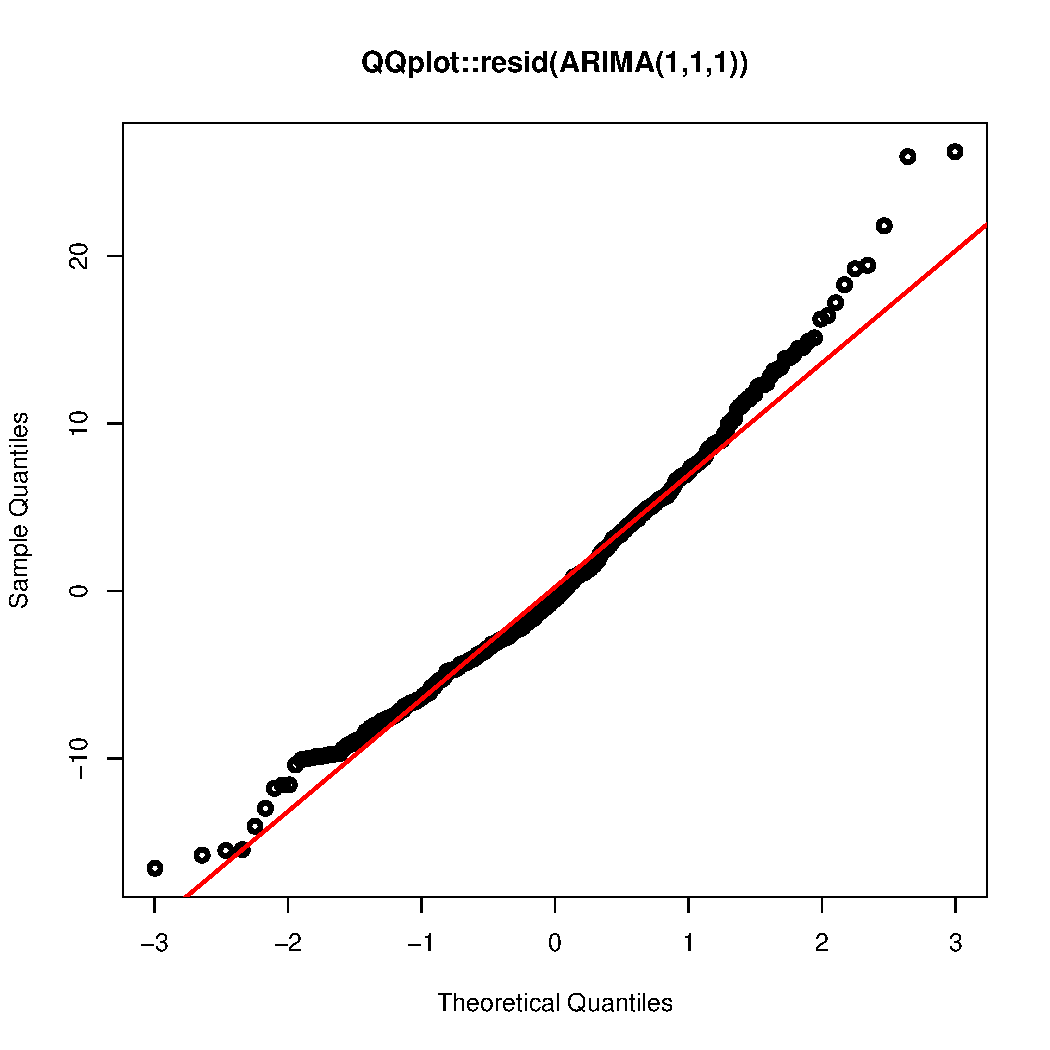
\includegraphics[width=\maxwidth]{figure/unnamed-chunk-12-3} 

\end{knitrout}
Thus, the residuals are follows a Gaussian Distribution.
\bigskip
4. Another model is Double exponential smooting
\begin{knitrout}
\definecolor{shadecolor}{rgb}{0.969, 0.969, 0.969}\color{fgcolor}\begin{kframe}
\begin{alltt}
\hlstd{DES_fit} \hlkwb{<-} \hlkwd{holt}\hlstd{(birth_cal,} \hlkwc{initial} \hlstd{=} \hlstr{"optimal"}\hlstd{,} \hlkwc{h} \hlstd{=}\hlnum{2}\hlopt{*}\hlnum{7}\hlstd{)}
\hlstd{DES_fit}
\end{alltt}
\begin{verbatim}
##           Point Forecast    Lo 80    Hi 80    Lo 95    Hi 95
## 1960.0253       44.29105 35.22863 53.35346 30.43128 58.15081
## 1960.0281       44.31156 35.23049 53.39262 30.42326 58.19985
## 1960.0309       44.33206 35.23232 53.43181 30.41521 58.24892
## 1960.0337       44.35257 35.23414 53.47101 30.40713 58.29802
## 1960.0365       44.37308 35.23593 53.51024 30.39902 58.34715
## 1960.0393       44.39359 35.23771 53.54948 30.39088 58.39631
## 1960.0421       44.41410 35.23947 53.58874 30.38270 58.44550
## 1960.0449       44.43461 35.24120 53.62803 30.37450 58.49472
## 1960.0478       44.45512 35.24292 53.66733 30.36627 58.54397
## 1960.0506       44.47563 35.24462 53.70665 30.35801 58.59325
## 1960.0534       44.49614 35.24630 53.74599 30.34972 58.64256
## 1960.0562       44.51665 35.24795 53.78535 30.34140 58.69190
## 1960.0590       44.53716 35.24959 53.82473 30.33305 58.74127
## 1960.0618       44.55767 35.25121 53.86413 30.32467 58.79067
\end{verbatim}
\begin{alltt}
\hlkwd{plot}\hlstd{(DES_fit,}\hlkwc{main} \hlstd{=} \hlstr{"Birth Forecasts from Double Exponential Smoothing"}\hlstd{,} \hlkwc{lwd} \hlstd{=} \hlnum{2}\hlstd{)}
\end{alltt}
\end{kframe}
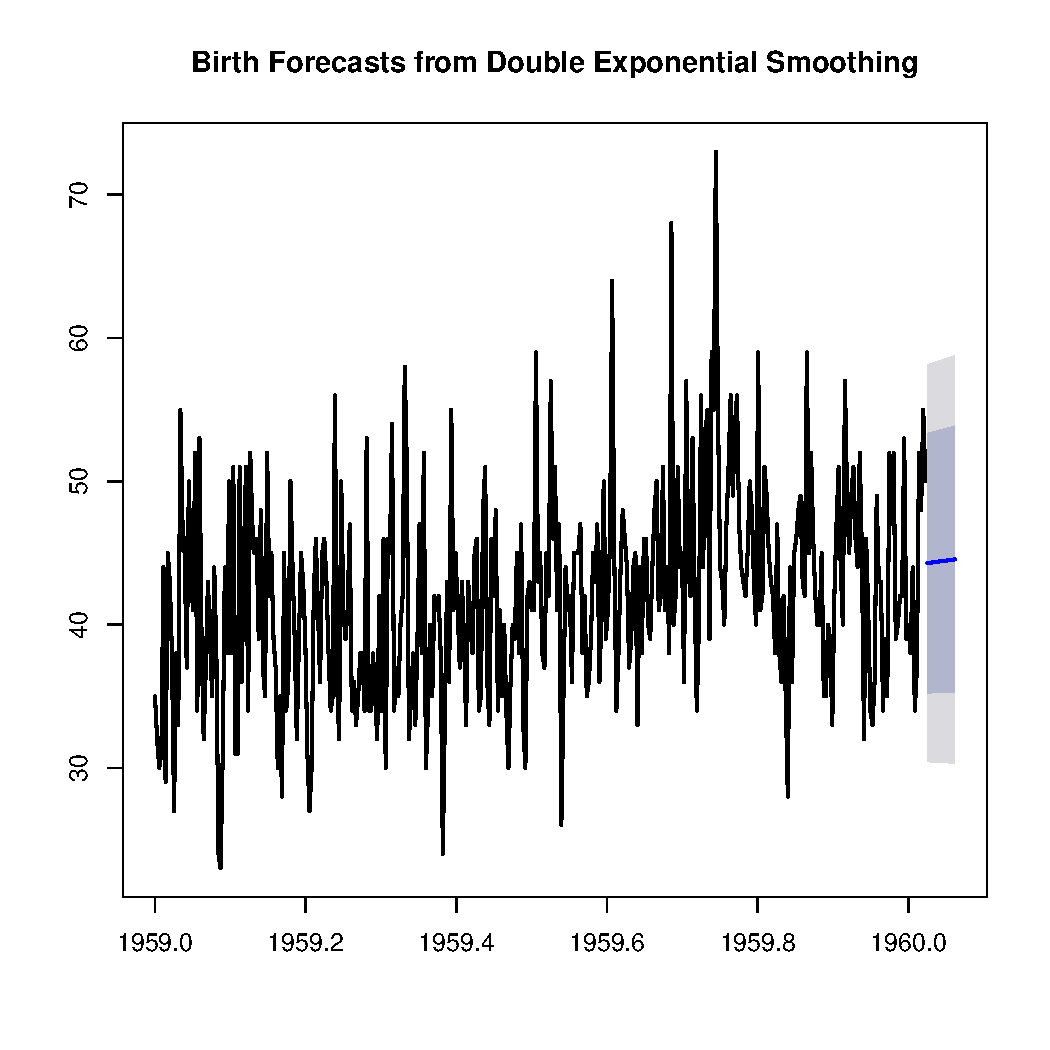
\includegraphics[width=\maxwidth]{figure/unnamed-chunk-13-1} 

\end{knitrout}

5. Compare ARIMA(1,1,1) and DES by using cross-validation
\begin{knitrout}
\definecolor{shadecolor}{rgb}{0.969, 0.969, 0.969}\color{fgcolor}\begin{kframe}
\begin{alltt}
\hlcom{#Define a function CV to do cross-validation}
\hlstd{CV} \hlkwb{<-}  \hlkwa{function}\hlstd{(}\hlkwc{time_series}\hlstd{,} \hlkwc{start}\hlstd{,} \hlkwc{forecast_length}\hlstd{,}\hlkwc{ts_model}\hlstd{)\{}
  \hlstd{ts_length} \hlkwb{<-}  \hlkwd{length}\hlstd{(time_series)}
  \hlstd{accuracy_list} \hlkwb{=} \hlkwd{c}\hlstd{()}
  \hlkwa{for}\hlstd{(k} \hlkwa{in} \hlstd{start}\hlopt{:}\hlstd{(ts_length} \hlopt{-} \hlstd{forecast_length))\{}
    \hlstd{fitted_model} \hlkwb{<-} \hlkwd{ts_model}\hlstd{(}\hlkwd{ts}\hlstd{(time_series[}\hlnum{0}\hlopt{:}\hlstd{k]))}
    \hlstd{RMSE} \hlkwb{<-}  \hlkwd{accuracy}\hlstd{(}\hlkwd{forecast}\hlstd{(fitted_model,} \hlkwc{h} \hlstd{= forecast_length))[}\hlnum{2}\hlstd{]}
    \hlstd{accuracy_list} \hlkwb{=} \hlkwd{c}\hlstd{(accuracy_list, RMSE)}
  \hlstd{\}}
  \hlkwd{return}\hlstd{(accuracy_list)}
\hlstd{\}}

\hlcom{#Define two models}
\hlstd{model_ARIMA} \hlkwb{<-} \hlkwa{function}\hlstd{(}\hlkwc{ts}\hlstd{)} \hlkwd{return}\hlstd{(}\hlkwd{Arima}\hlstd{(ts,}\hlkwc{order} \hlstd{=} \hlkwd{c}\hlstd{(}\hlnum{1}\hlstd{,}\hlnum{1}\hlstd{,}\hlnum{1}\hlstd{)))}
\hlstd{model_DES} \hlkwb{<-} \hlkwa{function}\hlstd{(}\hlkwc{ts}\hlstd{)} \hlkwd{return}\hlstd{(}\hlkwd{holt}\hlstd{(ts,}\hlkwc{initial} \hlstd{=} \hlstr{"optimal"}\hlstd{))}

\hlstd{start} \hlkwb{<-} \hlnum{250}
\hlstd{forecast_length} \hlkwb{<-} \hlnum{7}
\hlstd{CV_birth_Cal} \hlkwb{<-} \hlkwd{data.frame}\hlstd{(}
  \hlkwc{arima} \hlstd{=} \hlkwd{CV}\hlstd{(birth_cal, start, forecast_length, model_ARIMA),}
  \hlkwc{des} \hlstd{=} \hlkwd{CV}\hlstd{(birth_cal, start, forecast_length, model_DES)}
\hlstd{)}

\hlkwd{boxplot}\hlstd{(CV_birth_Cal,}\hlkwc{main} \hlstd{=} \hlstr{"Birth::Cross Validation for RMSE"}\hlstd{,} \hlkwc{lwd}\hlstd{=}\hlnum{2}\hlstd{)}
\end{alltt}
\end{kframe}
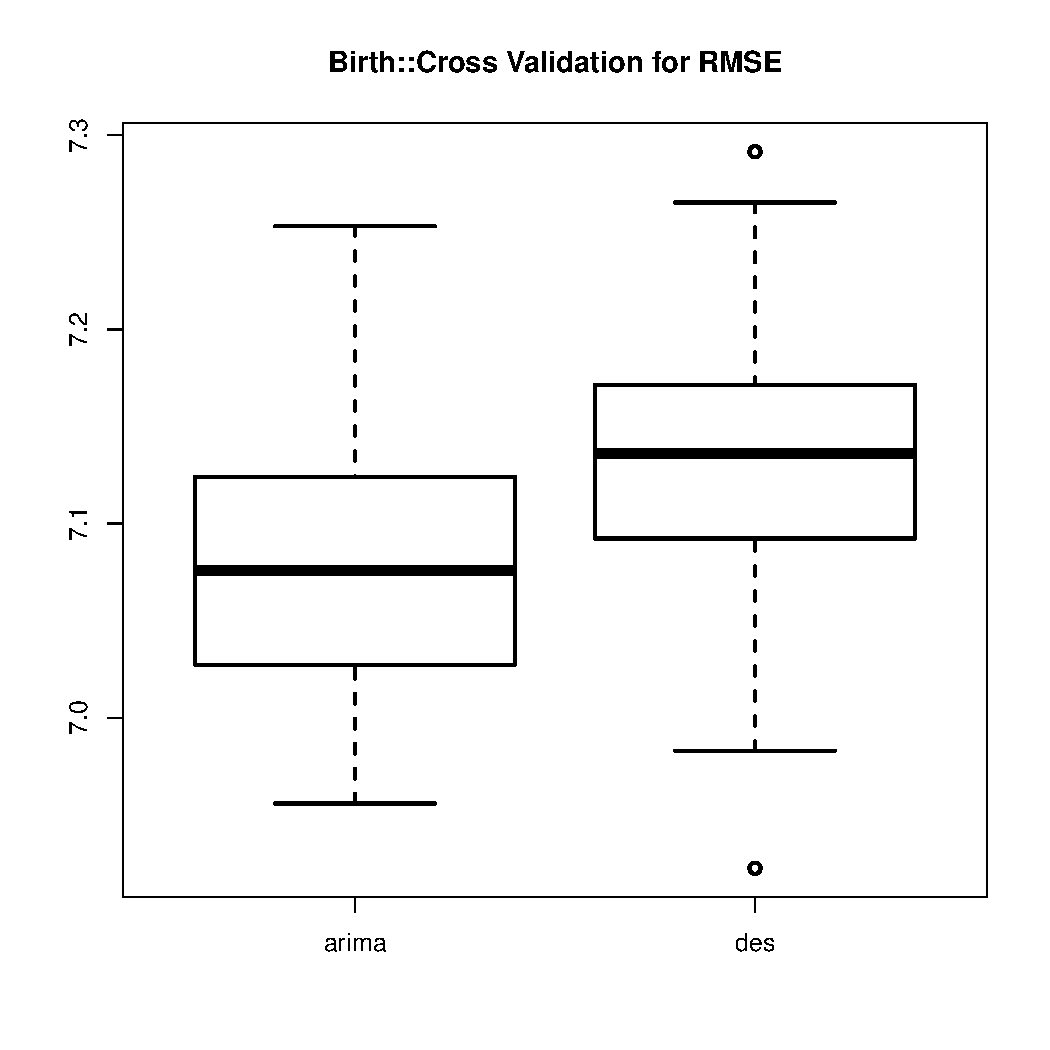
\includegraphics[width=\maxwidth]{figure/unnamed-chunk-14-1} 

\end{knitrout}

From boxplot, ARIMA(1,1,1) has a lower RMSE, which is a better model. That's why we choose ARIMA(1,1,1)
\bigskip
6. Forecast the number of birth during the two weeks by using ARIMA(1,1,1)
\begin{knitrout}
\definecolor{shadecolor}{rgb}{0.969, 0.969, 0.969}\color{fgcolor}\begin{kframe}
\begin{alltt}
\hlstd{arima_forecast} \hlkwb{<-} \hlkwd{forecast}\hlstd{(arima_fit,} \hlkwc{h} \hlstd{=} \hlnum{2}\hlopt{*}\hlnum{7}\hlstd{)}
\hlstd{arima_forecast}
\end{alltt}
\begin{verbatim}
##           Point Forecast    Lo 80    Hi 80    Lo 95    Hi 95
## 1960.0253       44.55357 35.54440 53.56275 30.77523 58.33191
## 1960.0281       43.87142 34.74366 52.99918 29.91172 57.83113
## 1960.0309       43.78599 34.64332 52.92865 29.80348 57.76849
## 1960.0337       43.77528 34.62372 52.92685 29.77917 57.77140
## 1960.0365       43.77394 34.61412 52.93376 29.76521 57.78268
## 1960.0393       43.77378 34.60579 52.94176 29.75255 57.79500
## 1960.0421       43.77376 34.59762 52.94989 29.74007 57.80744
## 1960.0449       43.77375 34.58948 52.95803 29.72761 57.81989
## 1960.0478       43.77375 34.58134 52.96616 29.71517 57.83233
## 1960.0506       43.77375 34.57322 52.97429 29.70275 57.84476
## 1960.0534       43.77375 34.56510 52.98241 29.69033 57.85718
## 1960.0562       43.77375 34.55699 52.99052 29.67792 57.86958
## 1960.0590       43.77375 34.54888 52.99862 29.66553 57.88198
## 1960.0618       43.77375 34.54078 53.00672 29.65314 57.89436
\end{verbatim}
\begin{alltt}
\hlkwd{plot}\hlstd{(arima_forecast,}\hlkwc{main} \hlstd{=} \hlstr{"Birth Forecasts from ARIMA(1,1,1)"}\hlstd{,}\hlkwc{lwd} \hlstd{=} \hlnum{2}\hlstd{)}
\end{alltt}
\end{kframe}
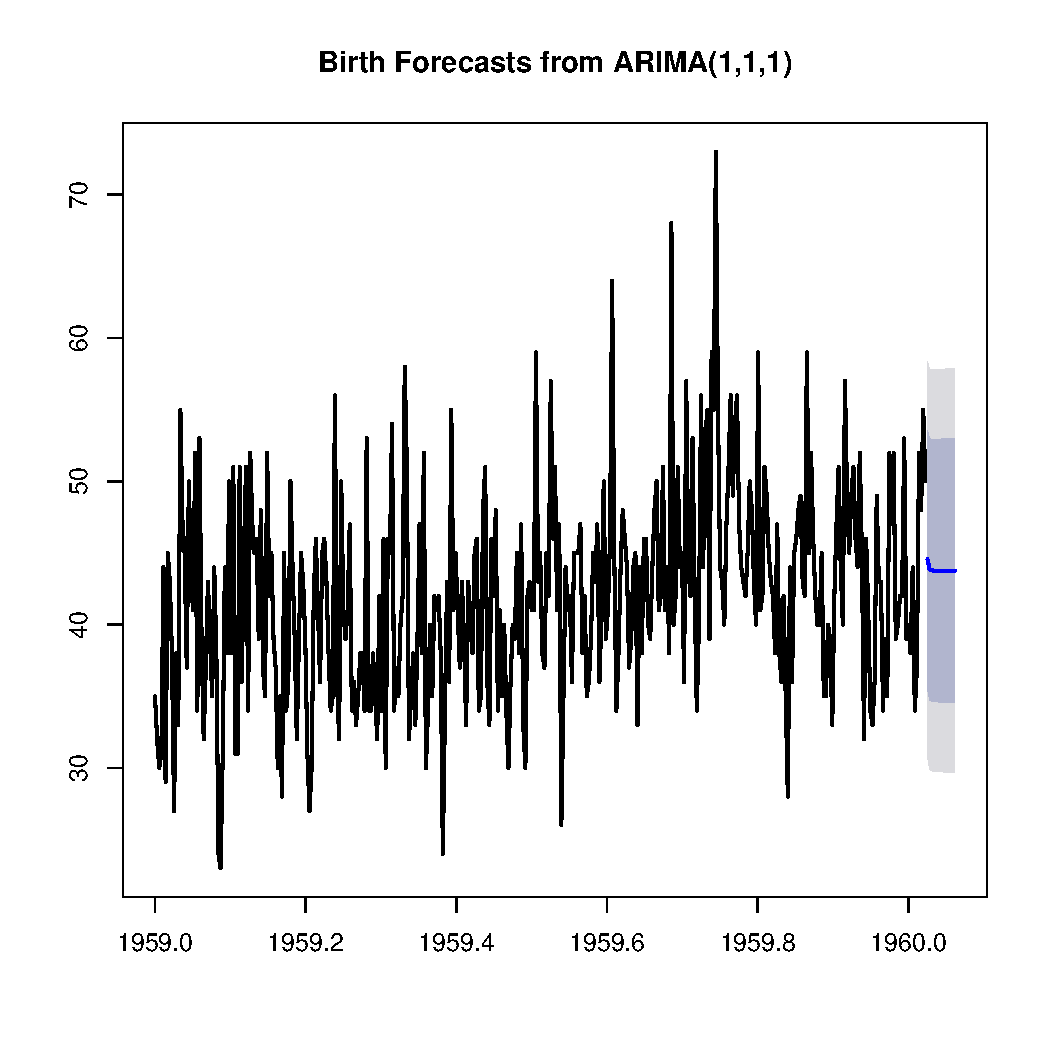
\includegraphics[width=\maxwidth]{figure/unnamed-chunk-15-1} 

\end{knitrout}


\section{ Exercise 3 (How much beer?)}

1. Load the data and plot.
\begin{knitrout}
\definecolor{shadecolor}{rgb}{0.969, 0.969, 0.969}\color{fgcolor}\begin{kframe}
\begin{alltt}
\hlstd{beer_data} \hlkwb{<-} \hlkwd{read.csv}\hlstd{(}\hlstr{"E:/ST3233/Assignment2/Datasets/quarterly-beer-production-in-aus.csv"}\hlstd{,}
                      \hlkwc{header}\hlstd{=} \hlnum{TRUE}\hlstd{,}\hlkwc{sep}\hlstd{=}\hlstr{","}\hlstd{)}
\hlstd{beer} \hlkwb{<-} \hlkwd{ts}\hlstd{(beer_data}\hlopt{$}\hlstd{beer_production,}\hlkwc{frequency} \hlstd{=} \hlnum{4}\hlstd{,}\hlkwc{start}\hlstd{=}\hlkwd{c}\hlstd{(}\hlnum{1956}\hlstd{))}
\hlkwd{par}\hlstd{(}\hlkwc{mfrow}\hlstd{=}\hlkwd{c}\hlstd{(}\hlnum{1}\hlstd{,}\hlnum{1}\hlstd{))}
\hlkwd{plot}\hlstd{(beer,}\hlkwc{lwd} \hlstd{=} \hlnum{2}\hlstd{,} \hlkwc{main} \hlstd{=} \hlstr{"Quarterly Beer Production in Austrilia"}\hlstd{)}
\end{alltt}
\end{kframe}
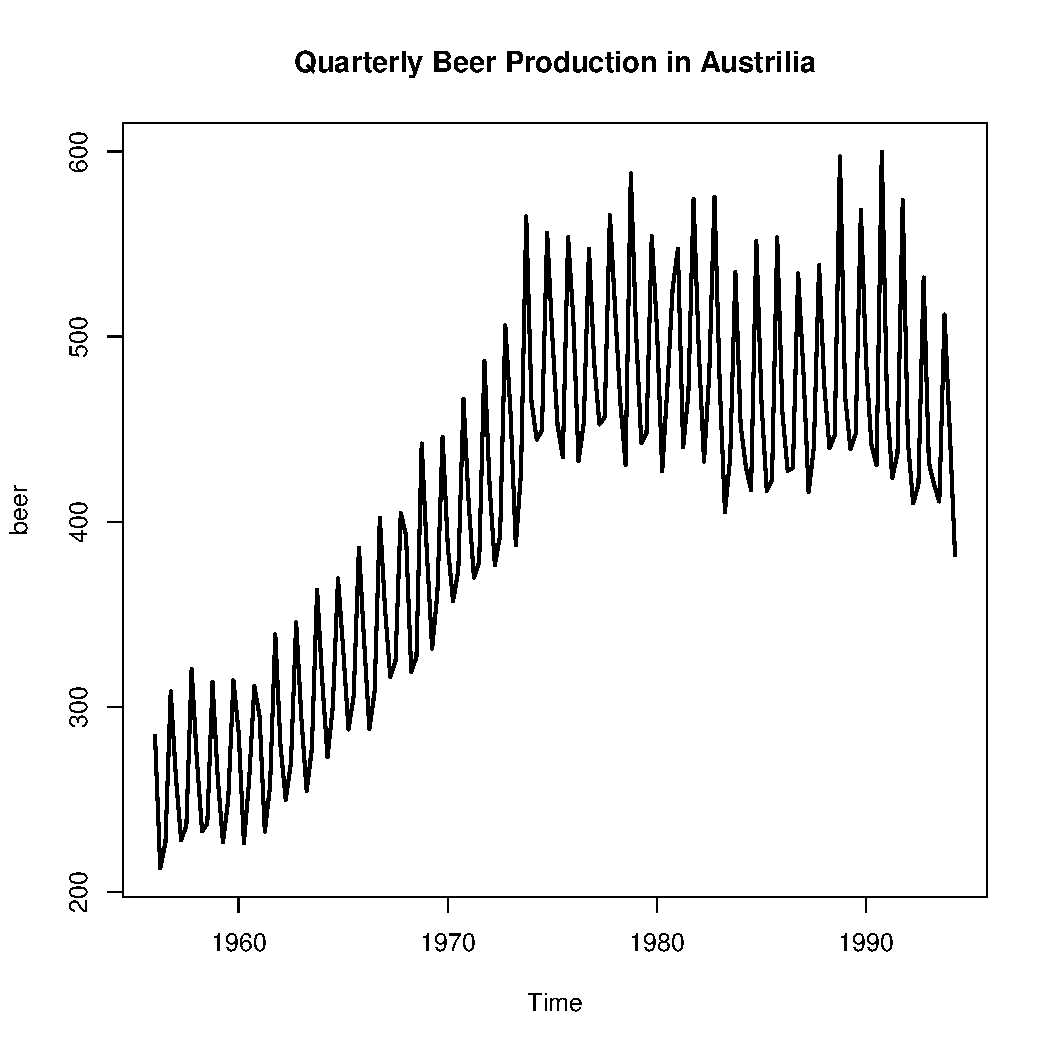
\includegraphics[width=\maxwidth]{figure/unnamed-chunk-16-1} 
\begin{kframe}\begin{alltt}
\hlcom{#From the plot, we can clearly see that there is periodicity and trend, thus we decompose it.}
\hlstd{beer_decmp} \hlkwb{<-}\hlkwd{stl}\hlstd{(beer,}\hlkwc{s.window} \hlstd{=} \hlstr{"periodic"}\hlstd{,} \hlkwc{robust} \hlstd{= T)}
\hlkwd{plot}\hlstd{(beer_decmp)}
\end{alltt}
\end{kframe}
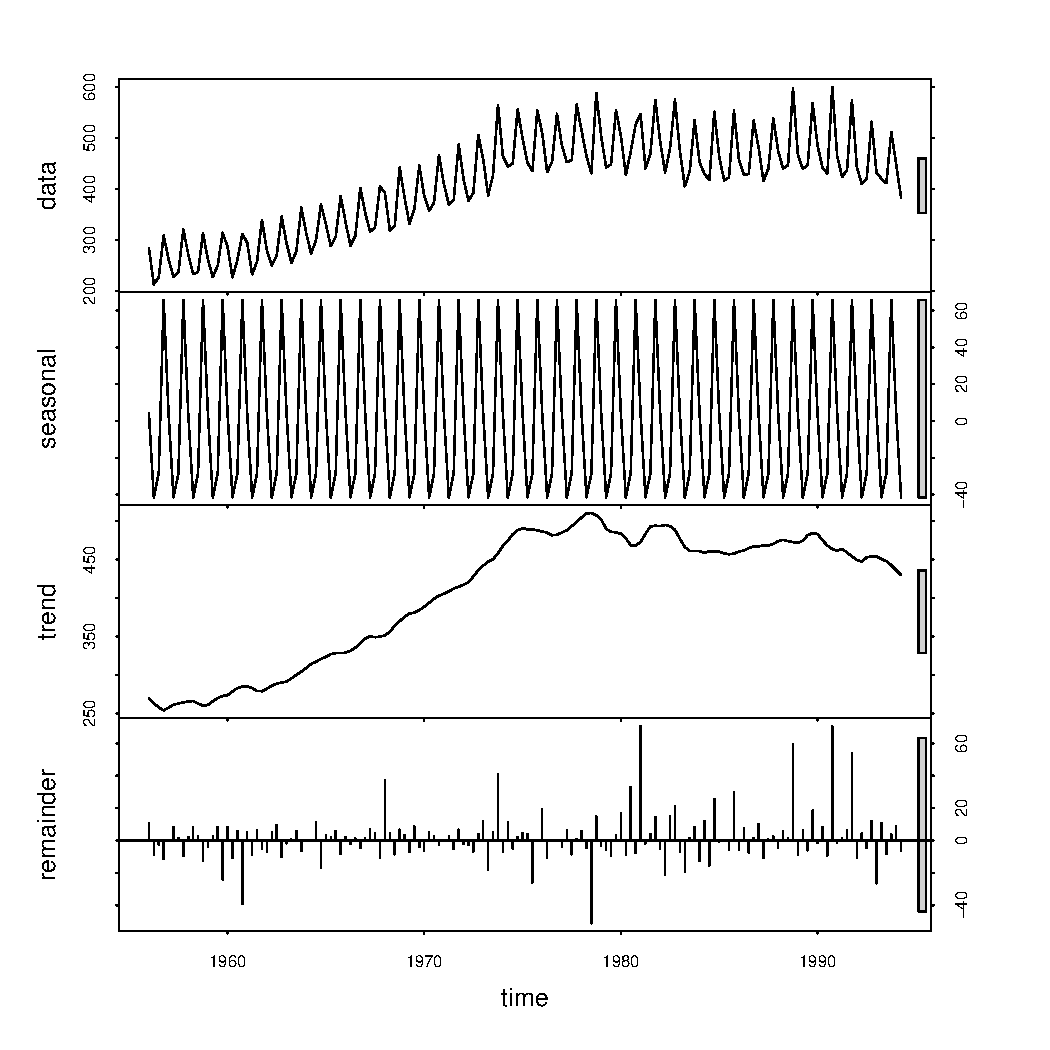
\includegraphics[width=\maxwidth]{figure/unnamed-chunk-16-2} 
\begin{kframe}\begin{alltt}
\hlcom{#seasonal plot}
\hlkwd{seasonplot}\hlstd{(beer} \hlopt{-} \hlstd{beer_decmp}\hlopt{$}\hlstd{time.series[,}\hlstr{"trend"}\hlstd{],} \hlkwc{s} \hlstd{=} \hlnum{4}\hlstd{,}\hlkwc{col} \hlstd{=} \hlnum{1}\hlopt{:}\hlnum{6}\hlstd{,} \hlkwc{type} \hlstd{=} \hlstr{"l"}\hlstd{)}
\end{alltt}
\end{kframe}
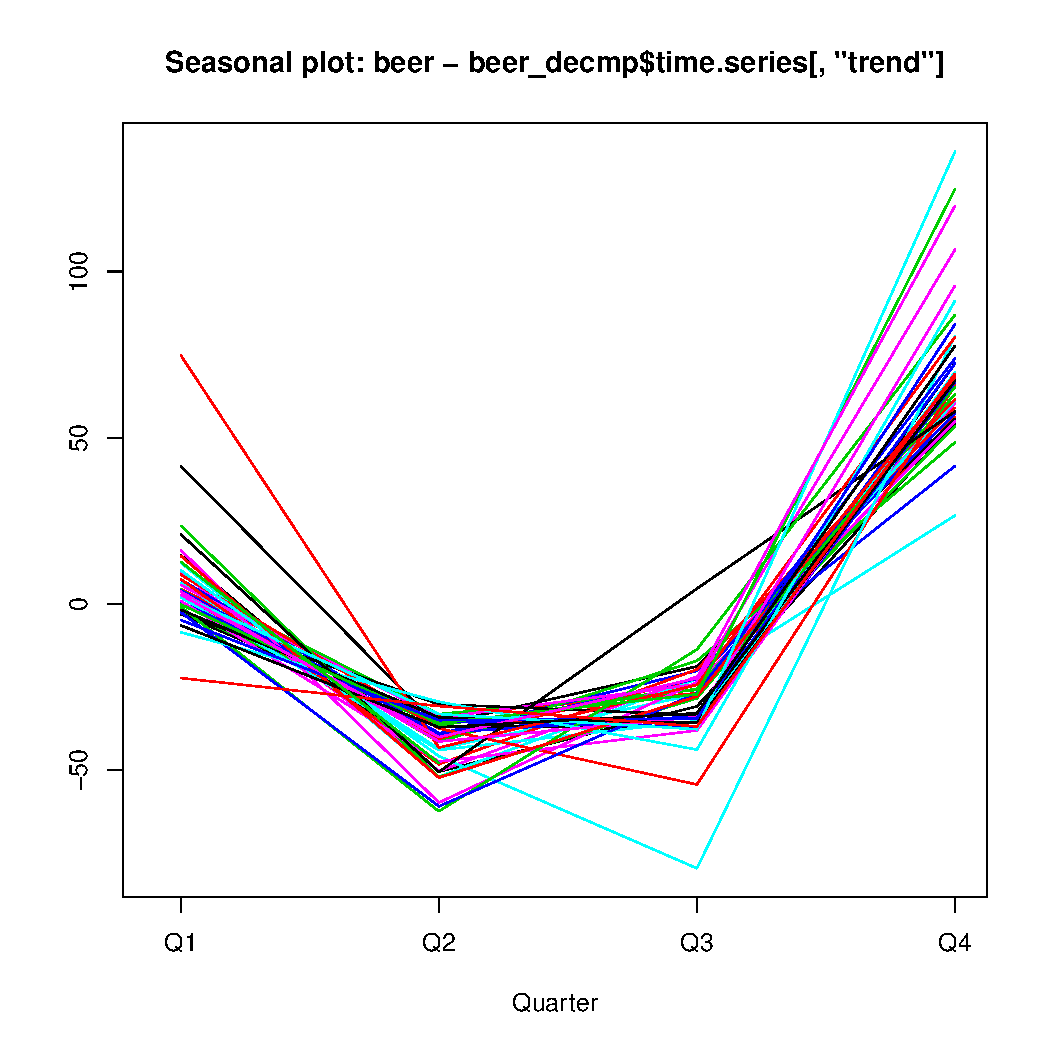
\includegraphics[width=\maxwidth]{figure/unnamed-chunk-16-3} 

\end{knitrout}
There is seasonal behavior, thus we first use SARIMA model
\bigskip
2. Fit the model.
Notice that the fluctation of the time series becomes larger as the time changes, so we consider a new time series: log(beer)

\begin{knitrout}
\definecolor{shadecolor}{rgb}{0.969, 0.969, 0.969}\color{fgcolor}\begin{kframe}
\begin{alltt}
\hlstd{log_beer} \hlkwb{=} \hlkwd{log}\hlstd{(beer)}
\hlkwd{plot}\hlstd{(log_beer,} \hlkwc{lwd}\hlstd{=}\hlnum{2}\hlstd{,} \hlkwc{main}\hlstd{=}\hlstr{"log_beer"}\hlstd{)}
\end{alltt}
\end{kframe}
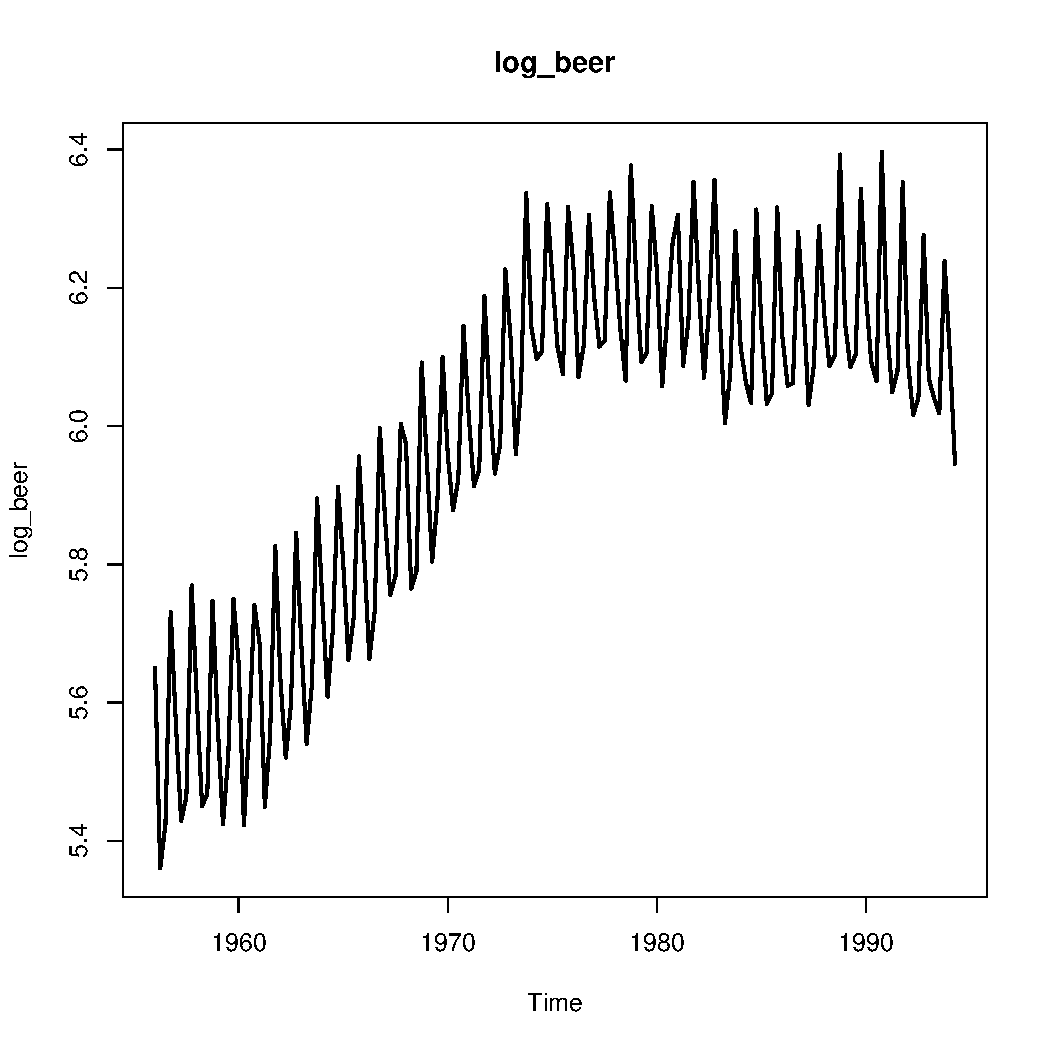
\includegraphics[width=\maxwidth]{figure/unnamed-chunk-17-1} 
\begin{kframe}\begin{alltt}
\hlstd{log_beer_d4} \hlkwb{=} \hlkwd{diff}\hlstd{(log_beer,} \hlkwc{lag} \hlstd{=} \hlnum{4}\hlstd{)}
\hlkwd{plot}\hlstd{(log_beer_d4,}\hlkwc{lwd} \hlstd{=} \hlnum{2}\hlstd{,} \hlkwc{main} \hlstd{=} \hlstr{"diff(log_beer, lag = 4)"}\hlstd{)}
\end{alltt}
\end{kframe}
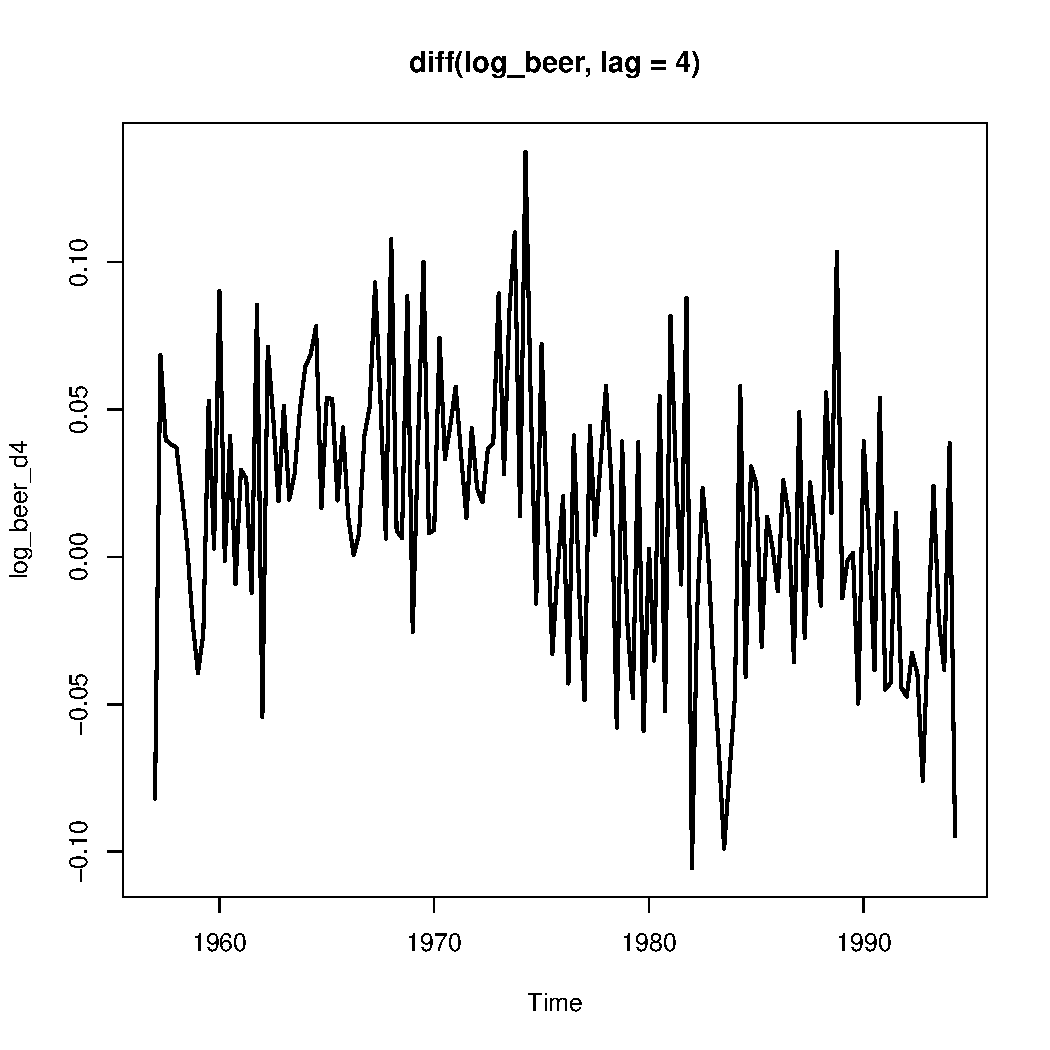
\includegraphics[width=\maxwidth]{figure/unnamed-chunk-17-2} 
\begin{kframe}\begin{alltt}
\hlstd{log_beer_d4_d1} \hlkwb{=} \hlkwd{diff}\hlstd{(log_beer_d4,} \hlkwc{lag} \hlstd{=} \hlnum{1}\hlstd{)}
\hlkwd{plot}\hlstd{(log_beer_d4_d1,}\hlkwc{lwd} \hlstd{=} \hlnum{2}\hlstd{,} \hlkwc{main} \hlstd{=} \hlstr{"diff(diff(log_beer, lag = 4))"}\hlstd{)}
\end{alltt}
\end{kframe}
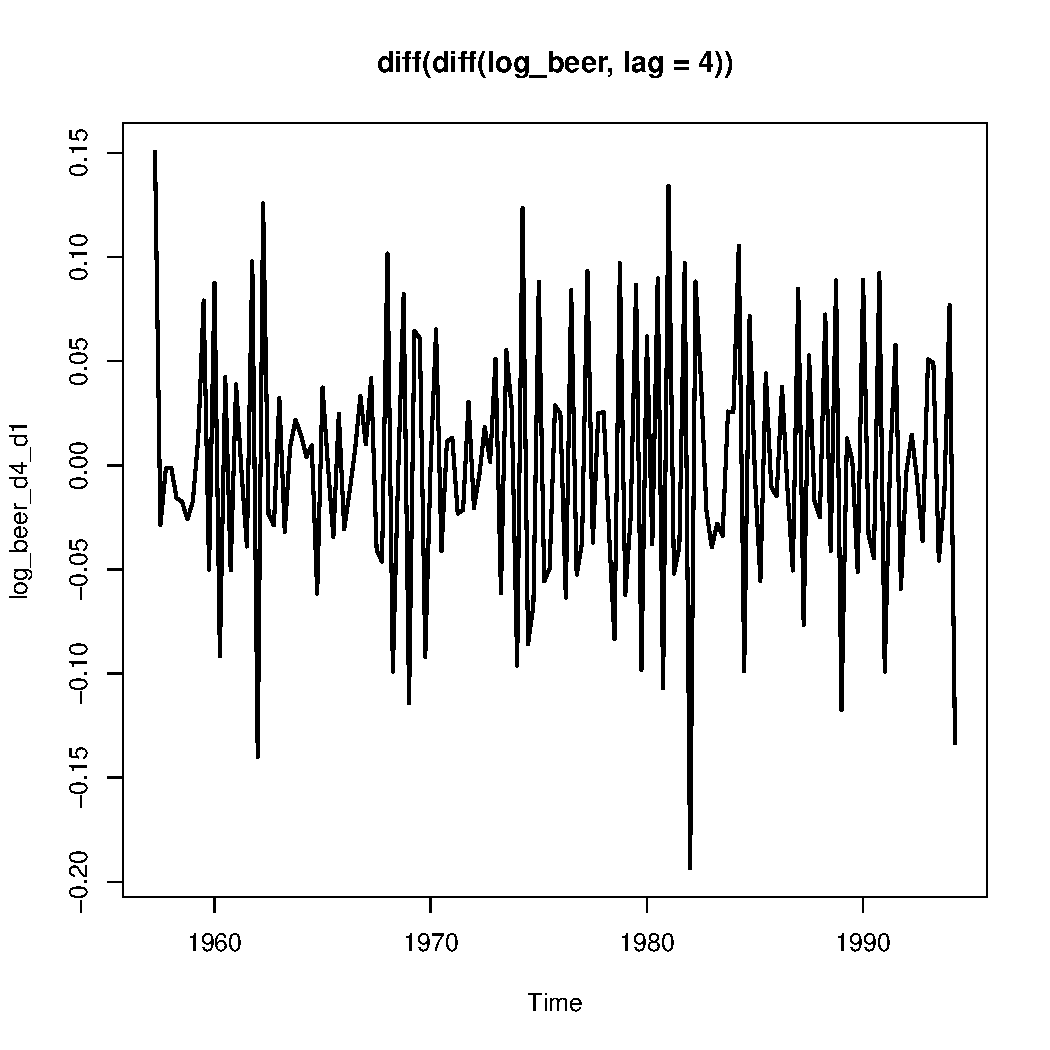
\includegraphics[width=\maxwidth]{figure/unnamed-chunk-17-3} 
\begin{kframe}\begin{alltt}
\hlkwd{par}\hlstd{(}\hlkwc{mfrow}\hlstd{=}\hlkwd{c}\hlstd{(}\hlnum{2}\hlstd{,}\hlnum{1}\hlstd{))}
\hlkwd{acf}\hlstd{(log_beer_d4_d1,}\hlkwc{lwd} \hlstd{=} \hlnum{2}\hlstd{,} \hlkwc{main} \hlstd{=} \hlstr{"ACF::diff(diff(log_beer, lag = 4))"}\hlstd{,}\hlkwc{lag.max} \hlstd{=} \hlnum{20}\hlstd{)}
\hlkwd{pacf}\hlstd{(log_beer_d4_d1,}\hlkwc{lwd} \hlstd{=} \hlnum{2}\hlstd{,} \hlkwc{main} \hlstd{=} \hlstr{"PACF::diff(diff(log_beer, lag = 4))"}\hlstd{,}\hlkwc{lag.max} \hlstd{=} \hlnum{20}\hlstd{)}
\end{alltt}
\end{kframe}
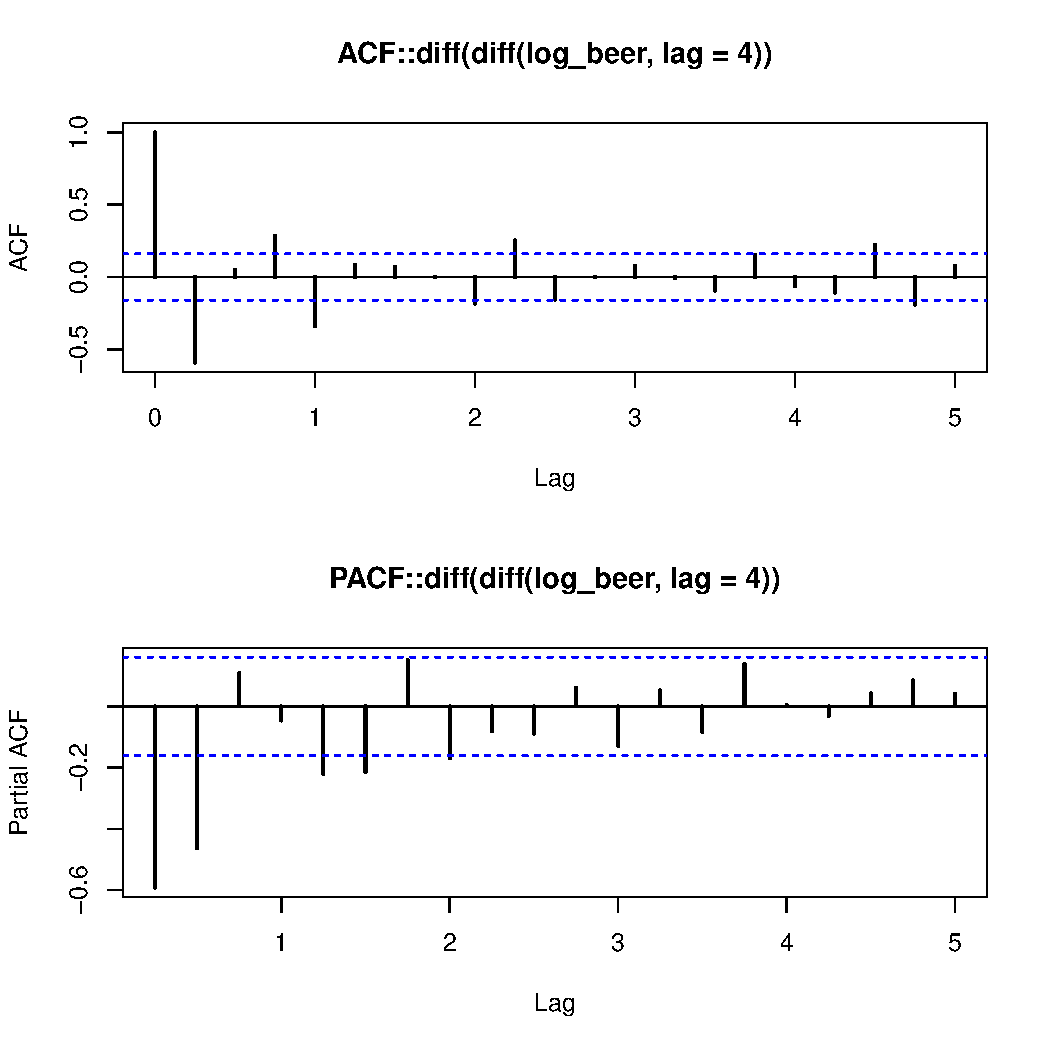
\includegraphics[width=\maxwidth]{figure/unnamed-chunk-17-4} 

\end{knitrout}
From acf plot ,q \leq 4, and from partial-acf plot, p \leq 2 with d = D = 1 and P \leq 1, Q \leq 1

\begin{knitrout}
\definecolor{shadecolor}{rgb}{0.969, 0.969, 0.969}\color{fgcolor}\begin{kframe}
\begin{alltt}
\hlstd{AIC_best} \hlkwb{<-} \hlnum{10}\hlopt{**}\hlnum{6}
\hlkwa{for} \hlstd{(p} \hlkwa{in} \hlnum{0}\hlopt{:}\hlnum{2}\hlstd{)\{}
  \hlkwa{for} \hlstd{(q} \hlkwa{in} \hlnum{0}\hlopt{:}\hlnum{4}\hlstd{)\{}
    \hlkwa{for} \hlstd{(P} \hlkwa{in} \hlnum{0}\hlopt{:}\hlnum{1}\hlstd{)\{}
      \hlkwa{for} \hlstd{(Q} \hlkwa{in} \hlnum{0}\hlopt{:}\hlnum{1}\hlstd{)\{}
        \hlstd{fit_sarima} \hlkwb{<-} \hlkwd{Arima}\hlstd{(log_beer,} \hlkwc{order} \hlstd{=} \hlkwd{c}\hlstd{(p,}\hlnum{1}\hlstd{,q),} \hlkwc{seasonal} \hlstd{=} \hlkwd{c}\hlstd{(P,}\hlnum{1}\hlstd{,Q))}
        \hlkwa{if} \hlstd{(fit_sarima}\hlopt{$}\hlstd{aic} \hlopt{<} \hlstd{AIC_best)\{}
          \hlstd{AIC_best} \hlkwb{<-} \hlstd{fit_sarima}\hlopt{$}\hlstd{aic}
          \hlkwd{cat}\hlstd{(}\hlstr{"p = "}\hlstd{,p,}\hlstr{", q = "}\hlstd{,q,}\hlstr{",P = "}\hlstd{,P,}\hlstr{",Q = "}\hlstd{,Q,}\hlstr{"\textbackslash{}t AIC = "}\hlstd{,AIC_best,}\hlstr{"\textbackslash{}n"}\hlstd{)}
        \hlstd{\}}
      \hlstd{\}}
    \hlstd{\}}
  \hlstd{\}}
\hlstd{\}}
\end{alltt}
\begin{verbatim}
## p =  0 , q =  0 ,P =  0 ,Q =  0 	 AIC =  -403.1997 
## p =  0 , q =  0 ,P =  0 ,Q =  1 	 AIC =  -456.3742 
## p =  0 , q =  1 ,P =  0 ,Q =  0 	 AIC =  -505.6392 
## p =  0 , q =  1 ,P =  0 ,Q =  1 	 AIC =  -537.6958 
## p =  0 , q =  2 ,P =  0 ,Q =  1 	 AIC =  -556.2169
\end{verbatim}
\end{kframe}
\end{knitrout}
The lowest AIC gives the best fitted model of log_beer, which is SARIMA(0,1,2)(0,1,1)[4]
\begin{knitrout}
\definecolor{shadecolor}{rgb}{0.969, 0.969, 0.969}\color{fgcolor}\begin{kframe}
\begin{alltt}
\hlstd{sarima_fit} \hlkwb{<-} \hlkwd{Arima}\hlstd{(log_beer,} \hlkwc{order} \hlstd{=} \hlkwd{c}\hlstd{(}\hlnum{0}\hlstd{,}\hlnum{1}\hlstd{,}\hlnum{2}\hlstd{),} \hlkwc{seasonal} \hlstd{=} \hlkwd{c}\hlstd{(}\hlnum{0}\hlstd{,}\hlnum{1}\hlstd{,}\hlnum{1}\hlstd{))}
\end{alltt}
\end{kframe}
\end{knitrout}

3. Then consider the residuals of the SARIMA model.
\begin{knitrout}
\definecolor{shadecolor}{rgb}{0.969, 0.969, 0.969}\color{fgcolor}\begin{kframe}
\begin{alltt}
\hlkwd{par}\hlstd{(}\hlkwc{mfrow}\hlstd{=}\hlkwd{c}\hlstd{(}\hlnum{1}\hlstd{,}\hlnum{1}\hlstd{))}
\hlkwd{plot}\hlstd{(}\hlkwd{resid}\hlstd{(sarima_fit),}\hlkwc{lwd}\hlstd{=}\hlnum{2}\hlstd{,} \hlkwc{main}\hlstd{=}\hlstr{"resid(SARIMA(0,1,2)(0,1,1)[4])"}\hlstd{)}
\end{alltt}
\end{kframe}
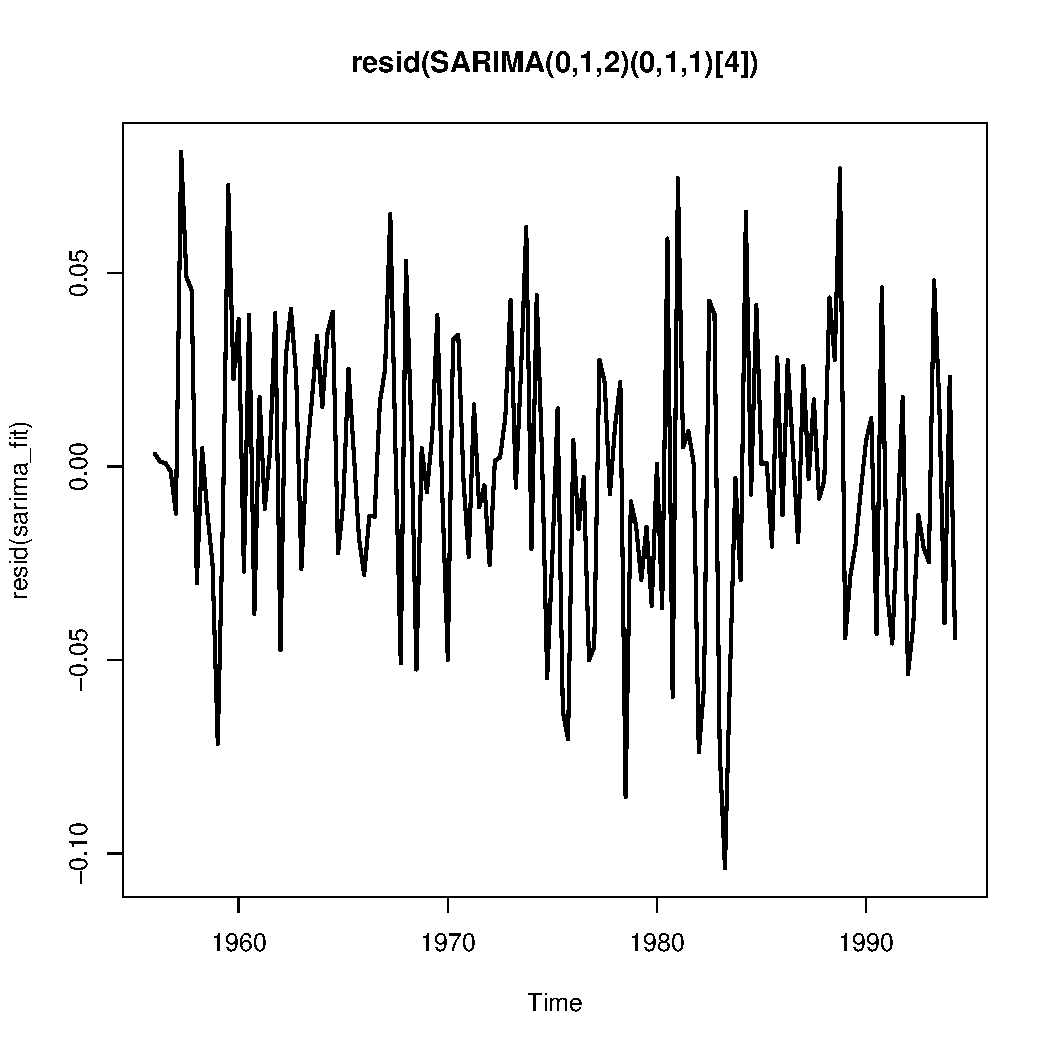
\includegraphics[width=\maxwidth]{figure/unnamed-chunk-20-1} 
\begin{kframe}\begin{alltt}
\hlkwd{par}\hlstd{(}\hlkwc{mfrow}\hlstd{=}\hlkwd{c}\hlstd{(}\hlnum{2}\hlstd{,}\hlnum{1}\hlstd{))}
\hlkwd{acf}\hlstd{(}\hlkwd{resid}\hlstd{(sarima_fit),}\hlkwc{lwd}\hlstd{=}\hlnum{2}\hlstd{,} \hlkwc{main}\hlstd{=}\hlstr{"ACF::resid(SARIMA(0,1,2)(0,1,1)[4])"}\hlstd{)}
\hlkwd{pacf}\hlstd{(}\hlkwd{resid}\hlstd{(sarima_fit),}\hlkwc{lwd}\hlstd{=}\hlnum{2}\hlstd{,} \hlkwc{main}\hlstd{=}\hlstr{"PACF::resid(SARIMA(0,1,2)(0,1,1)[4])"}\hlstd{)}
\end{alltt}
\end{kframe}
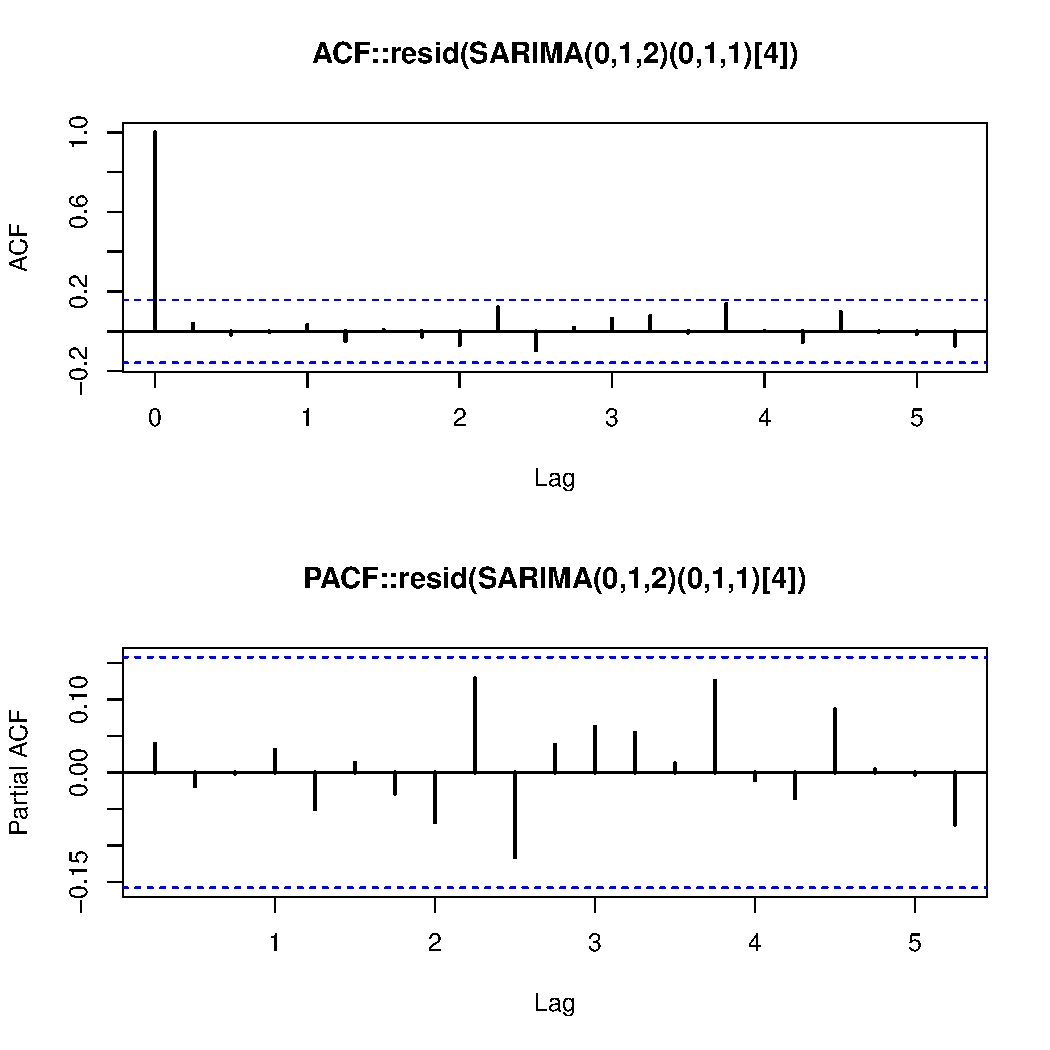
\includegraphics[width=\maxwidth]{figure/unnamed-chunk-20-2} 
\begin{kframe}\begin{alltt}
\hlcom{#The residual is stationary.}

\hlkwd{par}\hlstd{(}\hlkwc{mfrow}\hlstd{=}\hlkwd{c}\hlstd{(}\hlnum{1}\hlstd{,}\hlnum{1}\hlstd{))}
\hlkwd{qqnorm}\hlstd{(}\hlkwd{resid}\hlstd{(sarima_fit),}\hlkwc{lwd}\hlstd{=}\hlnum{2}\hlstd{,} \hlkwc{main}\hlstd{=}\hlstr{"QQplot::resid(SARIMA(0,1,2)(0,1,1)[4])"}\hlstd{)}
\hlkwd{qqline}\hlstd{(}\hlkwd{resid}\hlstd{(sarima_fit),} \hlkwc{lwd}\hlstd{=}\hlnum{2}\hlstd{,} \hlkwc{col}\hlstd{=}\hlstr{"red"}\hlstd{)}
\end{alltt}
\end{kframe}
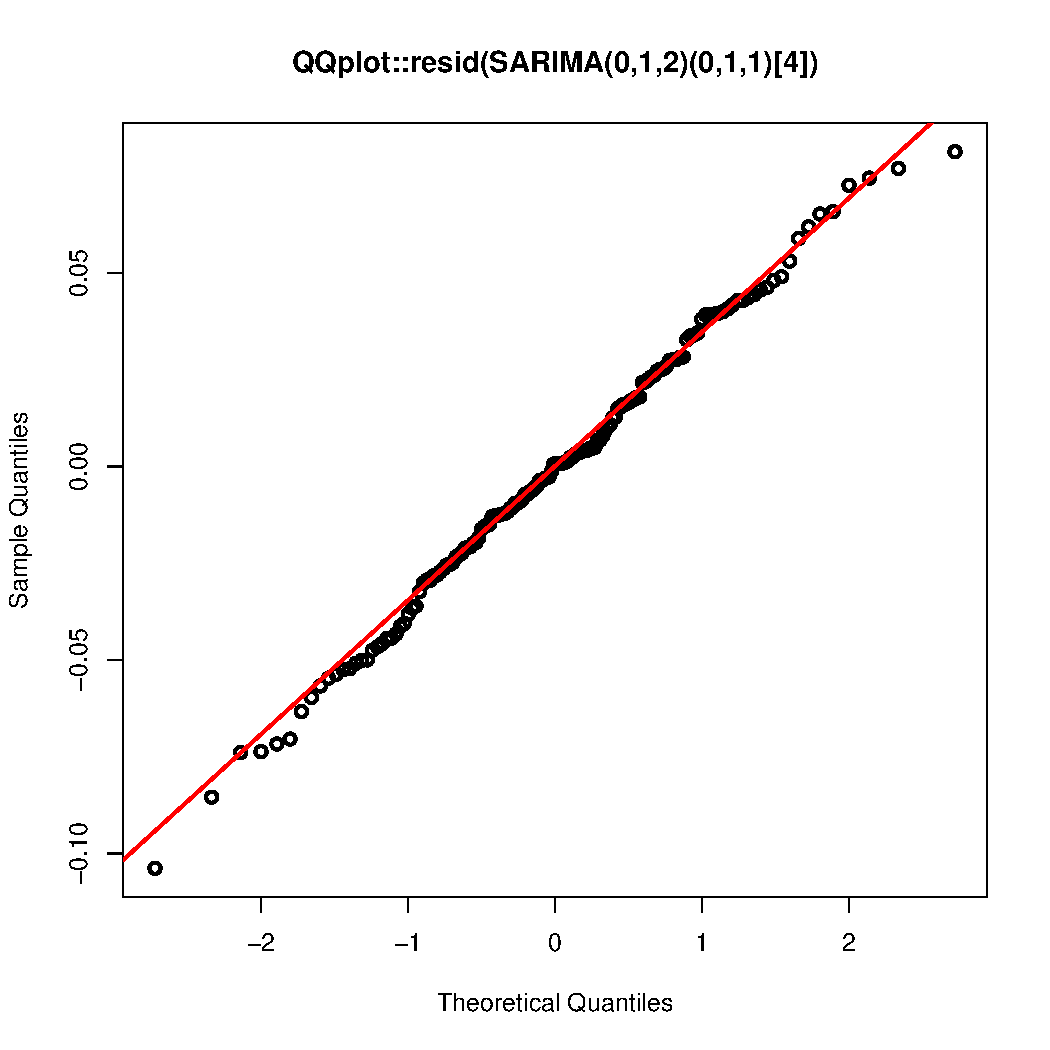
\includegraphics[width=\maxwidth]{figure/unnamed-chunk-20-3} 

\end{knitrout}
The distribution of residuals can be regard as a gaussian distribution.

So, SARIMA(0,1,2)(0,1,1)[4] is a good model.
\bigskip
4. Another method is to use Triple exponential smoothing
\begin{knitrout}
\definecolor{shadecolor}{rgb}{0.969, 0.969, 0.969}\color{fgcolor}\begin{kframe}
\begin{alltt}
\hlstd{DES_fit} \hlkwb{<-} \hlkwd{hw}\hlstd{(beer,} \hlkwc{initial} \hlstd{=} \hlstr{"optimal"}\hlstd{,} \hlkwc{seasonal} \hlstd{=} \hlstr{"additive"}\hlstd{,} \hlkwc{h} \hlstd{=} \hlnum{6}\hlstd{)}
\hlstd{DES_fit}
\end{alltt}
\begin{verbatim}
##         Point Forecast    Lo 80    Hi 80    Lo 95    Hi 95
## 1994 Q3       394.5326 373.2603 415.8050 361.9994 427.0659
## 1994 Q4       514.1839 491.8614 536.5065 480.0445 548.3234
## 1995 Q1       419.3392 395.7355 442.9429 383.2404 455.4379
## 1995 Q2       376.3166 349.5231 403.1101 335.3394 417.2937
## 1995 Q3       381.2753 352.8547 409.6960 337.8097 424.7410
## 1995 Q4       500.9267 470.6690 531.1844 454.6515 547.2018
\end{verbatim}
\begin{alltt}
\hlkwd{plot}\hlstd{(DES_fit,}\hlkwc{main} \hlstd{=} \hlstr{"Beer Forecasts from triple Exponential Smoothing"}\hlstd{,} \hlkwc{lwd} \hlstd{=} \hlnum{2}\hlstd{)}
\end{alltt}
\end{kframe}
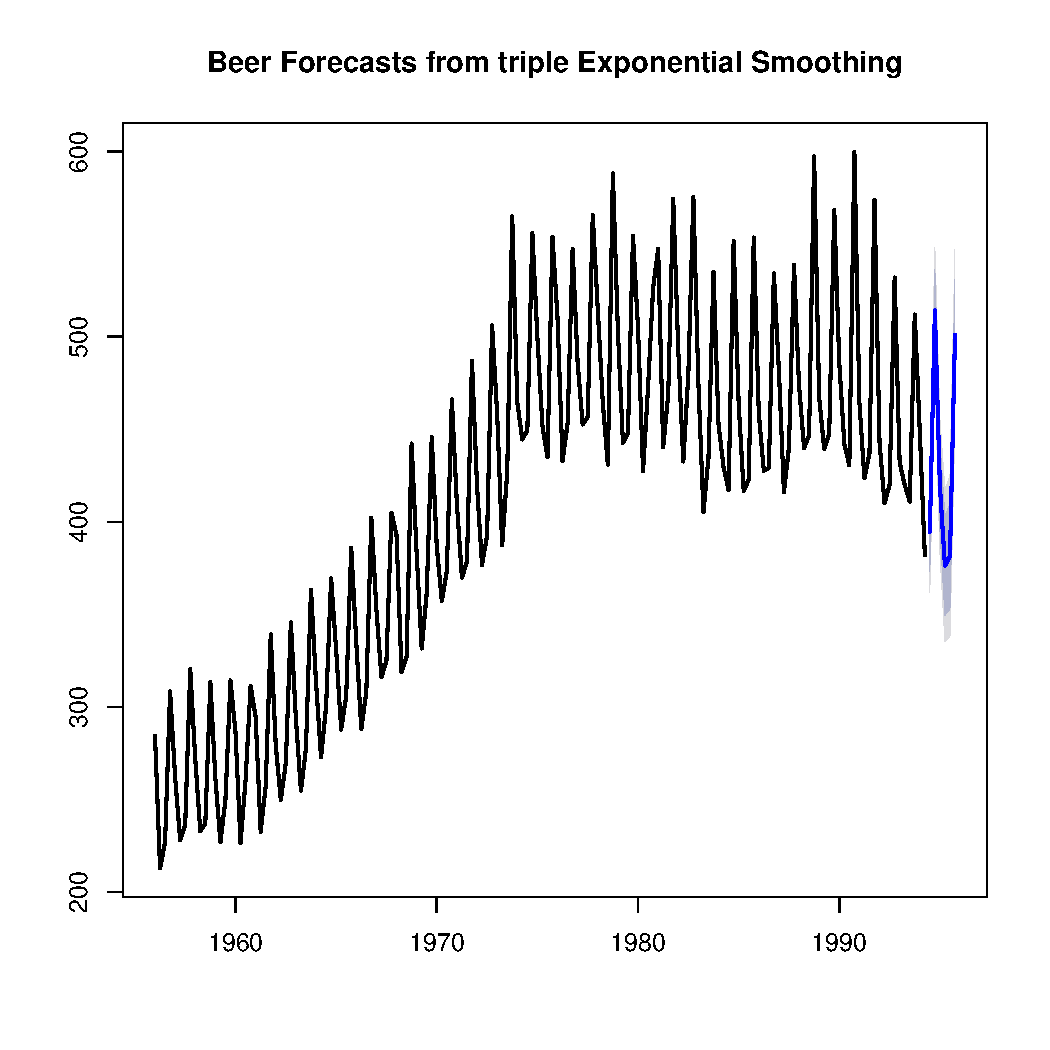
\includegraphics[width=\maxwidth]{figure/unnamed-chunk-21-1} 

\end{knitrout}

5. Use cross-validation to compare these two models

\begin{knitrout}
\definecolor{shadecolor}{rgb}{0.969, 0.969, 0.969}\color{fgcolor}\begin{kframe}
\begin{alltt}
\hlstd{CV} \hlkwb{<-}  \hlkwa{function}\hlstd{(}\hlkwc{time_series}\hlstd{,} \hlkwc{start}\hlstd{,} \hlkwc{forecast_length}\hlstd{,}\hlkwc{ts_model}\hlstd{)\{}
  \hlstd{ts_length} \hlkwb{<-}  \hlkwd{length}\hlstd{(time_series)}
  \hlstd{accuracy_list} \hlkwb{=} \hlkwd{c}\hlstd{()}
  \hlkwa{for}\hlstd{(k} \hlkwa{in} \hlstd{start}\hlopt{:}\hlstd{(ts_length} \hlopt{-} \hlstd{forecast_length))\{}
    \hlstd{fitted_model} \hlkwb{<-} \hlkwd{ts_model}\hlstd{(}\hlkwd{ts}\hlstd{(time_series[}\hlnum{0}\hlopt{:}\hlstd{k],}\hlkwc{frequency} \hlstd{=} \hlnum{4}\hlstd{))}
    \hlstd{RMSE} \hlkwb{<-}  \hlkwd{accuracy}\hlstd{(}\hlkwd{forecast}\hlstd{(fitted_model,} \hlkwc{h} \hlstd{= forecast_length))[}\hlnum{2}\hlstd{]}
    \hlstd{accuracy_list} \hlkwb{=} \hlkwd{c}\hlstd{(accuracy_list, RMSE)}
  \hlstd{\}}
  \hlkwd{return}\hlstd{(accuracy_list)}
\hlstd{\}}

\hlcom{#Define two models}
\hlstd{model_SARIMA} \hlkwb{<-} \hlkwa{function}\hlstd{(}\hlkwc{ts}\hlstd{)}
  \hlkwd{return}\hlstd{(}\hlkwd{Arima}\hlstd{(ts,} \hlkwc{order} \hlstd{=} \hlkwd{c}\hlstd{(}\hlnum{0}\hlstd{,}\hlnum{1}\hlstd{,}\hlnum{2}\hlstd{),} \hlkwc{seasonal} \hlstd{=} \hlkwd{c}\hlstd{(}\hlnum{0}\hlstd{,}\hlnum{1}\hlstd{,}\hlnum{1}\hlstd{)))}
\hlstd{model_TES} \hlkwb{<-} \hlkwa{function}\hlstd{(}\hlkwc{ts}\hlstd{)}
  \hlkwd{return}\hlstd{(}\hlkwd{hw}\hlstd{(ts,}\hlkwc{initial} \hlstd{=} \hlstr{"optimal"}\hlstd{,} \hlkwc{seasonal} \hlstd{=} \hlstr{"additive"}\hlstd{))}

\hlstd{start} \hlkwb{<-} \hlnum{90}
\hlstd{forecast_length} \hlkwb{<-} \hlnum{6}
\hlstd{CV_beer} \hlkwb{<-} \hlkwd{data.frame}\hlstd{(}
  \hlkwc{sarima} \hlstd{=} \hlkwd{CV}\hlstd{(log_beer, start, forecast_length, model_SARIMA),}
  \hlkwc{tes} \hlstd{=} \hlkwd{CV}\hlstd{(log_beer, start, forecast_length, model_TES)}
\hlstd{)}

\hlkwd{boxplot}\hlstd{(CV_beer,}\hlkwc{main} \hlstd{=} \hlstr{"Beer::Cross Validation for RMSE"}\hlstd{,} \hlkwc{lwd}\hlstd{=}\hlnum{2}\hlstd{)}
\end{alltt}
\end{kframe}
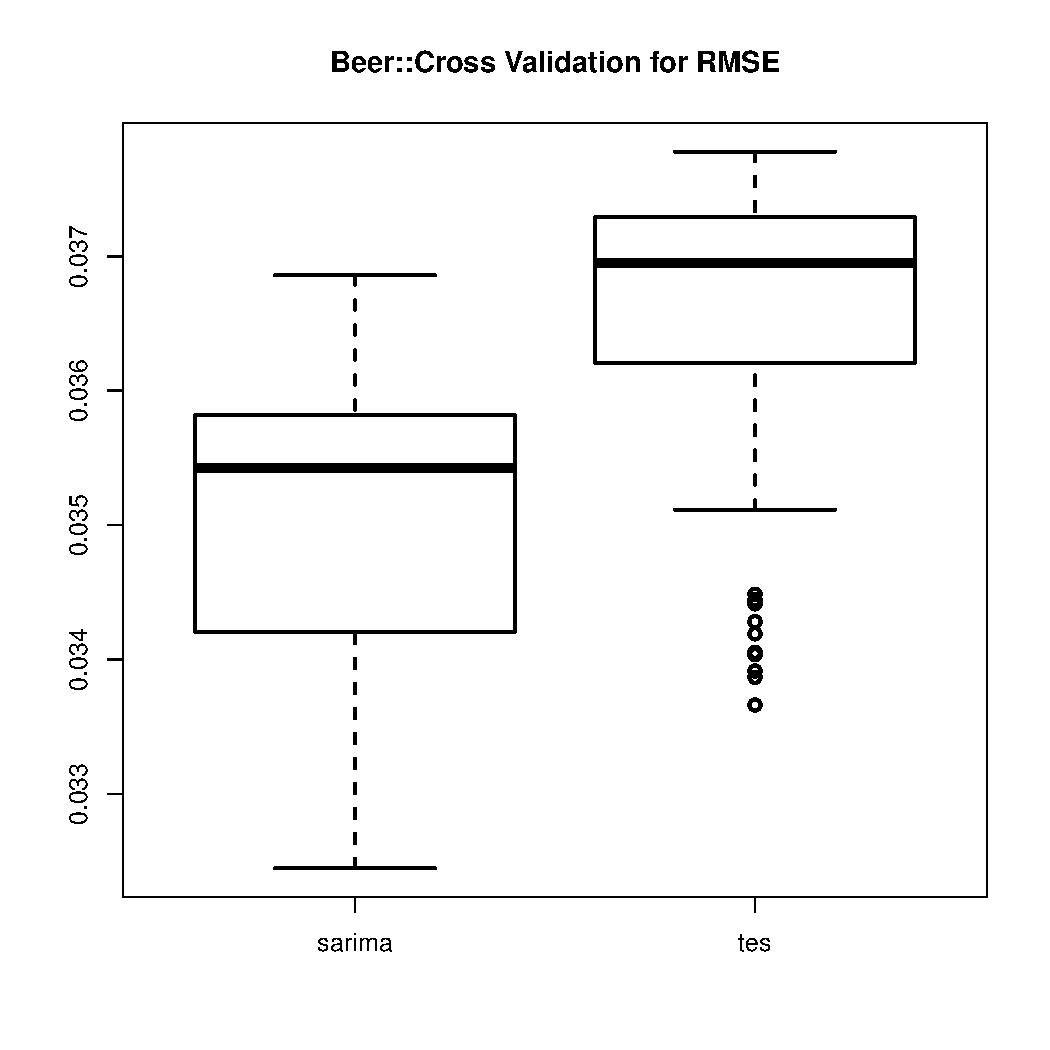
\includegraphics[width=\maxwidth]{figure/unnamed-chunk-22-1} 

\end{knitrout}

From boxplot, SARIMA(0,1,2)(0,1,1)[4] gives a better prediction, because it gives a lower RMSE.
\bigskip
6. Forecast the number of birth during the two weeks by using SARIMA(0,1,2)(0,1,1)[4].

\begin{knitrout}
\definecolor{shadecolor}{rgb}{0.969, 0.969, 0.969}\color{fgcolor}\begin{kframe}
\begin{alltt}
\hlstd{sarima_forecast} \hlkwb{<-} \hlkwd{forecast}\hlstd{(sarima_fit,} \hlkwc{h} \hlstd{=} \hlnum{6}\hlstd{)}
\hlstd{sarima_forecast}\hlopt{$}\hlstd{x}\hlkwb{<-}\hlkwd{exp}\hlstd{(sarima_forecast}\hlopt{$}\hlstd{x)}
\hlstd{sarima_forecast}\hlopt{$}\hlstd{lower}\hlkwb{<-}\hlkwd{exp}\hlstd{(sarima_forecast}\hlopt{$}\hlstd{lower)}
\hlstd{sarima_forecast}\hlopt{$}\hlstd{upper}\hlkwb{<-}\hlkwd{exp}\hlstd{(sarima_forecast}\hlopt{$}\hlstd{upper)}
\hlstd{sarima_forecast}\hlopt{$}\hlstd{mean}\hlkwb{<-}\hlkwd{exp}\hlstd{(sarima_forecast}\hlopt{$}\hlstd{mean)}
\hlstd{sarima_forecast}
\end{alltt}
\begin{verbatim}
##         Point Forecast    Lo 80    Hi 80    Lo 95    Hi 95
## 1994 Q3       407.0242 388.5254 426.4037 379.0755 437.0334
## 1994 Q4       512.2461 488.9607 536.6404 477.0658 550.0208
## 1995 Q1       425.5336 404.5116 447.6481 393.8069 459.8163
## 1995 Q2       386.4387 365.9450 408.0801 355.5399 420.0228
## 1995 Q3       395.0946 371.2026 420.5244 359.1455 434.6421
## 1995 Q4       504.3541 472.3371 538.5413 456.2195 557.5673
\end{verbatim}
\begin{alltt}
\hlkwd{plot}\hlstd{(sarima_forecast,} \hlkwc{main} \hlstd{=} \hlstr{"Beer Forecasts from SARIMA(0,1,2)(0,1,1)[4]"}\hlstd{,}\hlkwc{lwd} \hlstd{=} \hlnum{2}\hlstd{)}
\end{alltt}
\end{kframe}
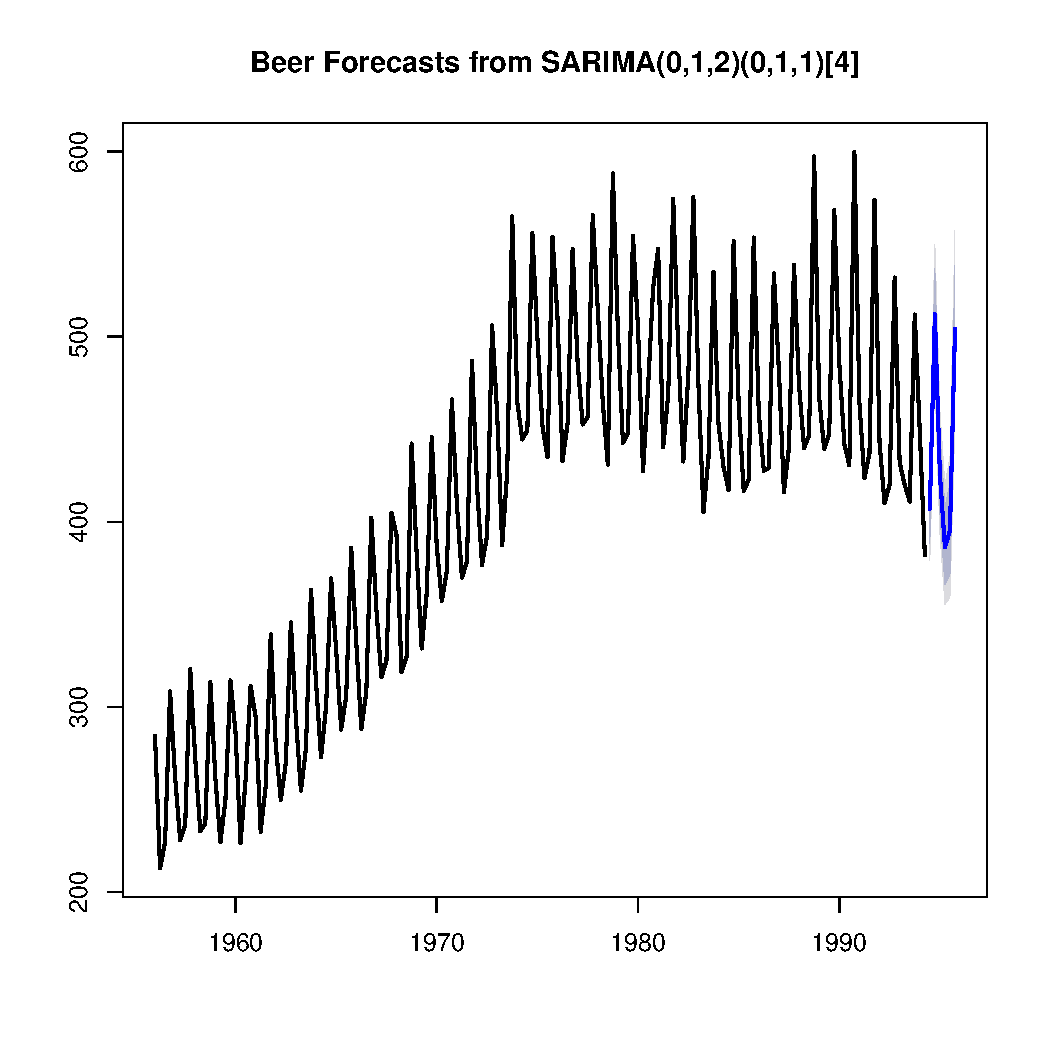
\includegraphics[width=\maxwidth]{figure/unnamed-chunk-23-1} 

\end{knitrout}


\section{ Exercise 4 (Temperature in Singapore?)}

1. Load the data and plot.
\begin{knitrout}
\definecolor{shadecolor}{rgb}{0.969, 0.969, 0.969}\color{fgcolor}\begin{kframe}
\begin{alltt}
\hlstd{temp_data} \hlkwb{<-} \hlkwd{read.csv}\hlstd{(}\hlstr{"E:/ST3233/Assignment2/Datasets/temperature_in_singapore.csv"}\hlstd{,}
                      \hlkwc{header}\hlstd{=} \hlnum{TRUE}\hlstd{,}\hlkwc{sep}\hlstd{=}\hlstr{","}\hlstd{)}
\hlstd{temp} \hlkwb{<-} \hlkwd{ts}\hlstd{(temp_data}\hlopt{$}\hlstd{mean_temp,}\hlkwc{frequency} \hlstd{=} \hlnum{12}\hlstd{,}
           \hlkwc{start}\hlstd{=}\hlkwd{c}\hlstd{(}\hlnum{1982}\hlstd{,}\hlnum{1}\hlstd{))}
\hlkwd{par}\hlstd{(}\hlkwc{mfrow}\hlstd{=}\hlkwd{c}\hlstd{(}\hlnum{1}\hlstd{,}\hlnum{1}\hlstd{))}
\hlkwd{plot}\hlstd{(temp,}\hlkwc{lwd} \hlstd{=} \hlnum{2}\hlstd{,} \hlkwc{main} \hlstd{=} \hlstr{"Temperature in SG"}\hlstd{)}
\end{alltt}
\end{kframe}
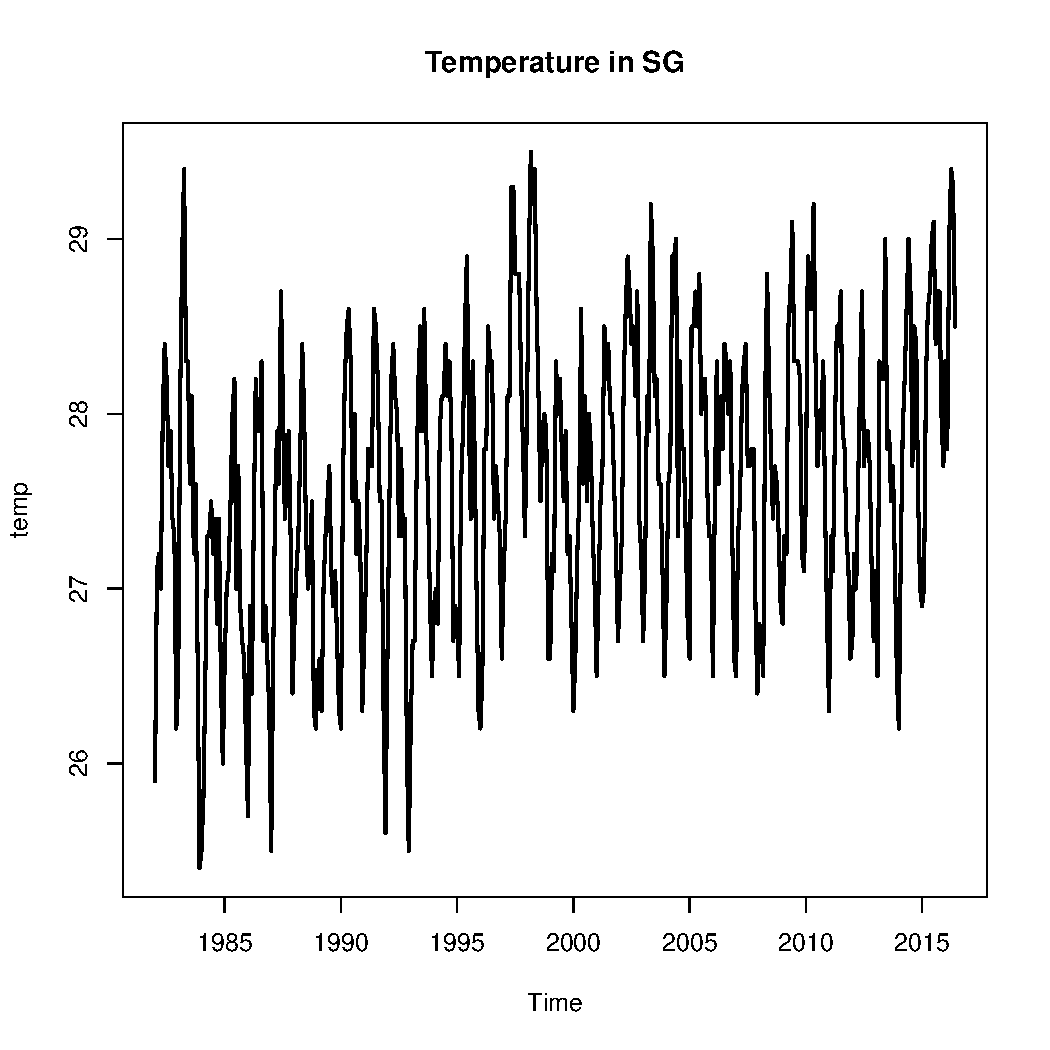
\includegraphics[width=\maxwidth]{figure/unnamed-chunk-24-1} 
\begin{kframe}\begin{alltt}
\hlkwd{acf}\hlstd{(temp,}\hlkwc{lwd} \hlstd{=} \hlnum{2} \hlstd{,} \hlkwc{main} \hlstd{=} \hlstr{"ACF::Temp"}\hlstd{)}
\end{alltt}
\end{kframe}
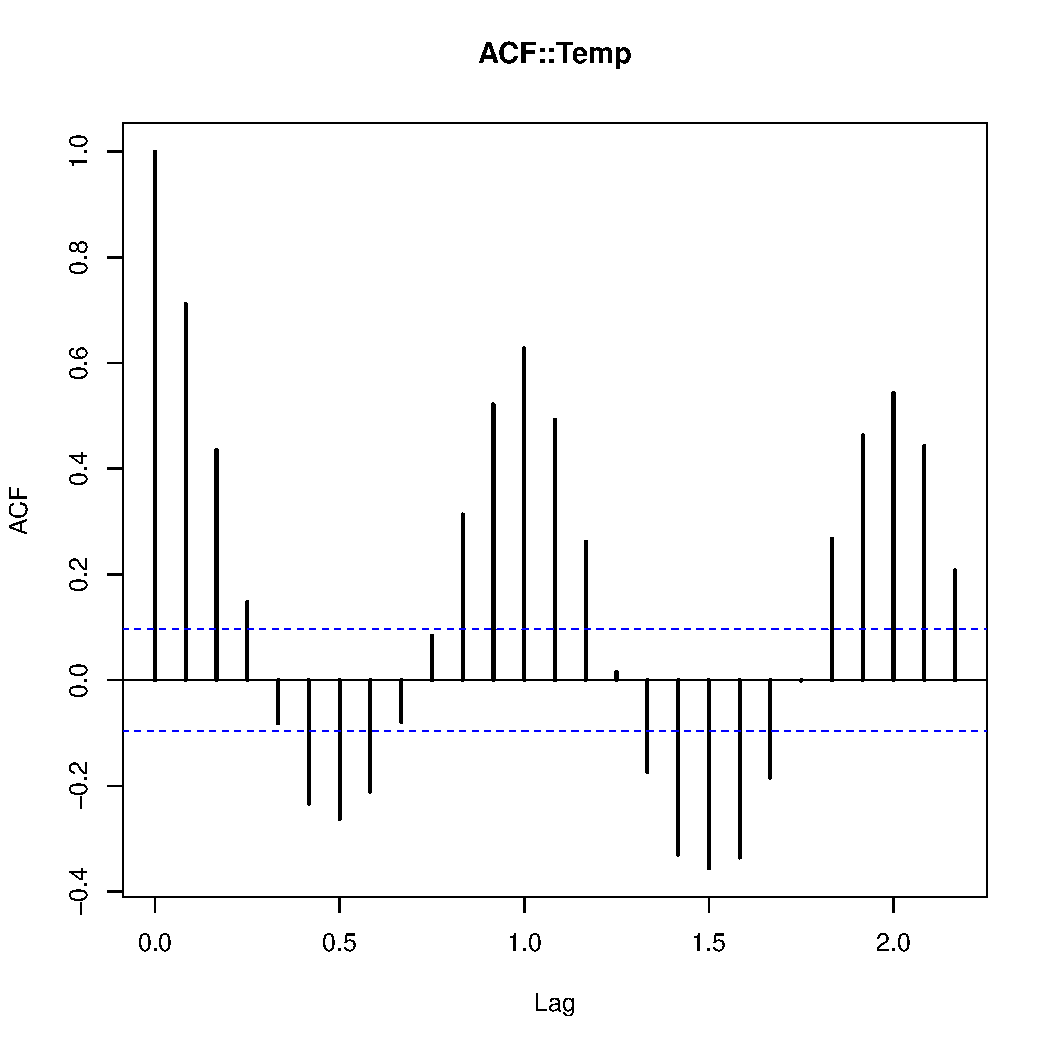
\includegraphics[width=\maxwidth]{figure/unnamed-chunk-24-2} 
\begin{kframe}\begin{alltt}
\hlcom{#The time series \{temp\} is not stationary and has seasonal behavior, decompose it.}
\hlstd{temp_decmp} \hlkwb{<-}\hlkwd{stl}\hlstd{(temp,}\hlkwc{s.window} \hlstd{=} \hlstr{"periodic"}\hlstd{,} \hlkwc{robust} \hlstd{= T)}
\hlkwd{plot}\hlstd{(temp_decmp)}
\end{alltt}
\end{kframe}
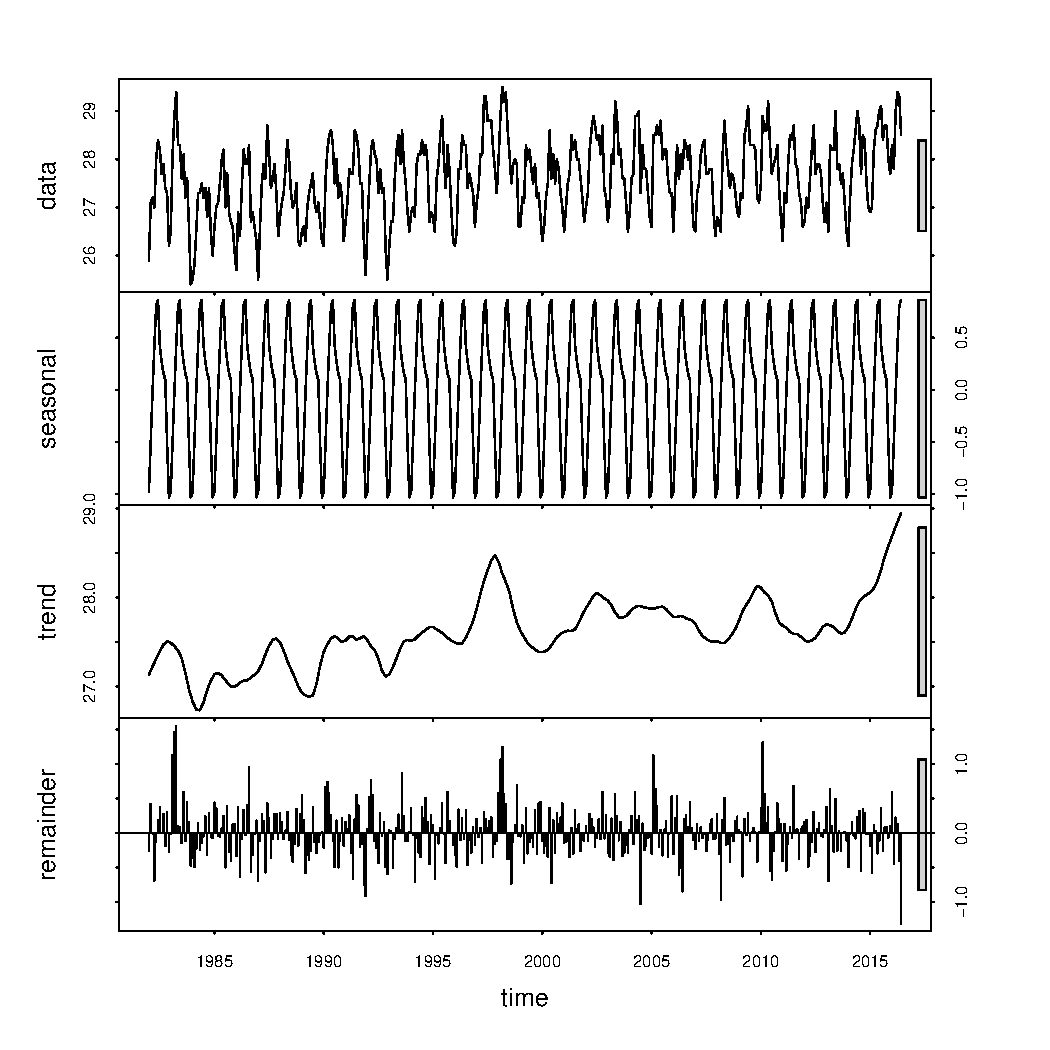
\includegraphics[width=\maxwidth]{figure/unnamed-chunk-24-3} 
\begin{kframe}\begin{alltt}
\hlkwd{seasonplot}\hlstd{(temp}\hlopt{-}\hlstd{temp_decmp}\hlopt{$}\hlstd{time.series[,}\hlstr{"trend"}\hlstd{],}\hlkwc{s} \hlstd{=} \hlnum{12}\hlstd{,} \hlkwc{col} \hlstd{=} \hlnum{1}\hlopt{:}\hlnum{12}\hlstd{,} \hlkwc{type} \hlstd{=} \hlstr{"l"}\hlstd{)}
\end{alltt}
\end{kframe}
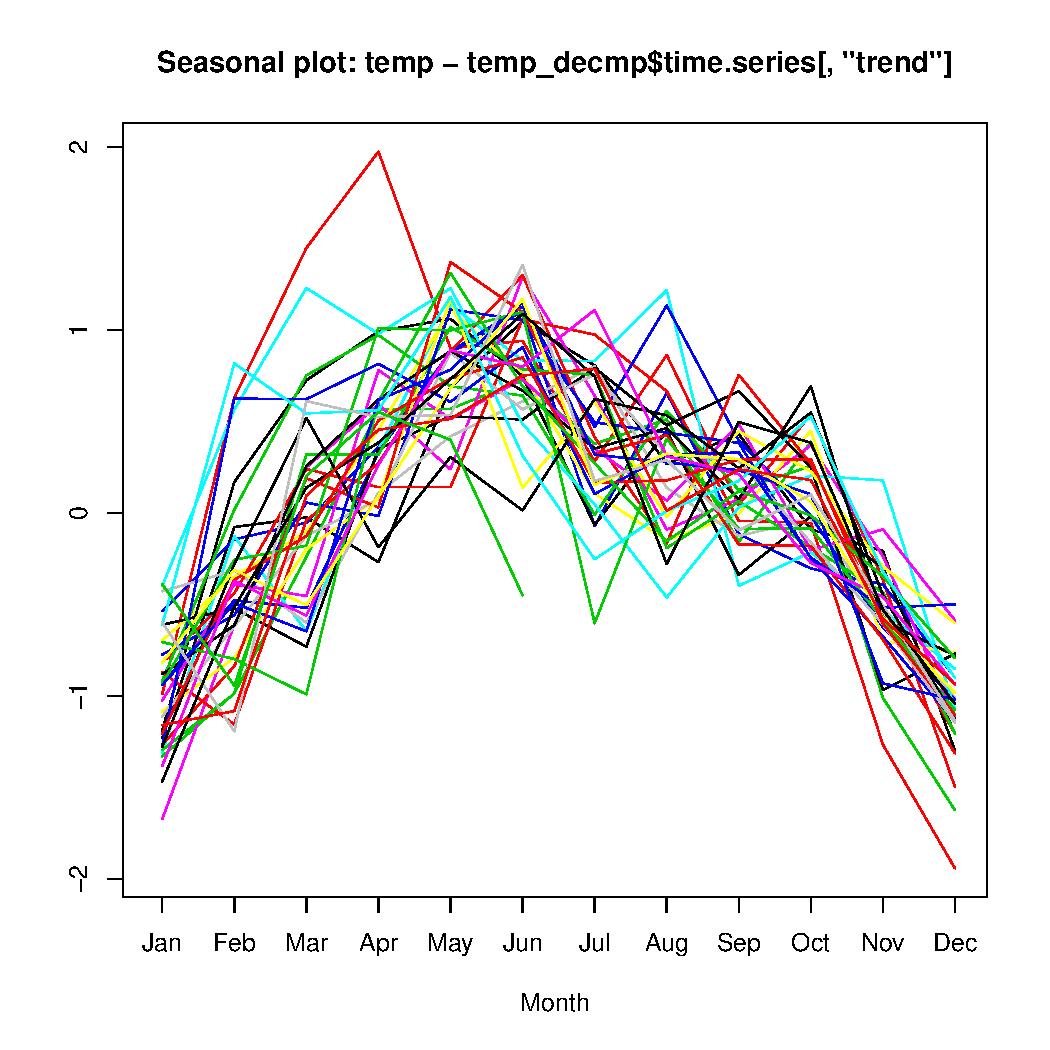
\includegraphics[width=\maxwidth]{figure/unnamed-chunk-24-4} 

\end{knitrout}
There is seasonal component and trend, thus, use SARIMA model
\bigskip
2. Fit the SARIMA model.

\begin{knitrout}
\definecolor{shadecolor}{rgb}{0.969, 0.969, 0.969}\color{fgcolor}\begin{kframe}
\begin{alltt}
\hlstd{temp_d12} \hlkwb{=} \hlkwd{diff}\hlstd{(temp,} \hlkwc{lag} \hlstd{=} \hlnum{12}\hlstd{)}
\hlkwd{plot}\hlstd{(temp_d12,}\hlkwc{lwd} \hlstd{=} \hlnum{2}\hlstd{,} \hlkwc{main} \hlstd{=} \hlstr{"diff(temp, lag = 12)"}\hlstd{)}
\end{alltt}
\end{kframe}
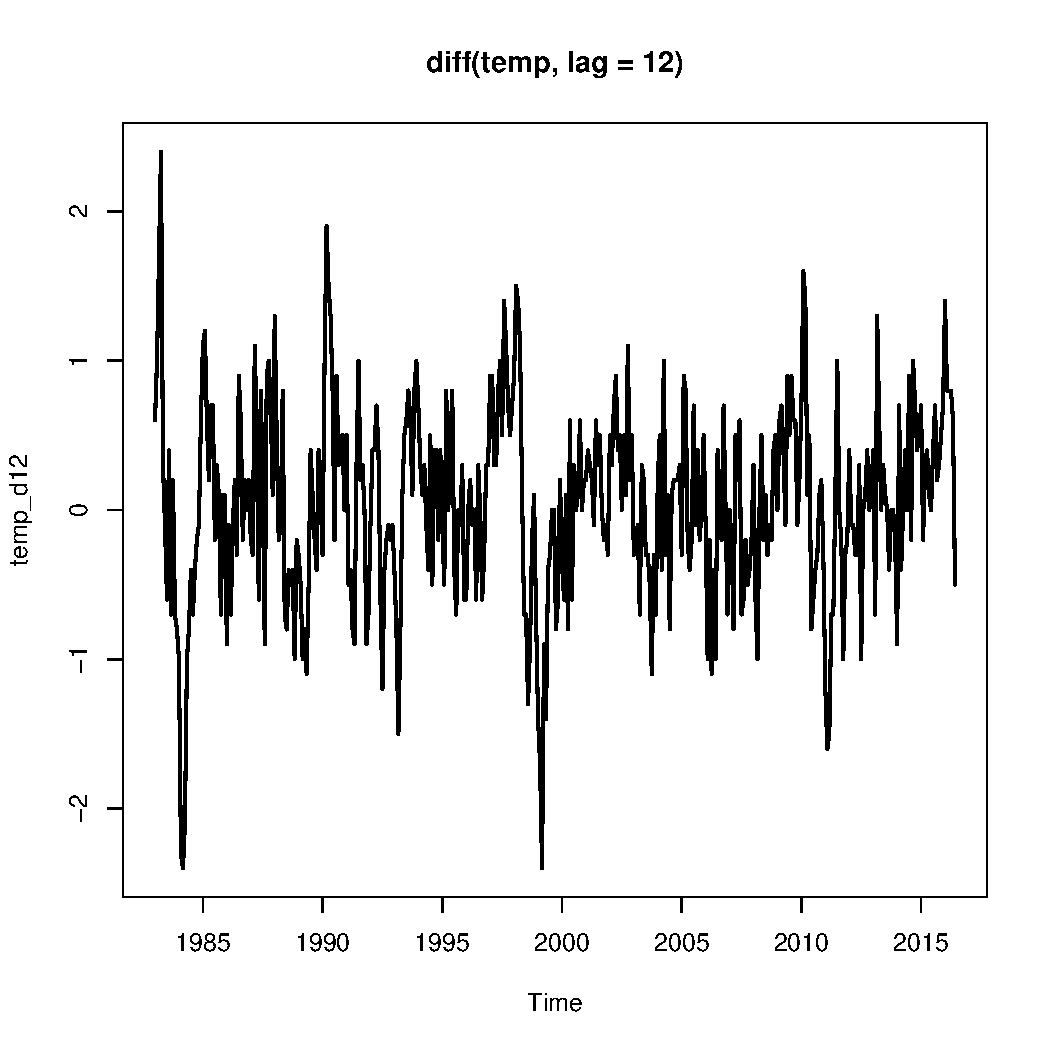
\includegraphics[width=\maxwidth]{figure/unnamed-chunk-25-1} 
\begin{kframe}\begin{alltt}
\hlstd{temp_d12_d1} \hlkwb{=} \hlkwd{diff}\hlstd{(temp_d12,} \hlkwc{lag} \hlstd{=} \hlnum{1}\hlstd{)}
\hlkwd{plot}\hlstd{(temp_d12_d1,}\hlkwc{lwd} \hlstd{=} \hlnum{2}\hlstd{,} \hlkwc{main} \hlstd{=} \hlstr{"diff(diff(temp, lag = 12))"}\hlstd{)}
\end{alltt}
\end{kframe}
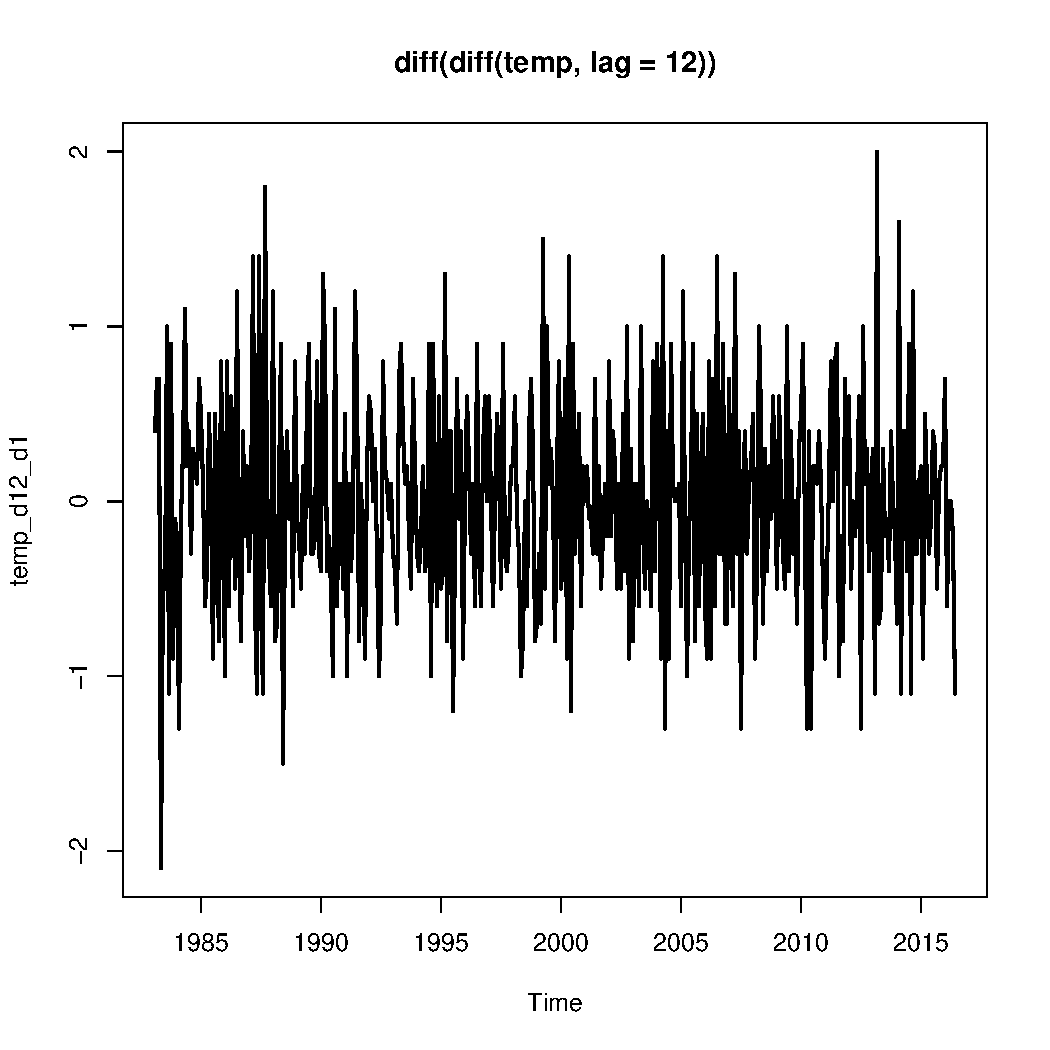
\includegraphics[width=\maxwidth]{figure/unnamed-chunk-25-2} 
\begin{kframe}\begin{alltt}
\hlkwd{par}\hlstd{(}\hlkwc{mfrow}\hlstd{=}\hlkwd{c}\hlstd{(}\hlnum{2}\hlstd{,}\hlnum{1}\hlstd{))}
\hlkwd{acf}\hlstd{(temp_d12_d1,}\hlkwc{lwd} \hlstd{=} \hlnum{2}\hlstd{,} \hlkwc{main} \hlstd{=} \hlstr{"ACF::diff(diff(temp, lag = 12))"}\hlstd{)}
\hlkwd{pacf}\hlstd{(temp_d12_d1,}\hlkwc{lwd} \hlstd{=} \hlnum{2}\hlstd{,} \hlkwc{main} \hlstd{=} \hlstr{"PACF::diff(diff(temp, lag = 12))"}\hlstd{)}
\end{alltt}
\end{kframe}
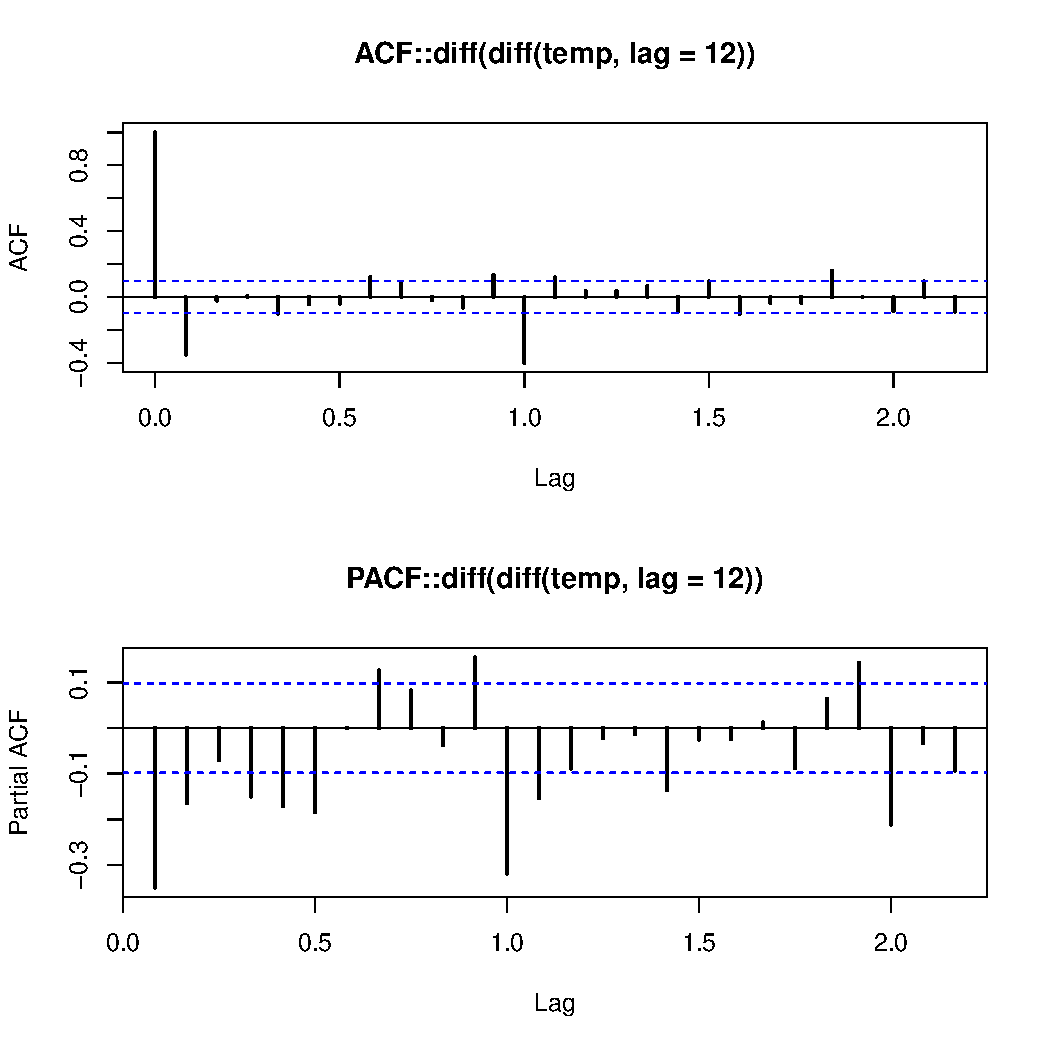
\includegraphics[width=\maxwidth]{figure/unnamed-chunk-25-3} 

\end{knitrout}
From acf plot ,q \leq 1, and from partial-acf plot, p \leq 5 with d = D = 1 and P \leq 1, Q \leq 1.

\begin{knitrout}
\definecolor{shadecolor}{rgb}{0.969, 0.969, 0.969}\color{fgcolor}\begin{kframe}
\begin{alltt}
\hlstd{AIC_best} \hlkwb{<-} \hlnum{10}\hlopt{**}\hlnum{6}
\hlkwa{for} \hlstd{(p} \hlkwa{in} \hlnum{0}\hlopt{:}\hlnum{5}\hlstd{)\{}
  \hlkwa{for} \hlstd{(q} \hlkwa{in} \hlnum{0}\hlopt{:}\hlnum{1}\hlstd{)\{}
    \hlkwa{for} \hlstd{(P} \hlkwa{in} \hlnum{0}\hlopt{:}\hlnum{1}\hlstd{)\{}
      \hlkwa{for} \hlstd{(Q} \hlkwa{in} \hlnum{0}\hlopt{:}\hlnum{1}\hlstd{)\{}
        \hlstd{fit_sarima} \hlkwb{<-} \hlkwd{Arima}\hlstd{(temp,} \hlkwc{order} \hlstd{=} \hlkwd{c}\hlstd{(p,}\hlnum{1}\hlstd{,q),}\hlkwc{seasonal} \hlstd{=} \hlkwd{c}\hlstd{(P,}\hlnum{1}\hlstd{,Q))}
        \hlkwa{if} \hlstd{(fit_sarima}\hlopt{$}\hlstd{aic} \hlopt{<} \hlstd{AIC_best)\{}
          \hlstd{AIC_best} \hlkwb{<-} \hlstd{fit_sarima}\hlopt{$}\hlstd{aic}
          \hlkwd{cat}\hlstd{(}\hlstr{"p = "}\hlstd{,p,}\hlstr{", q = "}\hlstd{,q,}\hlstr{",P = "}\hlstd{,P,}\hlstr{",Q = "}\hlstd{,Q,}\hlstr{"\textbackslash{}t AIC = "}\hlstd{,AIC_best,}\hlstr{"\textbackslash{}n"}\hlstd{)}
        \hlstd{\}}
      \hlstd{\}}
    \hlstd{\}}
  \hlstd{\}}
\hlstd{\}}
\end{alltt}
\begin{verbatim}
## p =  0 , q =  0 ,P =  0 ,Q =  0 	 AIC =  780.5999 
## p =  0 , q =  0 ,P =  0 ,Q =  1 	 AIC =  596.2691 
## p =  0 , q =  0 ,P =  1 ,Q =  1 	 AIC =  593.1758 
## p =  0 , q =  1 ,P =  0 ,Q =  1 	 AIC =  493.1153 
## p =  1 , q =  1 ,P =  0 ,Q =  1 	 AIC =  488.5129 
## p =  2 , q =  1 ,P =  0 ,Q =  1 	 AIC =  483.6007 
## p =  2 , q =  1 ,P =  1 ,Q =  1 	 AIC =  483.2574 
## p =  3 , q =  1 ,P =  0 ,Q =  1 	 AIC =  483.1996 
## p =  3 , q =  1 ,P =  1 ,Q =  1 	 AIC =  483.1188
\end{verbatim}
\end{kframe}
\end{knitrout}

From the results, SARIMA(2,1,1)(0,1,1)[12] gives a lower AIC, with number of parameters = 4

\begin{knitrout}
\definecolor{shadecolor}{rgb}{0.969, 0.969, 0.969}\color{fgcolor}\begin{kframe}
\begin{alltt}
\hlstd{temp_fit} \hlkwb{<-} \hlkwd{Arima}\hlstd{(temp,} \hlkwc{order} \hlstd{=} \hlkwd{c}\hlstd{(}\hlnum{2}\hlstd{,}\hlnum{1}\hlstd{,}\hlnum{1}\hlstd{),} \hlkwc{seasonal} \hlstd{=} \hlkwd{c}\hlstd{(}\hlnum{0}\hlstd{,}\hlnum{1}\hlstd{,}\hlnum{1}\hlstd{))}
\end{alltt}
\end{kframe}
\end{knitrout}

3. Then consider the residuals of the SARIMA model.
\begin{knitrout}
\definecolor{shadecolor}{rgb}{0.969, 0.969, 0.969}\color{fgcolor}\begin{kframe}
\begin{alltt}
\hlkwd{par}\hlstd{(}\hlkwc{mfrow}\hlstd{=}\hlkwd{c}\hlstd{(}\hlnum{1}\hlstd{,}\hlnum{1}\hlstd{))}
\hlkwd{plot}\hlstd{(}\hlkwd{resid}\hlstd{(temp_fit),}\hlkwc{lwd}\hlstd{=}\hlnum{2}\hlstd{,} \hlkwc{main}\hlstd{=}\hlstr{"resid(SARIMA(2,1,1)(0,1,1)[12])"}\hlstd{)}
\end{alltt}
\end{kframe}
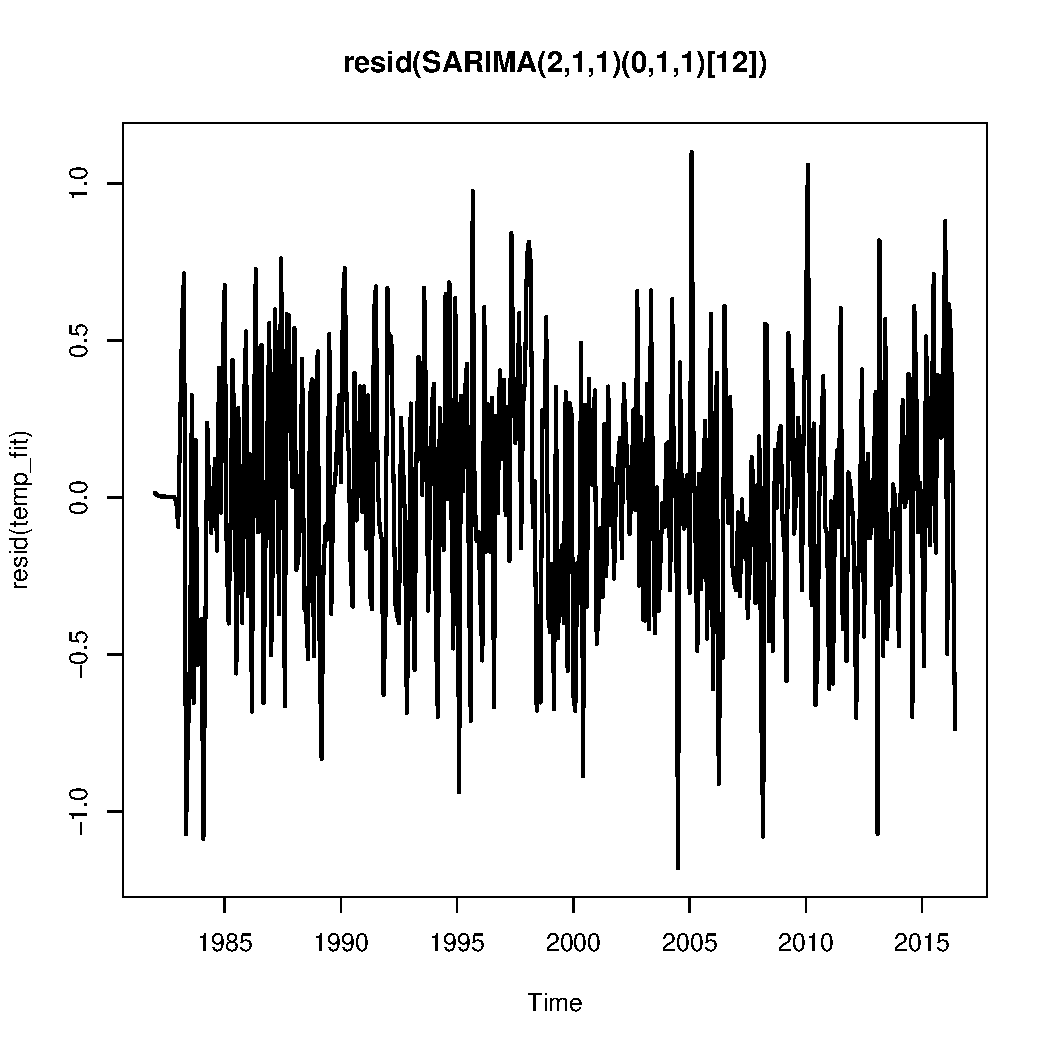
\includegraphics[width=\maxwidth]{figure/unnamed-chunk-28-1} 
\begin{kframe}\begin{alltt}
\hlkwd{par}\hlstd{(}\hlkwc{mfrow}\hlstd{=}\hlkwd{c}\hlstd{(}\hlnum{2}\hlstd{,}\hlnum{1}\hlstd{))}
\hlkwd{acf}\hlstd{(}\hlkwd{resid}\hlstd{(temp_fit),}\hlkwc{lwd}\hlstd{=}\hlnum{2}\hlstd{,} \hlkwc{main}\hlstd{=}\hlstr{"ACF::resid(SARIMA(2,1,1)(0,1,1)[12])"}\hlstd{,}\hlkwc{lag.max} \hlstd{=} \hlnum{11}\hlstd{)}
\hlkwd{pacf}\hlstd{(}\hlkwd{resid}\hlstd{(temp_fit),}\hlkwc{lwd}\hlstd{=}\hlnum{2}\hlstd{,} \hlkwc{main}\hlstd{=}\hlstr{"PACF::resid(SARIMA(2,1,1)(0,1,1)[12])"}\hlstd{,}\hlkwc{lag.max} \hlstd{=} \hlnum{11}\hlstd{)}
\end{alltt}
\end{kframe}
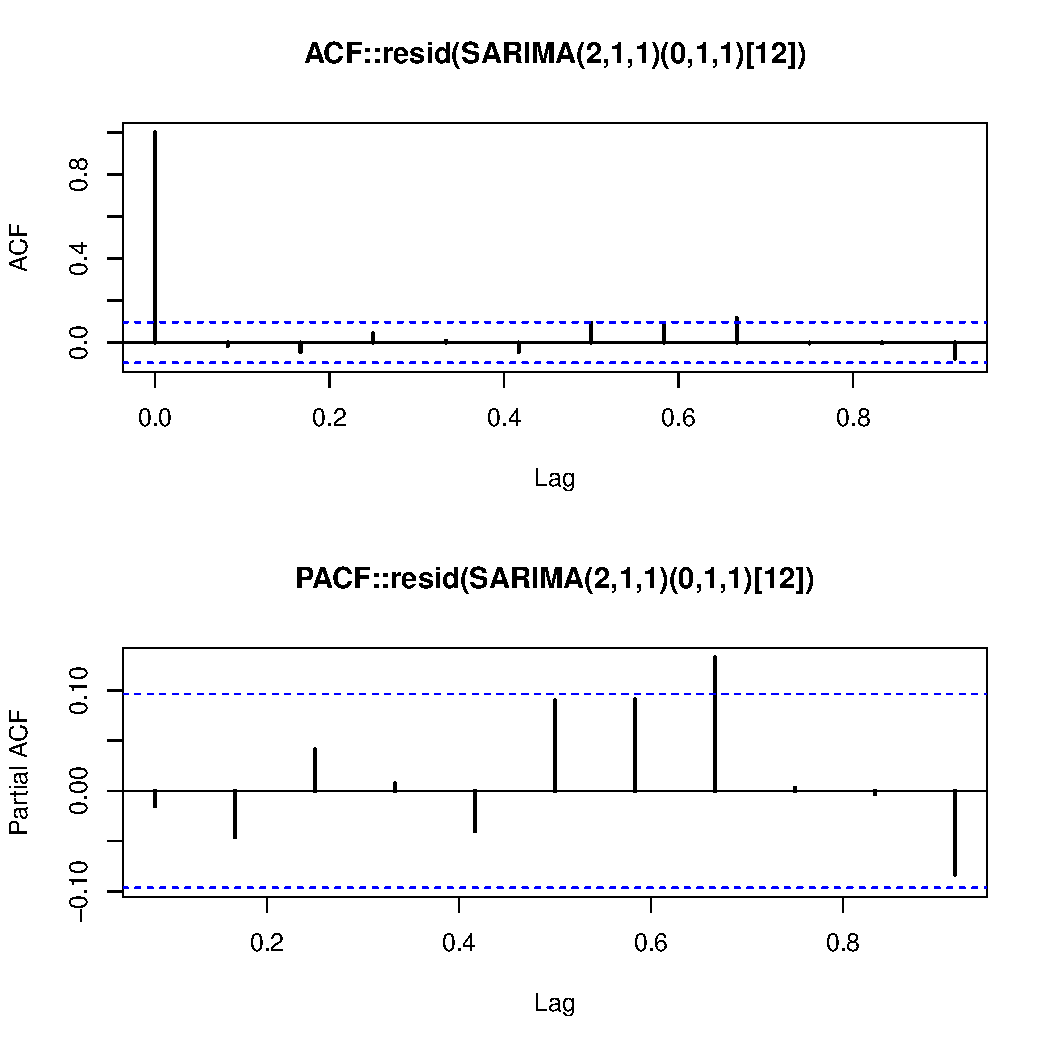
\includegraphics[width=\maxwidth]{figure/unnamed-chunk-28-2} 
\begin{kframe}\begin{alltt}
\hlcom{#The residual is stationary.}
\hlkwd{par}\hlstd{(}\hlkwc{mfrow}\hlstd{=}\hlkwd{c}\hlstd{(}\hlnum{1}\hlstd{,}\hlnum{1}\hlstd{))}
\hlkwd{qqnorm}\hlstd{(}\hlkwd{resid}\hlstd{(temp_fit),}\hlkwc{lwd}\hlstd{=}\hlnum{2}\hlstd{,} \hlkwc{main}\hlstd{=}\hlstr{"QQplot::resid(SARIMA(2,1,1)(0,1,1)[12])"}\hlstd{)}
\hlkwd{qqline}\hlstd{(}\hlkwd{resid}\hlstd{(temp_fit),} \hlkwc{lwd}\hlstd{=}\hlnum{2}\hlstd{,} \hlkwc{col}\hlstd{=}\hlstr{"red"}\hlstd{)}
\end{alltt}
\end{kframe}
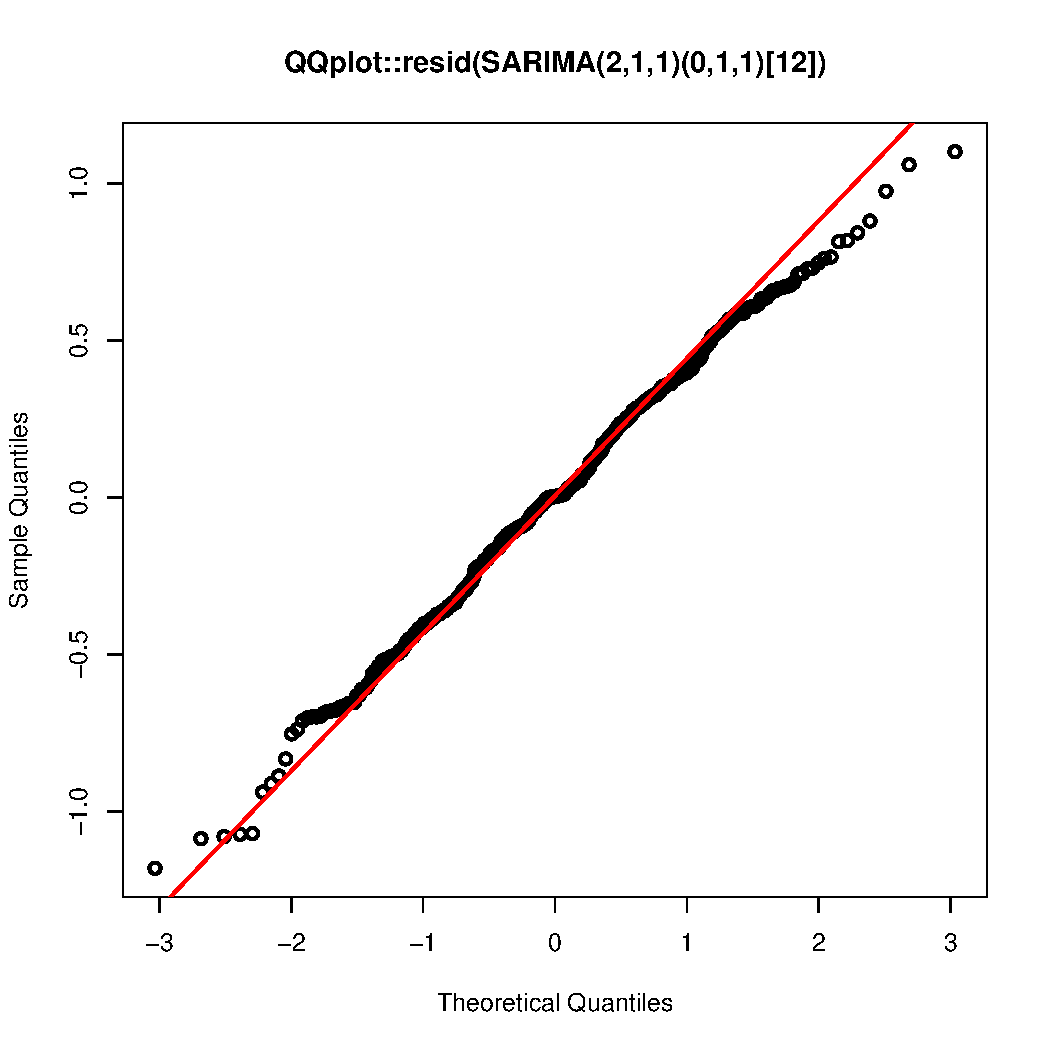
\includegraphics[width=\maxwidth]{figure/unnamed-chunk-28-3} 

\end{knitrout}
The residual follows a Gaussian Distribution.
So, SARIMA(2,1,1)(0,1,1)[12] is a good smodel.
\bigskip
4. Another method is to use Triple exponential smoothing
\begin{knitrout}
\definecolor{shadecolor}{rgb}{0.969, 0.969, 0.969}\color{fgcolor}\begin{kframe}
\begin{alltt}
\hlstd{DES_fit} \hlkwb{<-} \hlkwd{hw}\hlstd{(temp,} \hlkwc{initial} \hlstd{=} \hlstr{"optimal"}\hlstd{,} \hlkwc{seasonal} \hlstd{=} \hlstr{"additive"}\hlstd{,} \hlkwc{h} \hlstd{=} \hlnum{2}\hlopt{*}\hlnum{12}\hlstd{)}
\hlstd{DES_fit}
\end{alltt}
\begin{verbatim}
##          Point Forecast    Lo 80    Hi 80    Lo 95    Hi 95
## Jul 2016       28.73622 28.20193 29.27051 27.91910 29.55334
## Aug 2016       28.59954 28.03249 29.16659 27.73232 29.46677
## Sep 2016       28.53805 27.93993 29.13618 27.62331 29.45280
## Oct 2016       28.48181 27.85405 29.10957 27.52174 29.44188
## Nov 2016       27.81602 27.15986 28.47217 26.81252 28.81952
## Dec 2016       27.36870 26.68524 28.05216 26.32344 28.41397
## Jan 2017       27.33246 26.62266 28.04227 26.24691 28.41802
## Feb 2017       27.96003 27.22474 28.69533 26.83549 29.08457
## Mar 2017       28.39468 27.63466 29.15470 27.23234 29.55702
## Apr 2017       28.83468 28.05065 29.61872 27.63560 30.03376
## May 2017       29.20939 28.40197 30.01681 27.97455 30.44423
## Jun 2017       29.19020 28.35997 30.02044 27.92047 30.45994
## Jul 2017       28.77542 27.92291 29.62792 27.47163 30.07921
## Aug 2017       28.63874 27.76446 29.51301 27.30165 29.97582
## Sep 2017       28.57725 27.68166 29.47284 27.20757 29.94694
## Oct 2017       28.52101 27.60453 29.43749 27.11938 29.92264
## Nov 2017       27.85521 26.91824 28.79218 26.42224 29.28818
## Dec 2017       27.40790 26.45081 28.36499 25.94416 28.87164
## Jan 2018       27.37166 26.39480 28.34852 25.87768 28.86564
## Feb 2018       27.99923 27.00293 28.99554 26.47551 29.52295
## Mar 2018       28.43388 27.41844 29.44932 26.88089 29.98686
## Apr 2018       28.87388 27.83959 29.90816 27.29208 30.45568
## May 2018       29.24859 28.19574 30.30144 27.63839 30.85878
## Jun 2018       29.22940 28.15823 30.30057 27.59119 30.86761
\end{verbatim}
\begin{alltt}
\hlkwd{plot}\hlstd{(DES_fit,}\hlkwc{main} \hlstd{=} \hlstr{"Temperature Forecasts from triple Exponential Smoothing"}\hlstd{,} \hlkwc{lwd} \hlstd{=} \hlnum{2}\hlstd{)}
\end{alltt}
\end{kframe}
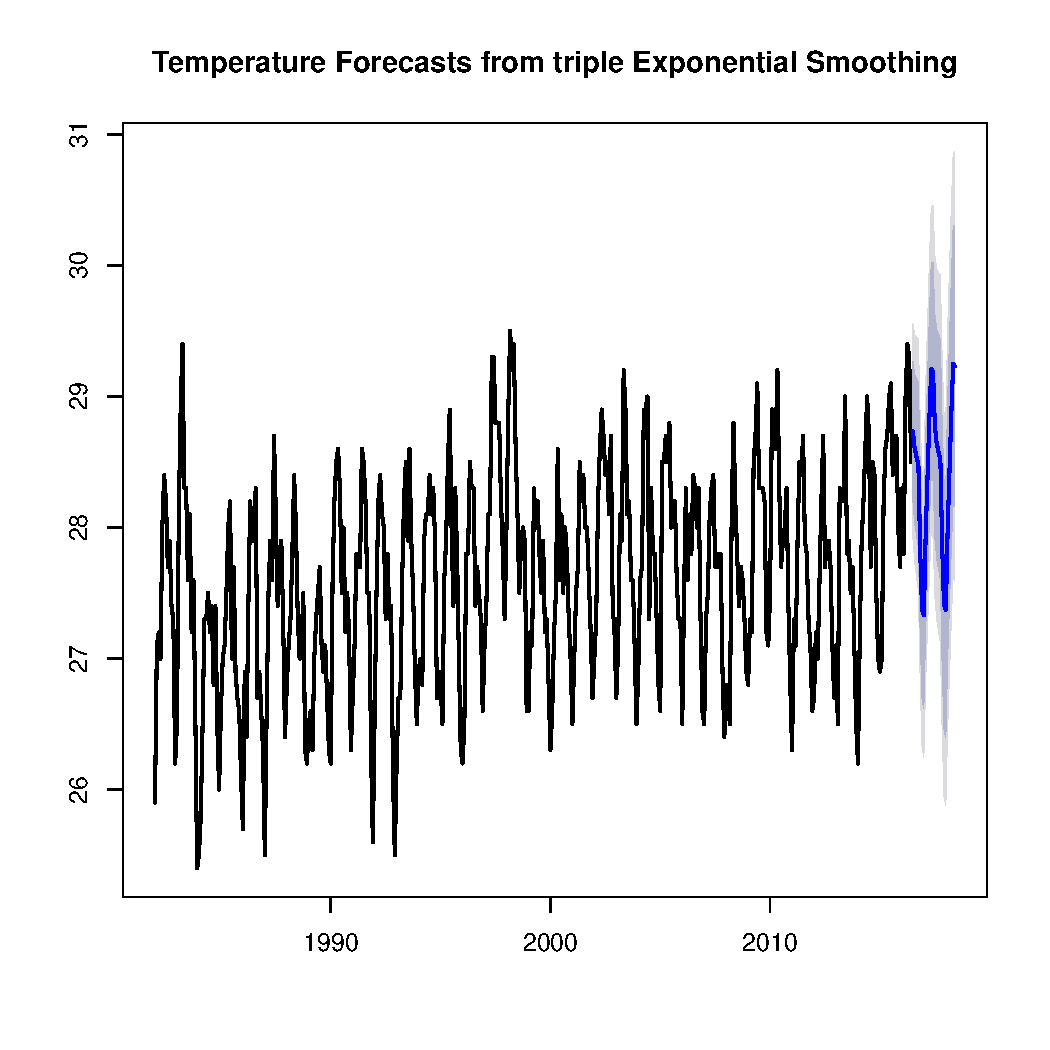
\includegraphics[width=\maxwidth]{figure/unnamed-chunk-29-1} 

\end{knitrout}

5. Use cross-validation to compare these two models
\begin{knitrout}
\definecolor{shadecolor}{rgb}{0.969, 0.969, 0.969}\color{fgcolor}\begin{kframe}
\begin{alltt}
\hlstd{CV} \hlkwb{<-}  \hlkwa{function}\hlstd{(}\hlkwc{time_series}\hlstd{,} \hlkwc{start}\hlstd{,} \hlkwc{forecast_length}\hlstd{,}\hlkwc{ts_model}\hlstd{)\{}
  \hlstd{ts_length} \hlkwb{<-}  \hlkwd{length}\hlstd{(time_series)}
  \hlstd{accuracy_list} \hlkwb{=} \hlkwd{c}\hlstd{()}
  \hlkwa{for}\hlstd{(k} \hlkwa{in} \hlstd{start}\hlopt{:}\hlstd{(ts_length} \hlopt{-} \hlstd{forecast_length))\{}
    \hlstd{fitted_model} \hlkwb{<-} \hlkwd{ts_model}\hlstd{(}\hlkwd{ts}\hlstd{(time_series[}\hlnum{0}\hlopt{:}\hlstd{k],}\hlkwc{frequency} \hlstd{=} \hlnum{12}\hlstd{))}
    \hlstd{RMSE} \hlkwb{<-}  \hlkwd{accuracy}\hlstd{(}\hlkwd{forecast}\hlstd{(fitted_model,} \hlkwc{h} \hlstd{= forecast_length))[}\hlnum{2}\hlstd{]}
    \hlstd{accuracy_list} \hlkwb{=} \hlkwd{c}\hlstd{(accuracy_list, RMSE)}
  \hlstd{\}}
  \hlkwd{return}\hlstd{(accuracy_list)}
\hlstd{\}}

\hlstd{model_SARIMA} \hlkwb{<-} \hlkwa{function}\hlstd{(}\hlkwc{ts}\hlstd{)}
  \hlkwd{return}\hlstd{(}\hlkwd{Arima}\hlstd{(ts,} \hlkwc{order} \hlstd{=} \hlkwd{c}\hlstd{(}\hlnum{2}\hlstd{,}\hlnum{1}\hlstd{,}\hlnum{1}\hlstd{),} \hlkwc{seasonal} \hlstd{=} \hlkwd{c}\hlstd{(}\hlnum{0}\hlstd{,}\hlnum{1}\hlstd{,}\hlnum{1}\hlstd{)))}
\hlstd{model_TES} \hlkwb{<-} \hlkwa{function}\hlstd{(}\hlkwc{ts}\hlstd{)}
  \hlkwd{return}\hlstd{(}\hlkwd{hw}\hlstd{(ts,}\hlkwc{initial} \hlstd{=} \hlstr{"optimal"}\hlstd{,} \hlkwc{seasonal} \hlstd{=} \hlstr{"additive"}\hlstd{))}

\hlstd{start} \hlkwb{<-} \hlnum{300}
\hlstd{forecast_length} \hlkwb{<-} \hlnum{24}
\hlstd{CV_temp} \hlkwb{<-} \hlkwd{data.frame}\hlstd{(}
  \hlkwc{sarima} \hlstd{=} \hlkwd{CV}\hlstd{(temp, start, forecast_length, model_SARIMA),}
  \hlkwc{tes} \hlstd{=} \hlkwd{CV}\hlstd{(temp, start, forecast_length, model_TES)}
\hlstd{)}

\hlkwd{boxplot}\hlstd{(CV_temp,}\hlkwc{main} \hlstd{=} \hlstr{"Temp::Cross Validation for RMSE"}\hlstd{,} \hlkwc{lwd}\hlstd{=}\hlnum{2}\hlstd{)}
\end{alltt}
\end{kframe}
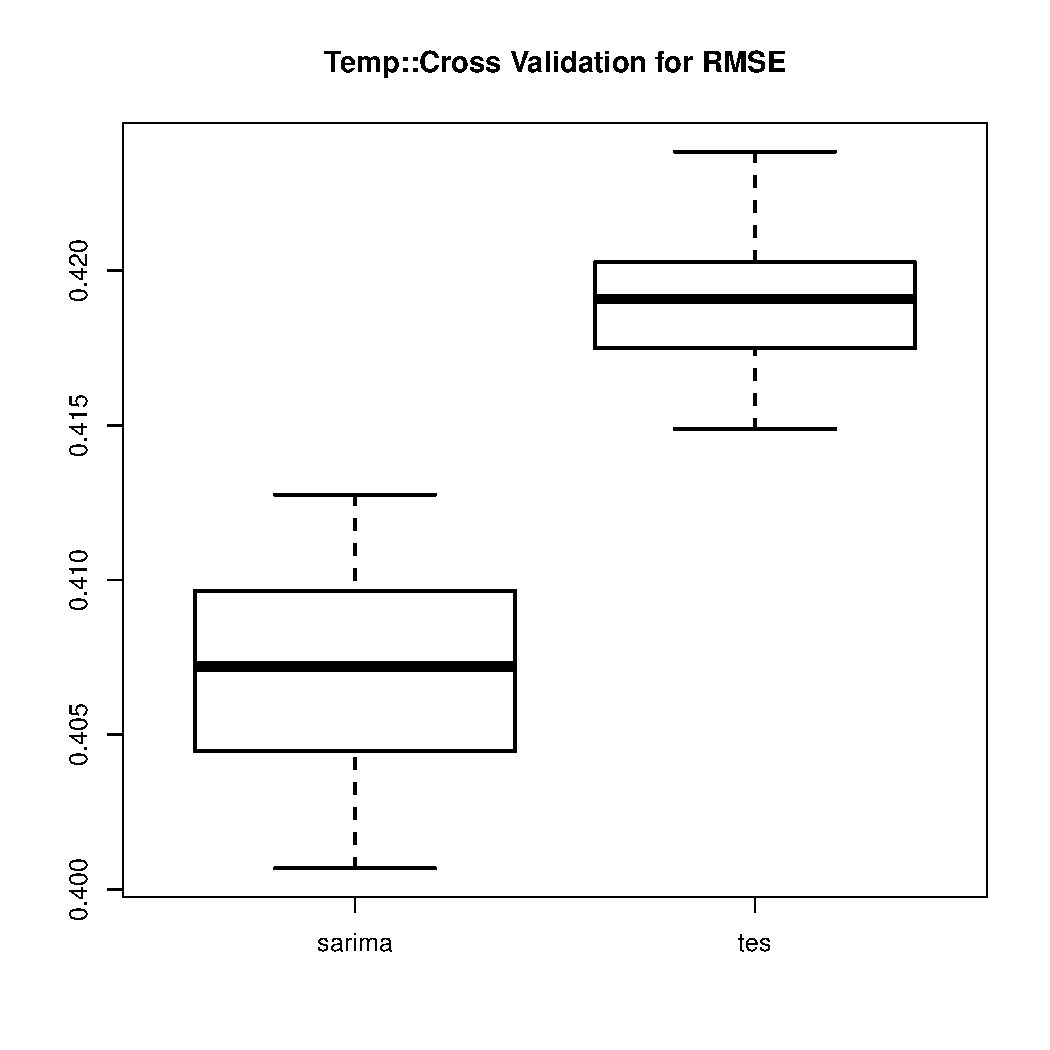
\includegraphics[width=\maxwidth]{figure/unnamed-chunk-30-1} 

\end{knitrout}
From boxplot, SARIMA(2,1,1)(0,1,1)[12] gives a better prediction, due to the lower RMSE.
\bigskip
6. Forecast the number of birth during the two weeks by using SARIMA(2,1,1)(0,1,1)[12] model.
\begin{knitrout}
\definecolor{shadecolor}{rgb}{0.969, 0.969, 0.969}\color{fgcolor}\begin{kframe}
\begin{alltt}
\hlstd{temp_forecast} \hlkwb{<-} \hlkwd{forecast}\hlstd{(temp_fit,} \hlkwc{h} \hlstd{=} \hlnum{2}\hlopt{*}\hlnum{12}\hlstd{)}
\hlstd{temp_forecast}
\end{alltt}
\begin{verbatim}
##          Point Forecast    Lo 80    Hi 80    Lo 95    Hi 95
## Jul 2016       28.37633 27.83817 28.91450 27.55328 29.19939
## Aug 2016       28.21659 27.63264 28.80053 27.32352 29.10966
## Sep 2016       28.13355 27.51165 28.75546 27.18243 29.08468
## Oct 2016       28.09030 27.45209 28.72852 27.11424 29.06637
## Nov 2016       27.47766 26.82966 28.12567 26.48662 28.46870
## Dec 2016       26.96136 26.30782 27.61489 25.96186 27.96085
## Jan 2017       27.04456 26.38762 27.70149 26.03986 28.04926
## Feb 2017       27.63363 26.97449 28.29277 26.62556 28.64170
## Mar 2017       28.07603 27.41536 28.73670 27.06562 29.08644
## Apr 2017       28.50624 27.84445 29.16803 27.49412 29.51836
## May 2017       28.84737 28.18470 29.51003 27.83391 29.86082
## Jun 2017       28.85382 28.19044 29.51720 27.83926 29.86837
## Jul 2017       28.43358 27.76872 29.09844 27.41676 29.45040
## Aug 2017       28.32352 27.65779 28.98925 27.30538 29.34166
## Sep 2017       28.19824 27.53172 28.86476 27.17888 29.21759
## Oct 2017       28.14836 27.48117 28.81556 27.12798 29.16875
## Nov 2017       27.52417 26.85636 28.19198 26.50284 28.54550
## Dec 2017       27.00181 26.33343 27.67020 25.97961 28.02402
## Jan 2018       27.08014 26.41124 27.74904 26.05715 28.10313
## Feb 2018       27.66597 26.99660 28.33534 26.64226 28.68968
## Mar 2018       28.10604 27.43622 28.77586 27.08164 29.13044
## Apr 2018       28.53463 27.86437 29.20489 27.50955 29.55971
## May 2018       28.87461 28.20390 29.54531 27.84885 29.90036
## Jun 2018       28.88025 28.20911 29.55139 27.85383 29.90667
\end{verbatim}
\begin{alltt}
\hlkwd{plot}\hlstd{(temp_forecast,} \hlkwc{main} \hlstd{=} \hlstr{"Temperature Forecasts from SARIMA(2,1,1)(0,1,1)[12]"}\hlstd{,}\hlkwc{lwd} \hlstd{=} \hlnum{2}\hlstd{)}
\end{alltt}
\end{kframe}
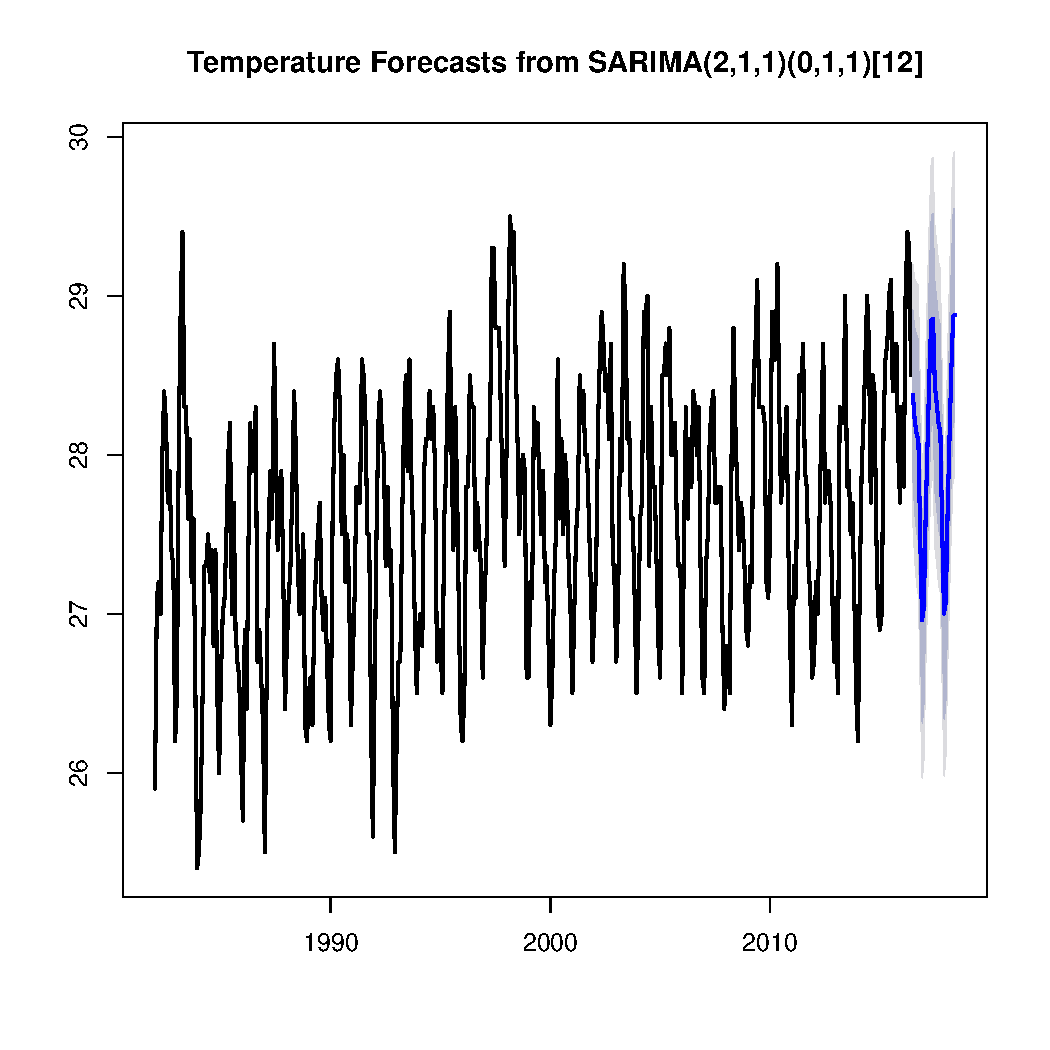
\includegraphics[width=\maxwidth]{figure/unnamed-chunk-31-1} 

\end{knitrout}


\section{ Exercise 5 (Monthly Car Sales in Quebuc?)}

1. Load the data and plot.
\begin{knitrout}
\definecolor{shadecolor}{rgb}{0.969, 0.969, 0.969}\color{fgcolor}\begin{kframe}
\begin{alltt}
\hlstd{carSale_data} \hlkwb{<-} \hlkwd{read.csv}\hlstd{(}\hlstr{"E:/ST3233/Assignment2/Datasets/monthly-car-sales-in-quebec-1960.csv"}\hlstd{,}
                         \hlkwc{header}\hlstd{=} \hlnum{TRUE}\hlstd{,}\hlkwc{sep}\hlstd{=}\hlstr{","}\hlstd{)}
\hlstd{carSale} \hlkwb{<-} \hlkwd{ts}\hlstd{(carSale_data}\hlopt{$}\hlstd{Monthly.car.sales.in.Quebec.1960.1968[}\hlnum{1}\hlopt{:}\hlnum{108}\hlstd{],}
              \hlkwc{frequency} \hlstd{=} \hlnum{12}\hlstd{,}\hlkwc{start}\hlstd{=}\hlkwd{c}\hlstd{(}\hlnum{1960}\hlstd{,}\hlnum{1}\hlstd{))}
\hlkwd{par}\hlstd{(}\hlkwc{mfrow}\hlstd{=}\hlkwd{c}\hlstd{(}\hlnum{1}\hlstd{,}\hlnum{1}\hlstd{))}
\hlkwd{plot}\hlstd{(carSale,}\hlkwc{lwd} \hlstd{=} \hlnum{2}\hlstd{,} \hlkwc{main} \hlstd{=} \hlstr{"monthly car sales"}\hlstd{)}
\end{alltt}
\end{kframe}
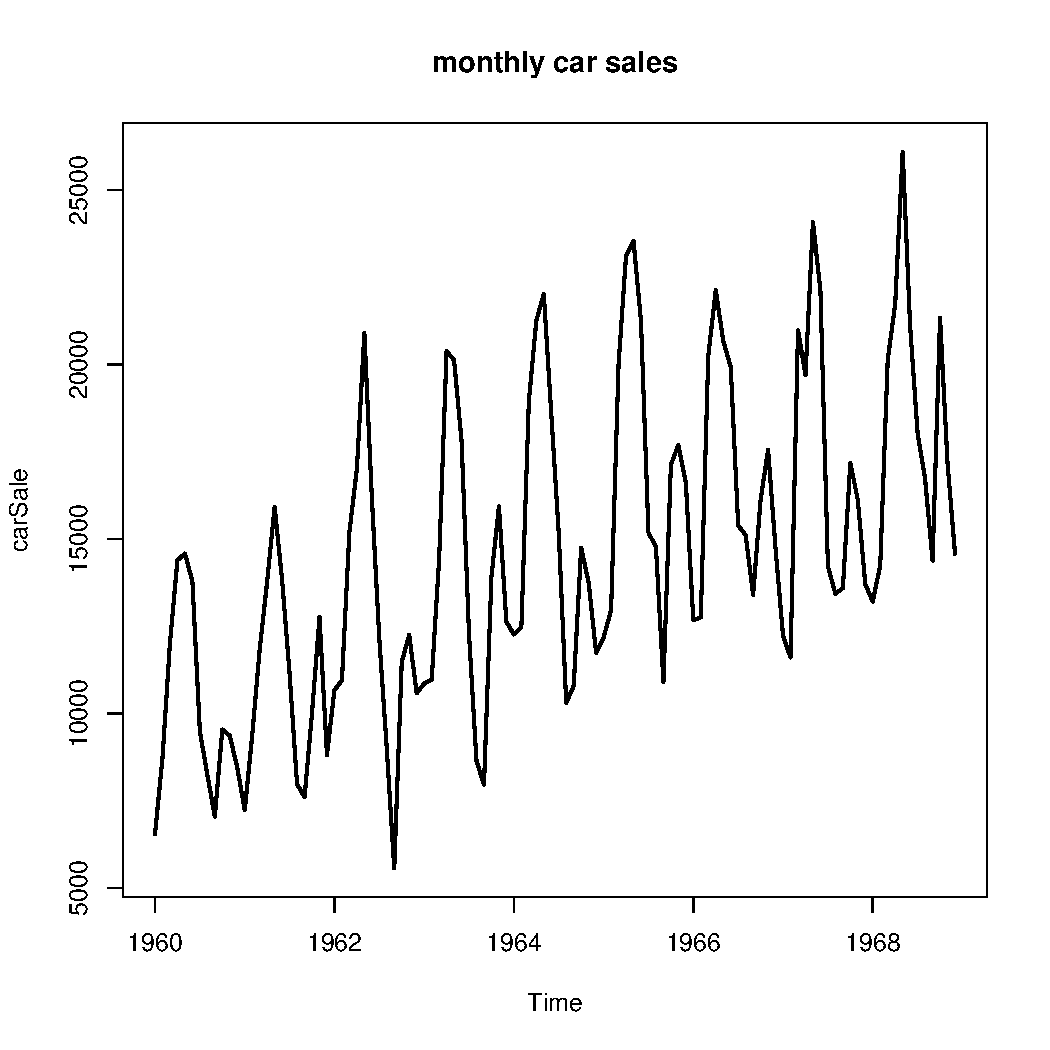
\includegraphics[width=\maxwidth]{figure/unnamed-chunk-32-1} 
\begin{kframe}\begin{alltt}
\hlkwd{acf}\hlstd{(carSale,}\hlkwc{lwd} \hlstd{=} \hlnum{2} \hlstd{,} \hlkwc{main} \hlstd{=} \hlstr{"ACF::carSale"}\hlstd{)}
\end{alltt}
\end{kframe}
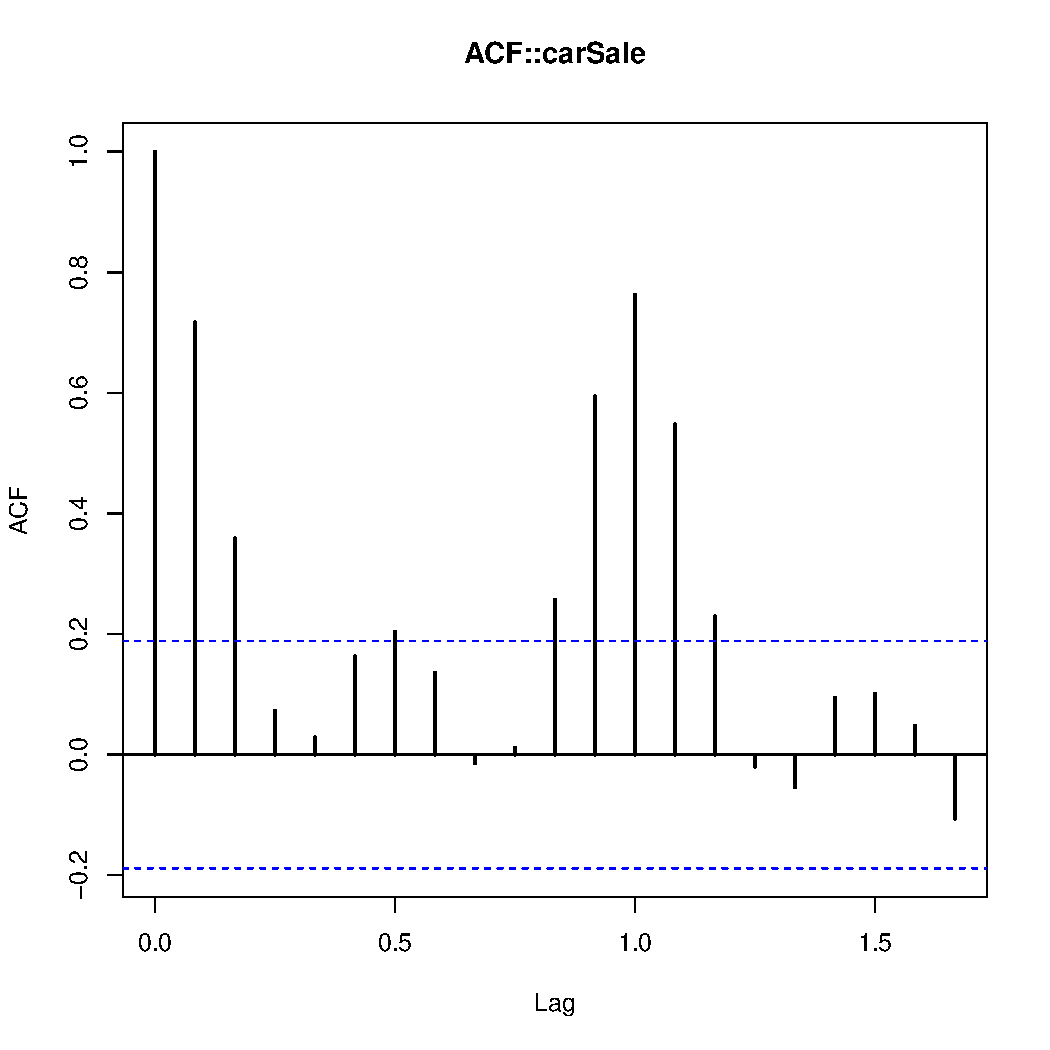
\includegraphics[width=\maxwidth]{figure/unnamed-chunk-32-2} 
\begin{kframe}\begin{alltt}
\hlcom{#The time series is not stationary and has periodicity and trend.}

\hlstd{carSale_decmp} \hlkwb{<-}\hlkwd{stl}\hlstd{(carSale,} \hlkwc{s.window} \hlstd{=} \hlstr{"periodic"}\hlstd{,} \hlkwc{robust} \hlstd{= T)}
\hlkwd{plot}\hlstd{(carSale_decmp)}
\end{alltt}
\end{kframe}
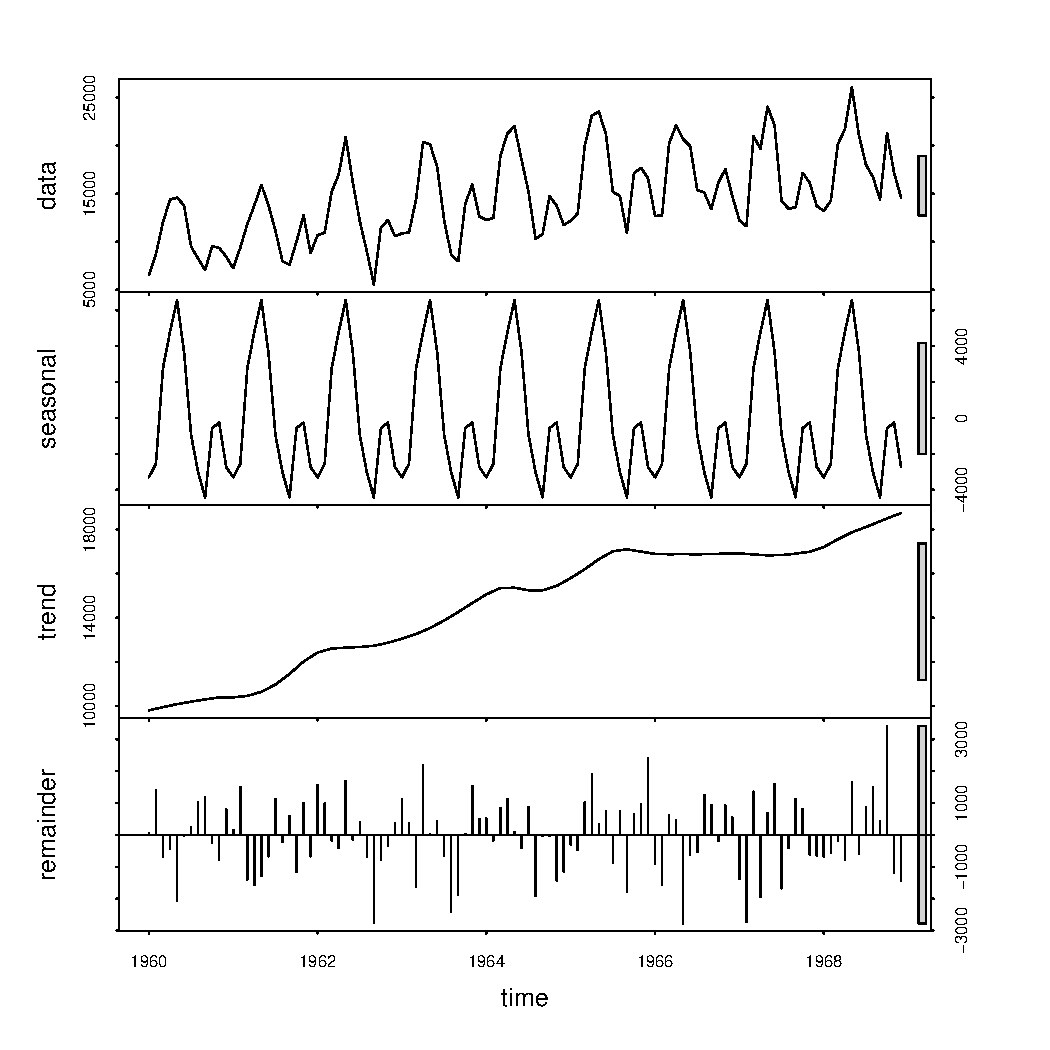
\includegraphics[width=\maxwidth]{figure/unnamed-chunk-32-3} 
\begin{kframe}\begin{alltt}
\hlkwd{seasonplot}\hlstd{(carSale}\hlopt{-}\hlstd{carSale_decmp}\hlopt{$}\hlstd{time.series[,}\hlstr{"trend"}\hlstd{],}\hlkwc{s} \hlstd{=} \hlnum{12}\hlstd{,} \hlkwc{col} \hlstd{=} \hlnum{1}\hlopt{:}\hlnum{12}\hlstd{,} \hlkwc{type} \hlstd{=} \hlstr{"l"}\hlstd{)}
\end{alltt}
\end{kframe}
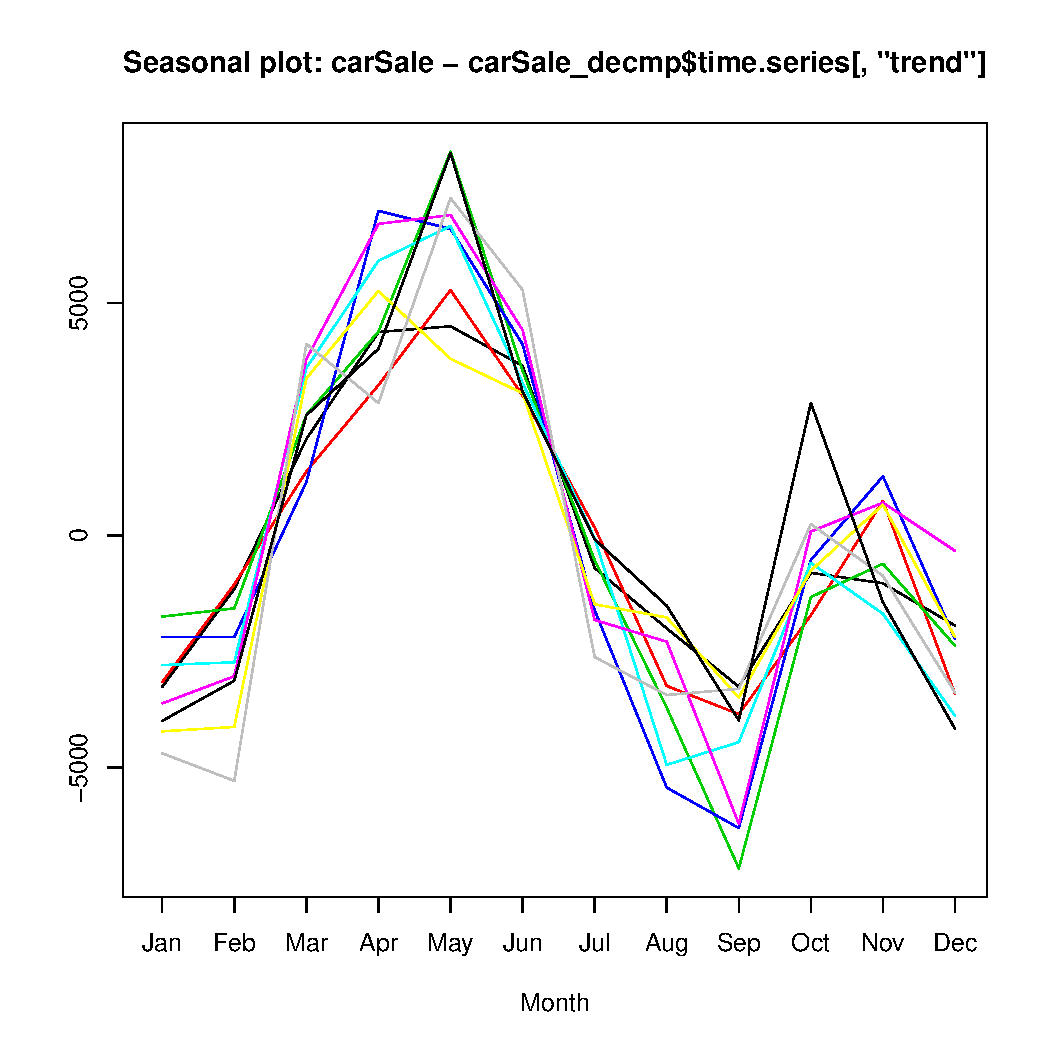
\includegraphics[width=\maxwidth]{figure/unnamed-chunk-32-4} 

\end{knitrout}
There is seasonal component and trend, thus, use SARIMA model
\bigskip
2.First fit the SARIMA model.
\begin{knitrout}
\definecolor{shadecolor}{rgb}{0.969, 0.969, 0.969}\color{fgcolor}\begin{kframe}
\begin{alltt}
\hlstd{carSale_d12} \hlkwb{=} \hlkwd{diff}\hlstd{(carSale,} \hlkwc{lag} \hlstd{=} \hlnum{12}\hlstd{)}
\hlkwd{plot}\hlstd{(carSale_d12,}\hlkwc{lwd} \hlstd{=} \hlnum{2}\hlstd{,} \hlkwc{main} \hlstd{=} \hlstr{"diff(carSale, lag = 12)"}\hlstd{)}
\end{alltt}
\end{kframe}
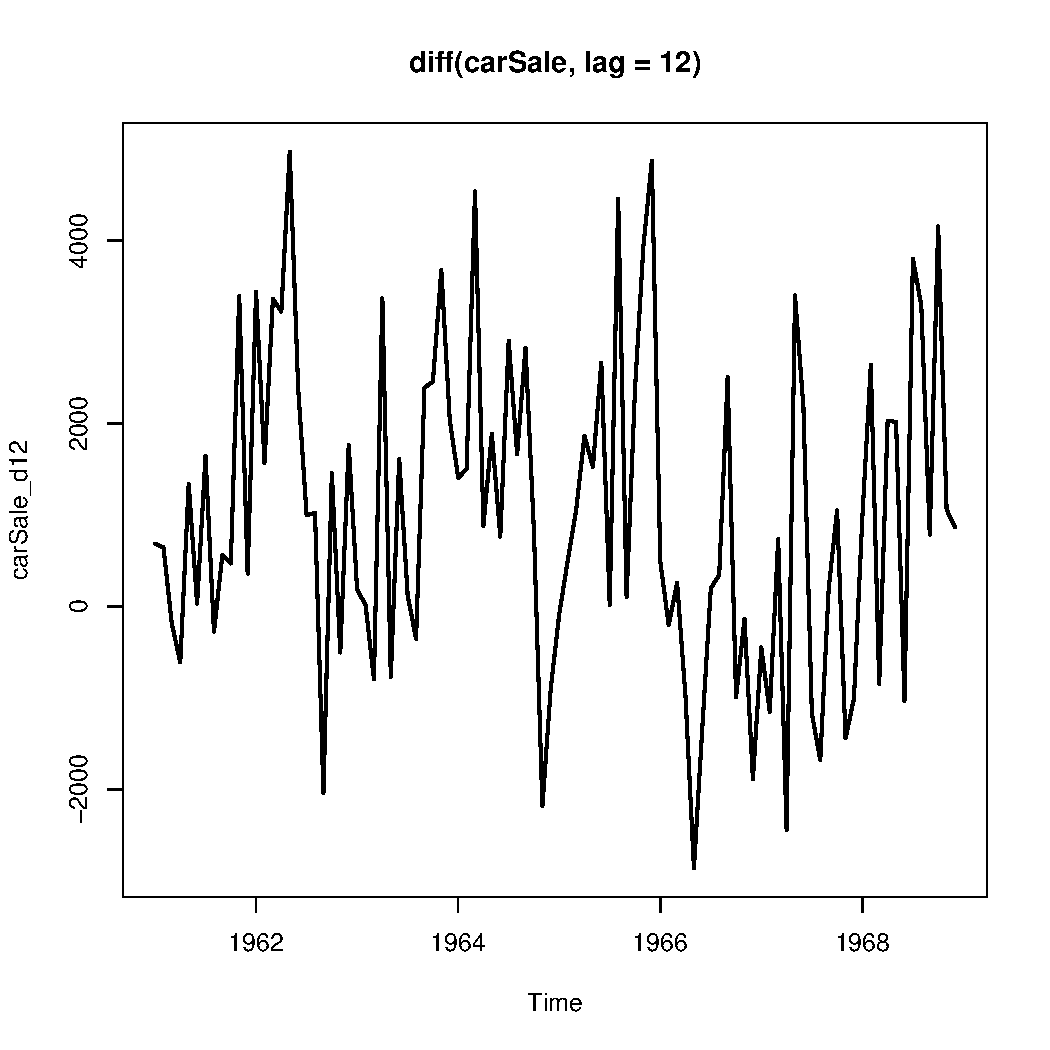
\includegraphics[width=\maxwidth]{figure/unnamed-chunk-33-1} 
\begin{kframe}\begin{alltt}
\hlkwd{acf}\hlstd{(carSale_d12,}\hlkwc{lwd} \hlstd{=} \hlnum{2}\hlstd{,} \hlkwc{main} \hlstd{=}\hlstr{"ACF::diff(carSale, lag = 12)"}\hlstd{)}
\end{alltt}
\end{kframe}
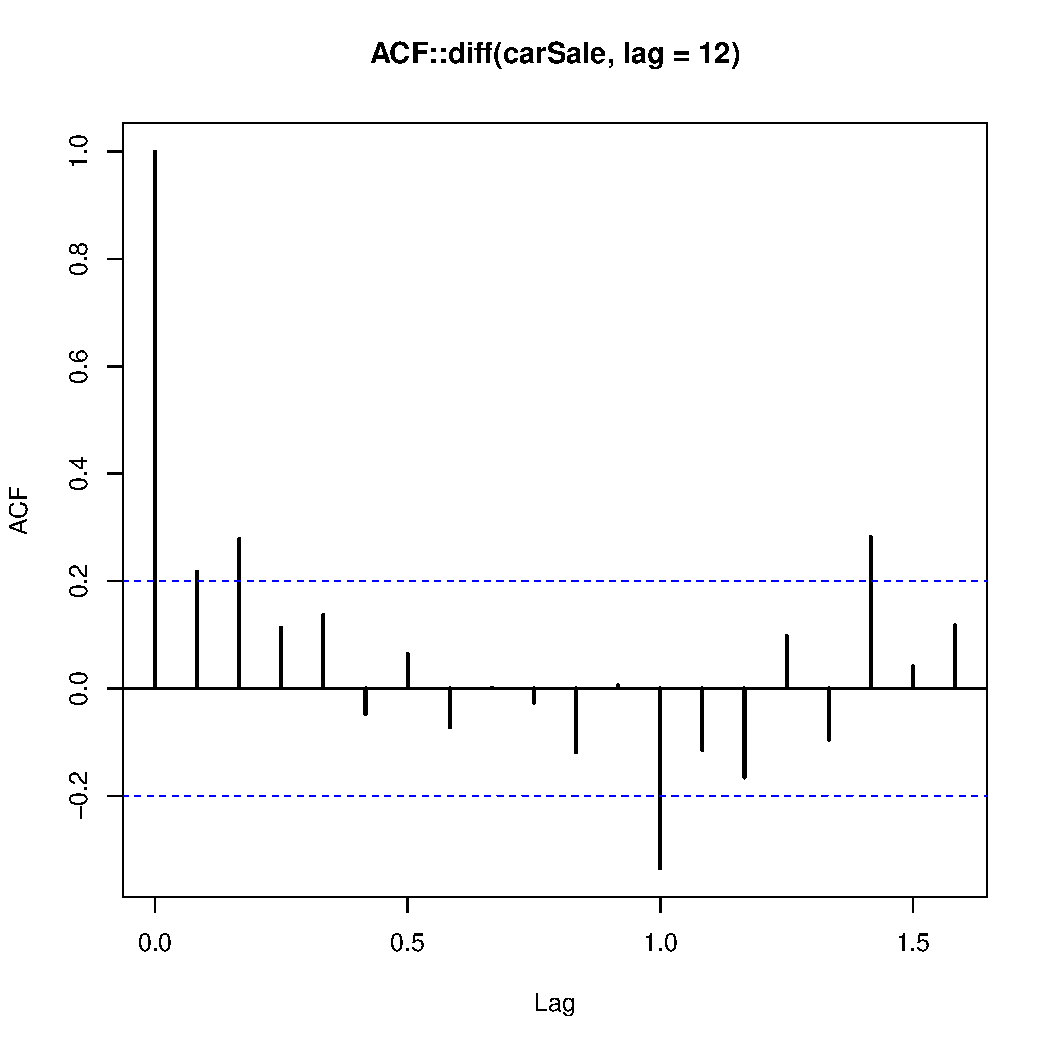
\includegraphics[width=\maxwidth]{figure/unnamed-chunk-33-2} 
\begin{kframe}\begin{alltt}
\hlcom{#carSale_d12 is not stationary, consider diff(carSale_d12)}

\hlstd{carSale_d12_d1} \hlkwb{=} \hlkwd{diff}\hlstd{(carSale_d12,} \hlkwc{lag} \hlstd{=} \hlnum{1}\hlstd{)}
\hlkwd{plot}\hlstd{(carSale_d12_d1,}\hlkwc{lwd} \hlstd{=} \hlnum{2}\hlstd{,} \hlkwc{main} \hlstd{=} \hlstr{"diff(diff(carSale, lag = 12))"}\hlstd{)}
\end{alltt}
\end{kframe}
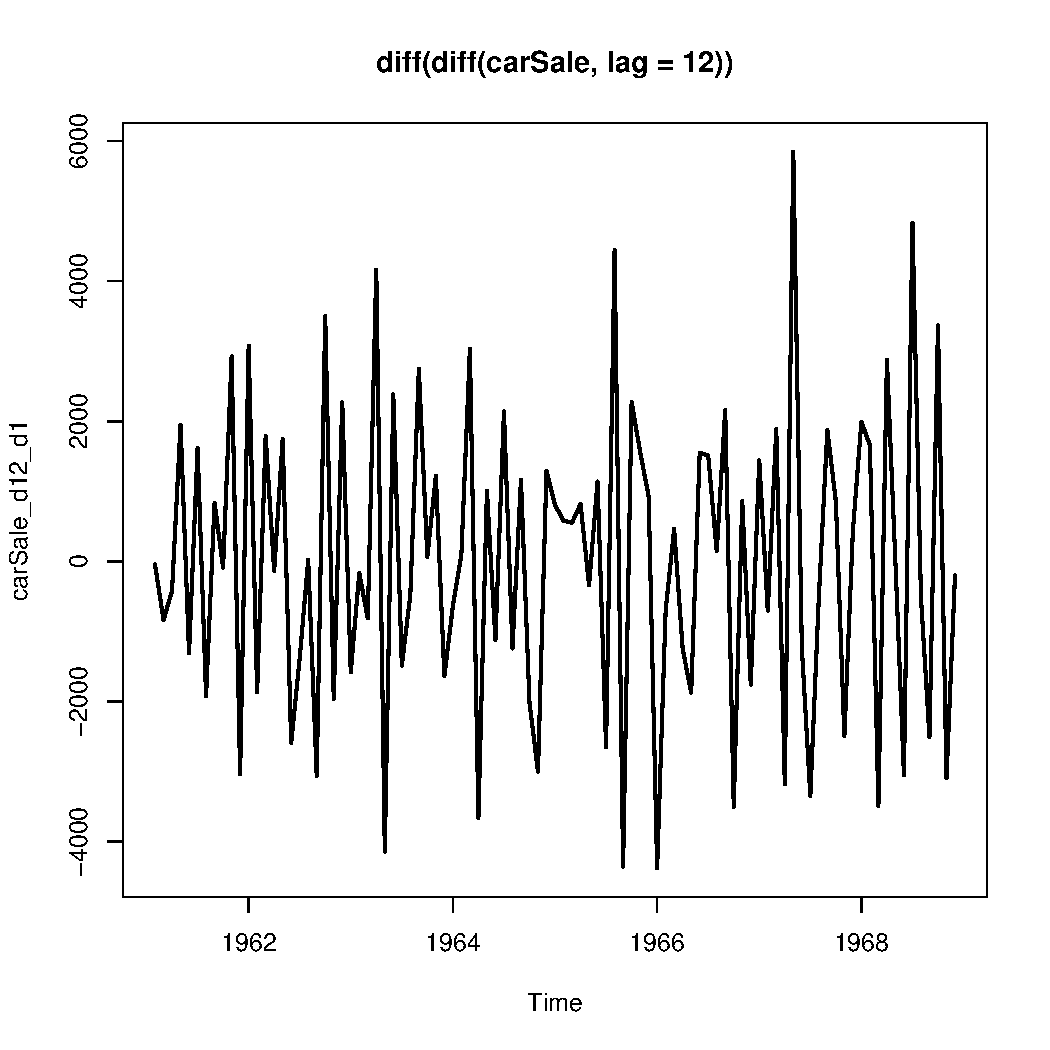
\includegraphics[width=\maxwidth]{figure/unnamed-chunk-33-3} 
\begin{kframe}\begin{alltt}
\hlkwd{par}\hlstd{(}\hlkwc{mfrow}\hlstd{=}\hlkwd{c}\hlstd{(}\hlnum{2}\hlstd{,}\hlnum{1}\hlstd{))}
\hlkwd{acf}\hlstd{(carSale_d12_d1,}\hlkwc{lwd} \hlstd{=} \hlnum{2}\hlstd{,} \hlkwc{main} \hlstd{=} \hlstr{"ACF::diff(diff(carSale, lag = 12))"}\hlstd{)}
\hlkwd{pacf}\hlstd{(carSale_d12_d1,}\hlkwc{lwd} \hlstd{=} \hlnum{2}\hlstd{,} \hlkwc{main} \hlstd{=} \hlstr{"PACF::diff(diff(carSale, lag = 12))"}\hlstd{)}
\end{alltt}
\end{kframe}
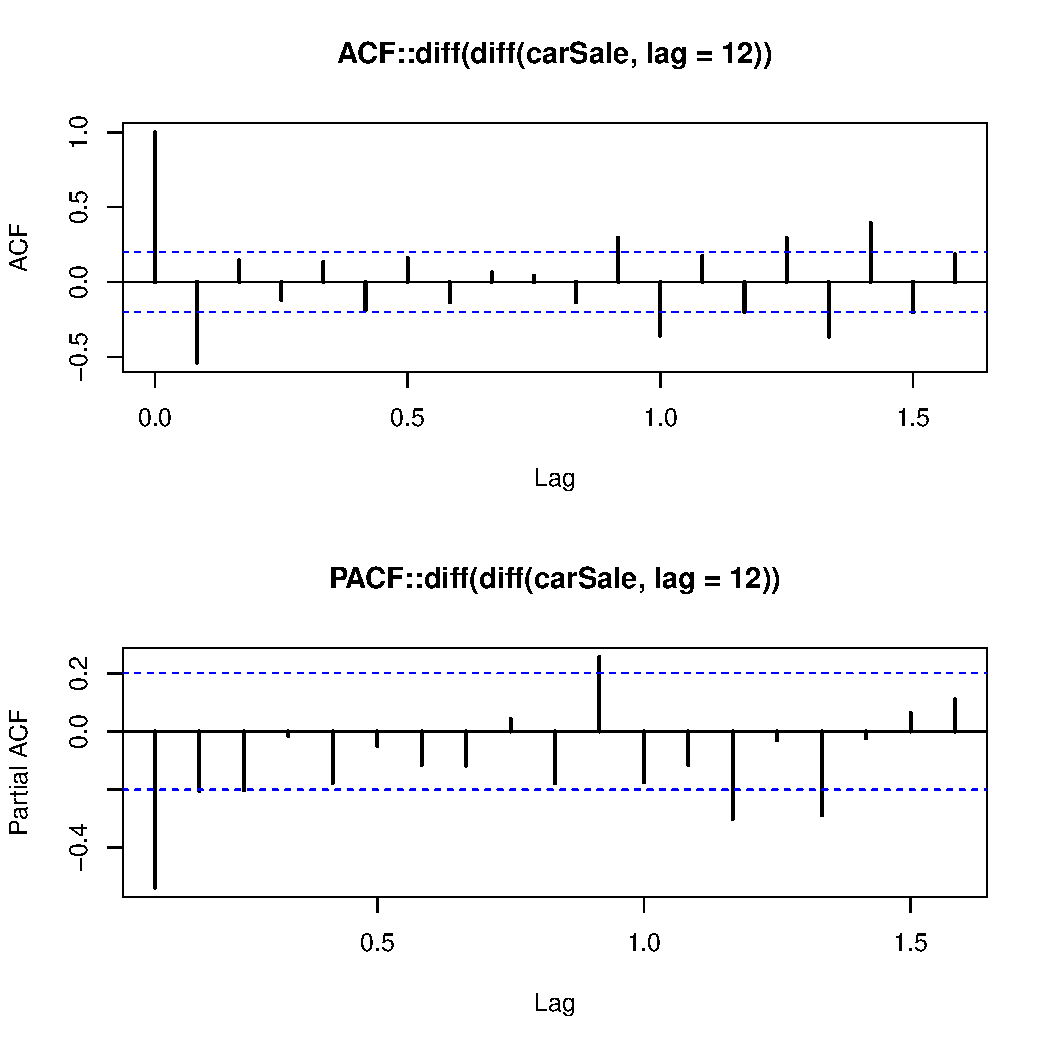
\includegraphics[width=\maxwidth]{figure/unnamed-chunk-33-4} 

\end{knitrout}
From acf plot ,q \leq 1, and from partial-acf plot, p \leq 2 with d = D = 1 and P \leq 1, Q \leq 1

\begin{knitrout}
\definecolor{shadecolor}{rgb}{0.969, 0.969, 0.969}\color{fgcolor}\begin{kframe}
\begin{alltt}
\hlstd{AIC_best} \hlkwb{<-} \hlnum{10}\hlopt{**}\hlnum{6}
\hlkwa{for} \hlstd{(p} \hlkwa{in} \hlnum{0}\hlopt{:}\hlnum{2}\hlstd{)\{}
  \hlkwa{for} \hlstd{(q} \hlkwa{in} \hlnum{0}\hlopt{:}\hlnum{1}\hlstd{)\{}
    \hlkwa{for} \hlstd{(P} \hlkwa{in} \hlnum{0}\hlopt{:}\hlnum{1}\hlstd{)\{}
      \hlkwa{for} \hlstd{(Q} \hlkwa{in} \hlnum{0}\hlopt{:}\hlnum{1}\hlstd{)\{}
        \hlstd{fit_sarima} \hlkwb{<-} \hlkwd{Arima}\hlstd{(carSale,} \hlkwc{order} \hlstd{=} \hlkwd{c}\hlstd{(p,}\hlnum{1}\hlstd{,q),}\hlkwc{seasonal} \hlstd{=} \hlkwd{c}\hlstd{(P,}\hlnum{1}\hlstd{,Q))}
        \hlkwa{if} \hlstd{(fit_sarima}\hlopt{$}\hlstd{aic} \hlopt{<} \hlstd{AIC_best)\{}
          \hlstd{AIC_best} \hlkwb{<-} \hlstd{fit_sarima}\hlopt{$}\hlstd{aic}
          \hlkwd{cat}\hlstd{(}\hlstr{"p = "}\hlstd{,p,}\hlstr{", q = "}\hlstd{,q,}\hlstr{",P = "}\hlstd{,P,}\hlstr{",Q = "}\hlstd{,Q,}\hlstr{"\textbackslash{}t AIC = "}\hlstd{,AIC_best,}\hlstr{"\textbackslash{}n"}\hlstd{)}
        \hlstd{\}}
      \hlstd{\}}
    \hlstd{\}}
  \hlstd{\}}
\hlstd{\}}
\end{alltt}
\begin{verbatim}
## p =  0 , q =  0 ,P =  0 ,Q =  0 	 AIC =  1734.779 
## p =  0 , q =  0 ,P =  0 ,Q =  1 	 AIC =  1712.686 
## p =  0 , q =  1 ,P =  0 ,Q =  0 	 AIC =  1694.382 
## p =  0 , q =  1 ,P =  0 ,Q =  1 	 AIC =  1676.588
\end{verbatim}
\end{kframe}
\end{knitrout}
The lowest AIC gives the best fitted model, which is SARIMA(0,1,1)(0,1,1)[12]

\begin{knitrout}
\definecolor{shadecolor}{rgb}{0.969, 0.969, 0.969}\color{fgcolor}\begin{kframe}
\begin{alltt}
\hlstd{carSale_fit} \hlkwb{<-} \hlkwd{Arima}\hlstd{(carSale,} \hlkwc{order} \hlstd{=} \hlkwd{c}\hlstd{(}\hlnum{0}\hlstd{,}\hlnum{1}\hlstd{,}\hlnum{1}\hlstd{),} \hlkwc{seasonal} \hlstd{=} \hlkwd{c}\hlstd{(}\hlnum{0}\hlstd{,}\hlnum{1}\hlstd{,}\hlnum{1}\hlstd{))}
\end{alltt}
\end{kframe}
\end{knitrout}

3. Then consider the residuals of the SARIMA model.
\begin{knitrout}
\definecolor{shadecolor}{rgb}{0.969, 0.969, 0.969}\color{fgcolor}\begin{kframe}
\begin{alltt}
\hlkwd{par}\hlstd{(}\hlkwc{mfrow}\hlstd{=}\hlkwd{c}\hlstd{(}\hlnum{1}\hlstd{,}\hlnum{1}\hlstd{))}
\hlkwd{plot}\hlstd{(}\hlkwd{resid}\hlstd{(carSale_fit),}\hlkwc{lwd}\hlstd{=}\hlnum{2}\hlstd{,} \hlkwc{main}\hlstd{=}\hlstr{"resid(SARIMA(0,1,1)(0,1,1)[12])"}\hlstd{)}
\end{alltt}
\end{kframe}
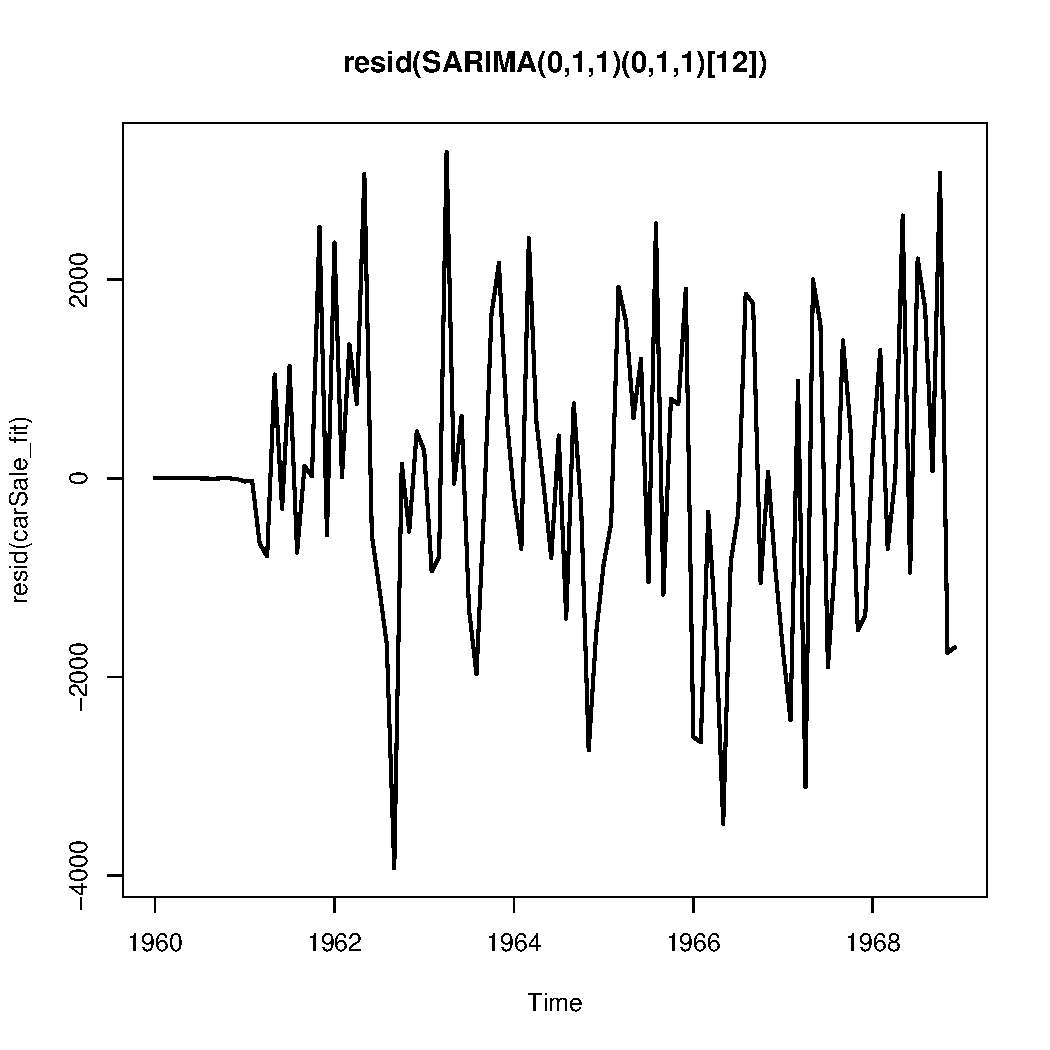
\includegraphics[width=\maxwidth]{figure/unnamed-chunk-36-1} 
\begin{kframe}\begin{alltt}
\hlkwd{par}\hlstd{(}\hlkwc{mfrow}\hlstd{=}\hlkwd{c}\hlstd{(}\hlnum{2}\hlstd{,}\hlnum{1}\hlstd{))}
\hlkwd{acf}\hlstd{(}\hlkwd{resid}\hlstd{(carSale_fit),}\hlkwc{lwd}\hlstd{=}\hlnum{2}\hlstd{,} \hlkwc{main}\hlstd{=}\hlstr{"ACF::resid(SARIMA(0,1,1)(0,1,1)[12])"}\hlstd{,}\hlkwc{lag.max} \hlstd{=} \hlnum{11}\hlstd{)}
\hlkwd{pacf}\hlstd{(}\hlkwd{resid}\hlstd{(carSale_fit),}\hlkwc{lwd}\hlstd{=}\hlnum{2}\hlstd{,} \hlkwc{main}\hlstd{=}\hlstr{"PACF::resid(SARIMA(0,1,1)(0,1,1)[12])"}\hlstd{,}\hlkwc{lag.max} \hlstd{=} \hlnum{11}\hlstd{)}
\end{alltt}
\end{kframe}
\includegraphics[width=\maxwidth]{figure/unnamed-chunk-36-2} 
\begin{kframe}\begin{alltt}
\hlcom{#The residual is stationary.}
\hlkwd{par}\hlstd{(}\hlkwc{mfrow}\hlstd{=}\hlkwd{c}\hlstd{(}\hlnum{1}\hlstd{,}\hlnum{1}\hlstd{))}
\hlkwd{qqnorm}\hlstd{(}\hlkwd{resid}\hlstd{(carSale_fit),}\hlkwc{lwd}\hlstd{=}\hlnum{2}\hlstd{,} \hlkwc{main}\hlstd{=}\hlstr{"QQplot::resid(SARIMA(0,1,1)(0,1,1)[12])"}\hlstd{)}
\hlkwd{qqline}\hlstd{(}\hlkwd{resid}\hlstd{(carSale_fit),} \hlkwc{lwd}\hlstd{=}\hlnum{2}\hlstd{,} \hlkwc{col}\hlstd{=}\hlstr{"red"}\hlstd{)}
\end{alltt}
\end{kframe}
\includegraphics[width=\maxwidth]{figure/unnamed-chunk-36-3} 
\begin{kframe}\begin{alltt}
\hlkwd{shapiro.test}\hlstd{(}\hlkwd{resid}\hlstd{(carSale_fit))}
\end{alltt}
\begin{verbatim}
## 
## 	Shapiro-Wilk normality test
## 
## data:  resid(carSale_fit)
## W = 0.98601, p-value = 0.3211
\end{verbatim}
\end{kframe}
\end{knitrout}
From the qq-plot and Shapiro test(p-value = 0.3211>0.05), the residual can be regard as a gaussian distribution.
So, SARIMA(0,1,1)(0,1,1)[12] is a good model.
\bigskip
4. Another method is using Triple exponential smoothing

\begin{knitrout}
\definecolor{shadecolor}{rgb}{0.969, 0.969, 0.969}\color{fgcolor}\begin{kframe}
\begin{alltt}
\hlstd{TES_fit} \hlkwb{<-} \hlkwd{hw}\hlstd{(carSale,} \hlkwc{initial} \hlstd{=} \hlstr{"optimal"}\hlstd{,} \hlkwc{seasonal} \hlstd{=} \hlstr{"additive"}\hlstd{,} \hlkwc{h} \hlstd{=} \hlnum{2}\hlopt{*}\hlnum{12}\hlstd{)}
\hlstd{TES_fit}
\end{alltt}
\begin{verbatim}
##          Point Forecast    Lo 80    Hi 80    Lo 95    Hi 95
## Jan 1969       15404.76 13672.55 17136.96 12755.58 18053.94
## Feb 1969       16126.19 14365.75 17886.62 13433.83 18818.54
## Mar 1969       21926.35 20137.72 23714.98 19190.87 24661.83
## Apr 1969       24093.96 22277.16 25910.76 21315.40 26872.52
## May 1969       25871.41 24026.46 27716.35 23049.81 28693.00
## Jun 1969       23075.58 21202.51 24948.64 20210.97 25940.19
## Jul 1969       18388.86 16487.69 20290.03 15481.28 21296.45
## Aug 1969       16231.14 14301.88 18160.40 13280.60 19181.69
## Sep 1969       14931.16 12973.82 16888.50 11937.67 17924.65
## Oct 1969       19290.16 17304.74 21275.57 16253.73 22326.59
## Nov 1969       19768.70 17755.22 21782.19 16689.35 22848.06
## Dec 1969       17494.59 15453.01 19536.17 14372.26 20616.91
## Jan 1970       16572.93 14503.28 18642.58 13407.67 19738.18
## Feb 1970       17294.36 15196.64 19392.08 14086.17 20502.54
## Mar 1970       23094.52 20968.72 25220.32 19843.39 26345.65
## Apr 1970       25262.13 23108.24 27416.02 21968.04 28556.22
## May 1970       27039.58 24857.59 29221.56 23702.52 30376.64
## Jun 1970       24243.75 22033.65 26453.85 20863.70 27623.80
## Jul 1970       19557.03 17318.81 21795.26 16133.97 22980.10
## Aug 1970       17399.31 15132.95 19665.68 13933.21 20865.42
## Sep 1970       16099.33 13804.80 18393.86 12590.15 19608.51
## Oct 1970       20458.33 18135.62 22781.04 16906.05 24010.61
## Nov 1970       20936.87 18585.96 23287.79 17341.47 24532.28
## Dec 1970       18662.76 16283.59 21041.92 15024.14 22301.37
\end{verbatim}
\begin{alltt}
\hlkwd{plot}\hlstd{(TES_fit,}\hlkwc{main} \hlstd{=} \hlstr{"Car Sales Forecasts from Triple Exponential Smoothing"}\hlstd{,} \hlkwc{lwd} \hlstd{=} \hlnum{2}\hlstd{)}
\end{alltt}
\end{kframe}
\includegraphics[width=\maxwidth]{figure/unnamed-chunk-37-1} 

\end{knitrout}

5. Use cross-validation to compare these two models
\begin{knitrout}
\definecolor{shadecolor}{rgb}{0.969, 0.969, 0.969}\color{fgcolor}\begin{kframe}
\begin{alltt}
\hlstd{CV} \hlkwb{<-}  \hlkwa{function}\hlstd{(}\hlkwc{time_series}\hlstd{,} \hlkwc{start}\hlstd{,} \hlkwc{forecast_length}\hlstd{,}\hlkwc{ts_model}\hlstd{)\{}
  \hlstd{ts_length} \hlkwb{<-}  \hlkwd{length}\hlstd{(time_series)}
  \hlstd{accuracy_list} \hlkwb{=} \hlkwd{c}\hlstd{()}
  \hlkwa{for}\hlstd{(k} \hlkwa{in} \hlstd{start}\hlopt{:}\hlstd{(ts_length} \hlopt{-} \hlstd{forecast_length))\{}
    \hlstd{fitted_model} \hlkwb{<-} \hlkwd{ts_model}\hlstd{(}\hlkwd{ts}\hlstd{(time_series[}\hlnum{0}\hlopt{:}\hlstd{k],}\hlkwc{frequency} \hlstd{=} \hlnum{12}\hlstd{))}
    \hlstd{RMSE} \hlkwb{<-}  \hlkwd{accuracy}\hlstd{(}\hlkwd{forecast}\hlstd{(fitted_model,} \hlkwc{h} \hlstd{= forecast_length))[}\hlnum{2}\hlstd{]}
    \hlstd{accuracy_list} \hlkwb{=} \hlkwd{c}\hlstd{(accuracy_list, RMSE)}
  \hlstd{\}}
  \hlkwd{return}\hlstd{(accuracy_list)}
\hlstd{\}}

\hlstd{model_SARIMA} \hlkwb{<-} \hlkwa{function}\hlstd{(}\hlkwc{ts}\hlstd{)}
  \hlkwd{return}\hlstd{(}\hlkwd{Arima}\hlstd{(ts,} \hlkwc{order} \hlstd{=} \hlkwd{c}\hlstd{(}\hlnum{0}\hlstd{,}\hlnum{1}\hlstd{,}\hlnum{1}\hlstd{),} \hlkwc{seasonal} \hlstd{=} \hlkwd{c}\hlstd{(}\hlnum{0}\hlstd{,}\hlnum{1}\hlstd{,}\hlnum{1}\hlstd{)))}
\hlstd{model_TES} \hlkwb{<-} \hlkwa{function}\hlstd{(}\hlkwc{ts}\hlstd{)}
  \hlkwd{return}\hlstd{(}\hlkwd{hw}\hlstd{(ts,}\hlkwc{initial} \hlstd{=} \hlstr{"optimal"}\hlstd{,} \hlkwc{seasonal} \hlstd{=} \hlstr{"additive"}\hlstd{))}

\hlstd{start} \hlkwb{<-} \hlnum{60}
\hlstd{forecast_length} \hlkwb{<-} \hlnum{2}\hlopt{*}\hlnum{12}
\hlstd{CV_carSale} \hlkwb{<-} \hlkwd{data.frame}\hlstd{(}
  \hlkwc{sarima} \hlstd{=} \hlkwd{CV}\hlstd{(carSale, start, forecast_length, model_SARIMA),}
  \hlkwc{tes} \hlstd{=} \hlkwd{CV}\hlstd{(carSale, start, forecast_length, model_TES)}
\hlstd{)}

\hlkwd{boxplot}\hlstd{(CV_carSale,}\hlkwc{main} \hlstd{=} \hlstr{"Car Sales::Cross Validation for RMSE"}\hlstd{,} \hlkwc{lwd}\hlstd{=}\hlnum{2}\hlstd{)}
\end{alltt}
\end{kframe}
\includegraphics[width=\maxwidth]{figure/unnamed-chunk-38-1} 

\end{knitrout}
From boxplot, TES gives a better prediction due to the lower RMSE.
\bigskip
6. Forecast the number of birth during the two weeks by using triple exponential smoothing.
\begin{knitrout}
\definecolor{shadecolor}{rgb}{0.969, 0.969, 0.969}\color{fgcolor}\begin{kframe}
\begin{alltt}
\hlstd{TES_fit} \hlkwb{<-} \hlkwd{hw}\hlstd{(carSale,} \hlkwc{initial} \hlstd{=} \hlstr{"optimal"}\hlstd{,} \hlkwc{seasonal} \hlstd{=} \hlstr{"additive"}\hlstd{,} \hlkwc{h} \hlstd{=} \hlnum{2}\hlopt{*}\hlnum{12}\hlstd{)}
\hlstd{TES_fit}
\end{alltt}
\begin{verbatim}
##          Point Forecast    Lo 80    Hi 80    Lo 95    Hi 95
## Jan 1969       15404.76 13672.55 17136.96 12755.58 18053.94
## Feb 1969       16126.19 14365.75 17886.62 13433.83 18818.54
## Mar 1969       21926.35 20137.72 23714.98 19190.87 24661.83
## Apr 1969       24093.96 22277.16 25910.76 21315.40 26872.52
## May 1969       25871.41 24026.46 27716.35 23049.81 28693.00
## Jun 1969       23075.58 21202.51 24948.64 20210.97 25940.19
## Jul 1969       18388.86 16487.69 20290.03 15481.28 21296.45
## Aug 1969       16231.14 14301.88 18160.40 13280.60 19181.69
## Sep 1969       14931.16 12973.82 16888.50 11937.67 17924.65
## Oct 1969       19290.16 17304.74 21275.57 16253.73 22326.59
## Nov 1969       19768.70 17755.22 21782.19 16689.35 22848.06
## Dec 1969       17494.59 15453.01 19536.17 14372.26 20616.91
## Jan 1970       16572.93 14503.28 18642.58 13407.67 19738.18
## Feb 1970       17294.36 15196.64 19392.08 14086.17 20502.54
## Mar 1970       23094.52 20968.72 25220.32 19843.39 26345.65
## Apr 1970       25262.13 23108.24 27416.02 21968.04 28556.22
## May 1970       27039.58 24857.59 29221.56 23702.52 30376.64
## Jun 1970       24243.75 22033.65 26453.85 20863.70 27623.80
## Jul 1970       19557.03 17318.81 21795.26 16133.97 22980.10
## Aug 1970       17399.31 15132.95 19665.68 13933.21 20865.42
## Sep 1970       16099.33 13804.80 18393.86 12590.15 19608.51
## Oct 1970       20458.33 18135.62 22781.04 16906.05 24010.61
## Nov 1970       20936.87 18585.96 23287.79 17341.47 24532.28
## Dec 1970       18662.76 16283.59 21041.92 15024.14 22301.37
\end{verbatim}
\begin{alltt}
\hlkwd{plot}\hlstd{(TES_fit,}\hlkwc{main} \hlstd{=} \hlstr{"Car Sales Forecasts from Triple Exponential Smoothing"}\hlstd{,} \hlkwc{lwd} \hlstd{=} \hlnum{2}\hlstd{)}
\end{alltt}
\end{kframe}
\includegraphics[width=\maxwidth]{figure/unnamed-chunk-39-1} 

\end{knitrout}

\end{document}
